\documentclass[11pt, spanish]{report}
\usepackage{geometry}
\usepackage{subfiles}
\usepackage{svg}
\geometry{margin=2cm}
\usepackage[utf8]{inputenc}
\usepackage[T1]{fontenc}
\usepackage[spanish]{babel}
\usepackage{amsmath, amsthm, amssymb}
\usepackage{mathrsfs}  
\usepackage{lscape}
\usepackage{multicol}
\usepackage[page,toc,titletoc,title]{appendix}
\usepackage{url}
\usepackage{listings}
\usepackage{tikz,pgfplots,pgf}
\pgfplotsset{compat=1.15}
\usepackage{enumitem}
\usepackage{epigraph}
\usepackage{tensor}
\usepackage{array}
\usepackage[breakable,skins]{tcolorbox}
\usepackage{physics}
\usepackage{endnotes}
\newcommand\ddfrac[2]{\frac{\displaystyle #1}{\displaystyle #2}}
\usepackage{lipsum}
\usepackage{caption}
\usepackage{subcaption}
\usepackage{algorithm}
\usepackage[noend]{algpseudocode}
\usepackage{systeme}
\usepackage{bbm}
\usepackage{yfonts}

%\usepackage{natbib}
\usepackage[export]{adjustbox}

\renewcommand{\baselinestretch}{1}
\newcommand{\bigslant}[2]{{\raisebox{.2em}{$#1$}\left/\raisebox{-.2em}{$#2$}\right.}}
\newcommand{\red}[1]{\textcolor{red}{#1}}

\DeclareMathOperator*{\argmax}{arg\,max}

%\usepackage{thmtools}
%\let\footnote=\endnote

\usepackage{chngcntr}
\counterwithin{figure}{section}
\numberwithin{equation}{section}

\usetikzlibrary{arrows}

\newcommand\Dist[1]{\phantom{\rule{#1}{4pt}}}

\usepackage{fancyhdr}
\setlength{\headheight}{15.2pt}
\pagestyle{fancy}
\renewcommand{\chaptermark}[1]{ \markboth{#1}{} }
\renewcommand{\sectionmark}[1]{ \markright{#1} }

\fancyhf{}
\fancyhead[LE,RO]{\thepage}
\fancyhead[RE]{\textit{ \nouppercase{\leftmark}} }
\fancyhead[LO]{\textit{ \nouppercase{\rightmark}} }

\fancypagestyle{plain}{ %
  \fancyhf{} % remove everything
  \renewcommand{\headrulewidth}{0pt} % remove lines as well
  \renewcommand{\footrulewidth}{0pt}
}

\usepackage[noautomatic]{imakeidx}
\usepackage{relsize}
\usepackage{graphicx}
\usepackage{todonotes}
\makeindex
\usepackage[nottoc]{tocbibind}

\newcommand{\myEq}[1]{\mathrel{\overset{\makebox[0pt]{\mbox{\normalfont\tiny\sffamily #1}}}{=}}} %Símbolo sobre el igual
\newcommand{\myEqUD}[2]{\mathrel{\overset{\makebox[0pt]{\mbox{\normalfont\tiny\sffamily #1}}}{\underset{\makebox[0pt]{\mbox{\normalfont\tiny\sffamily #2}}}{=}}}} %Símbolo sobre y bajo el igual

\newcommand{\Lagr}{\mathcal{L}}
%\renewcommand{\thesection}{\Roman{subsection}}

\newtheorem{defin}{Definición}[section]
\newtheorem{ejs}[defin]{Ejemplo}
\newtheorem{lema}[defin]{Lema}
\newtheorem{prop}[defin]{Proposición}
\newtheorem{teo}[defin]{Teorema}
\newtheorem{corol}[defin]{Corolario}
\newtheorem{nota}[defin]{Nota}
\newtheorem{hipot}[defin]{Hipótesis}
\newtheorem{postu}{Postulado}
\renewcommand\thepostu{\Roman{postu}}
\newtheorem{cuest}[defin]{Cuestión}
\newtheorem{obs}[defin]{Observación}
\newtheorem{ppio}[defin]{Principio}

\numberwithin{defin}{section}
%\numberwithin{ejs}{section}
%\numberwithin{prop}{section}
%\numberwithin{teo}{section}
%\numberwithin{corol}{section}

\usepackage{kantlipsum}
%\allowdisplaybreaks

\usepackage{hyperref}
\hypersetup{
    colorlinks,
    citecolor=black,
    filecolor=black,
    linkcolor=black,
    urlcolor=black
}

\renewcommand{\appendixtocname}{Ap\'endices}
\renewcommand{\appendixpagename}{Ap\'endices}

\makeatletter
\appto{\appendices}{\def\Hy@chapapp{Appendix}}
\makeatother
\usepackage{lettrine}


%\DeclareMathOperator{\atan}{atan}
\DeclareMathOperator{\Dom}{Dom}
\DeclareMathOperator{\mcd}{mcd}
\DeclareMathOperator{\bin}{bin}
\DeclareMathOperator{\interior}{int}
\DeclareMathOperator{\NP}{\mathbf{NP}}
\DeclareMathOperator{\PP}{\mathbf{P}}
\DeclareMathOperator{\coNP}{\mathbf{coNP}}
\DeclareMathOperator{\BQP}{\mathbf{BQP}}
\DeclareMathOperator{\BPTIME}{\mathbf{BPTIME}}
\DeclareMathOperator{\PPTIME}{\mathbf{PPTIME}}
\DeclareMathOperator{\BPP}{\mathbf{BPP}}
\DeclareMathOperator{\PSPACE}{\mathbf{PSPACE}}
\DeclareMathOperator{\SPACE}{\mathbf{SPACE}}
\DeclareMathOperator{\AC}{\mathbf{AC}}
\DeclareMathOperator{\PH}{\mathbf{PH}}
\DeclareMathOperator{\AM}{\mathbf{AM}}
\DeclareMathOperator{\BQ}{\mathbf{BQ}}
\DeclareMathOperator{\MQ}{\mathbf{MQ}}
\usepackage{xcolor}
%Options: Sonny, Lenny, Glenn, Conny, Rejne, Bjarne, Bjornstrup
\usepackage[Sonny]{fncychap}

\makeatletter
\def\BState{\State\hskip-\ALG@thistlm}
\makeatother

\makeatletter
\newenvironment{megaalgorithm}[1][htb]{%
    \renewcommand{\ALG@name}{Algoritmo}% Update algorithm name
   \begin{algorithm}[#1]%
  }{\end{algorithm}}
\makeatother


%% Recuadros.

\newenvironment{redBox}{\begin{tcolorbox}[colback=red!2!white,colframe=red!75!black]}{\end{tcolorbox}}
%\newenvironment{greenBox}{\begin{tcolorbox}[colback=cyan!3!white,colframe=cyan!75!black]}{\end{tcolorbox}}
\newenvironment{greenBox}{}{}
\newenvironment{yellowBox}{\begin{tcolorbox}[colback=yellow!5!white,colframe=yellow!75!black]}{\end{tcolorbox}}
\newenvironment{purpleBox}{\begin{tcolorbox}[colback=purple!3!white,colframe=purple!75!black]}{\end{tcolorbox}}

\font\Cal=cmsy10 at 25pt

\def\pstart#1{\noindent\smash{\lower3ex\hbox{\llap{\Cal#1}}\hskip-.2em}
  \parshape=3 1.5em \dimexpr\hsize-1.5em 2em \dimexpr\hsize-2em 0pt \hsize}

\begin{document}

\pagenumbering{Roman} 
\begin{titlepage}
	\centering
	
\includegraphics[scale=.4]{escudo_umu1.jpg} \\
    \vspace{1cm}
	{\scshape\LARGE Factorización Prima en Computación Cuántica: Algoritmo de Shor y Método de Factorización Adiabática.\\\vspace{1cm} \red{\small{Título provisional}}\\\par}
	\vspace{1cm}
	Alberto García Planes
    \vfill
	Tutores:\\
	Prof. María Antonia Cárdenas Viedma \\
	Prof. Leandro Marín Muñoz
	\vspace{2cm}

% Bottom of the page
	{\large 2018 \par}
\end{titlepage}

\chapter*{Cosas por hacer}
\begin{enumerate}
\item Por qué solo existe una fracción que cumple toda la movida esa.
\item Comprobar que el razonamiento lógico de las probabilidades es correcto
\item En la prueba del 5.2.2, el caso que falta.
\item Revisar aserciones del código.
\item Unificar notación gorros hamiltonianos
\item Crear el simulador para la QFT (en C++ preferiblemente)
\item Hacer el simulador de Schrodinger y dibujar gráficas de autoenergías
%\item Debería borrar la sección 4.3 por no venir a cuento? La narración en esa sección es demasiado informal?
\item Comprobar formato de la bibliografía
\item ¿<<Bibliografía>> o <<Referencias>>?


\item Revisar y revisar
\end{enumerate}

\chapter*{Declaración de Originalidad}
\begin{center}
\textbf{Alberto García Planes}, autor del trabajo de fin de grado titulado \textit{Factorización Prima en Computación Cuántica: Algoritmo de Shor y Método de Factorización Adiabática} bajo la tutela de la profesora \textbf{María Antonia Cárdenas Viedma} y el profesor \textbf{Leandro Marín Muñoz},\\[1cm]

DECLARA\\[1cm]

que el trabajo que presenta es original, en el sentido de que ha puesto el
mayor empeño en citar debidamente todas las fuentes utilizadas.\\[1.5cm]

En Murcia, a \today \\[2.7cm]

Fdo.: Alberto García Planes

\includegraphics[scale=.08]{../Diagramas/Firma_2.png}
\end{center}

{\let\thefootnote\relax\footnote{{Una copia de este documento ha sido depositada en la secretaría de la Facultad de Informática de la Universidad de Murcia.}}}
\chapter*{Resumen}
%\addcontentsline{toc}{section}{Resumen}
\lipsum[1]

\chapter*{Extended Abstract}
Ut facilisis sem est, sed malesuada tortor porttitor sit amet. Mauris vitae dolor at sem porta feugiat sed vel nisi. Mauris non enim faucibus, tempor lorem id, laoreet dolor. Phasellus et est blandit, malesuada enim et, dictum mi. Phasellus quis quam facilisis, facilisis justo sed, fermentum ligula. Pellentesque luctus maximus ipsum sit amet ornare. Nam enim lorem, commodo quis scelerisque accumsan, tempus nec orci. Integer tristique scelerisque mauris, nec placerat libero. Donec consectetur eros dui, eu suscipit ligula viverra non. Nam urna eros, cursus quis rhoncus ut, placerat non nisl. Aenean id dolor in ipsum sodales imperdiet.\\

Vivamus vitae diam a diam imperdiet volutpat eget a ligula. Quisque tristique sollicitudin nulla, eu accumsan augue ultrices non. Vestibulum fermentum arcu massa, vel efficitur dolor tincidunt eget. Etiam in commodo velit. Quisque eu lacus ac ipsum aliquam aliquet id in metus. Nam feugiat a lectus et dignissim. Suspendisse nec ipsum sodales, vulputate ligula eu, fringilla erat. In sit amet bibendum magna, quis convallis tellus. Vivamus molestie lectus odio, in tempor ipsum cursus eget. Cras sed vestibulum massa. Nulla facilisi.\\

Donec vel purus luctus, suscipit nibh quis, pellentesque erat. Pellentesque id diam sollicitudin, scelerisque nisi sit amet, porttitor erat. Integer sed accumsan ligula. Sed blandit, lacus non porta scelerisque, sapien nibh dignissim felis, quis dignissim neque dolor id nulla. Aenean a nisl faucibus, accumsan orci nec, mollis lectus. Praesent at suscipit velit. Nunc quis tortor vitae ex sagittis fermentum. Maecenas non erat urna.\\

Maecenas a tincidunt metus, sed pretium nisi. Suspendisse sed ultrices neque, vitae tristique ipsum. Phasellus faucibus porttitor accumsan. Sed eu lacus quis metus efficitur fringilla. Praesent sit amet urna auctor turpis malesuada semper ut nec ante. Nunc enim neque, pellentesque ac nisl id, semper interdum massa. Curabitur vel neque id tortor tristique faucibus in vitae lacus. Sed leo erat, tincidunt at nunc at, suscipit mollis risus. Mauris tempus vitae nulla eu tempor. Donec malesuada, elit non interdum vestibulum, sem nulla sagittis dui, ac iaculis libero lacus nec eros. Duis et sodales urna. Duis massa lectus, aliquam sed velit sit amet, pharetra luctus tellus. Fusce volutpat lacus sed bibendum porttitor. Etiam tempus et velit et gravida. Maecenas ac aliquam sem, ut blandit nisi. Nulla placerat odio et blandit pharetra.\\

 
\newpage
\null\vfill
\epigraph{Things on a very small scale behave like nothing you have any direct experience about... or like anything that you have ever seen.}{Richard Feynman}

\vfill\vfill\vfill\vfill

\newpage
\tableofcontents

\newpage
\pagenumbering{arabic}

\newpage
\nocite{*}

\chapter{El Sorprendente Mundo Cuántico.}
%\yinipar{E}
Es probable que muchos de los físicos del siglo XX consideren el descubrimiento de la teoría cuántica como uno de los mayores hitos de la historia de la ciencia, más incluso que la teoría del espaciotiempo curvo de la relatividad general de Einstein. Sin embargo, el comportamiento de la realidad a escalas microscópicas que describe esta teoría es absolutamente contrario a nuestra percepción del mundo. Tanto es así, que determinados físicos evitan conscientemente el término <<realidad>> para referirse a tales comportamientos y simplemente confían en el formalismo matemático que aquí presentamos como una descripción funcional de la idiosincrasia de la escala cuántica. \\

En la sección que introducimos trataremos de explicar, mediante un experimento conceptual, la génesis de estas ideas en un contexto histórico, tras lo cual veremos las bases sobre las que la teoría cuántica se apoya que servirán como motivación teórica para la definición de multitud de conceptos del área de la computación cuántica.

\section{El Experimento de Davisson–Germer}\index{Experimento de Davisson-Germer}\index{Experimento de Young}
A principios del S. XIX la comunidad científica empezaba a comprender la naturaleza del mundo que nos rodea, sin embargo, una pregunta se resistía a ser resuelta satisfactoriamente: ¿cuál es la naturaleza de la luz?. Fue entonces, en 1801, cuando un matemático-físico londinense llamado Thomas Young quiso demostrar el hecho de que la luz poseía una naturaleza ondulatoria (es decir, que se comportaba e interactuaba como una onda en algún tipo de medio). Para ello ideó un experimento, que más tarde fue denominado el \textbf{experimento de la doble rendija}, que consistía, conceptualmente, en una placa con dos pequeñas aberturas sobre la que se hacía incidir un haz de luz. Tras esta placa se colocaba un panel de algún material fotosensible que reaccionaba a la luz que conseguía atravesar las rendijas de la placa colocada anteriormente. Podemos ver un diagrama en la figura \ref{YoungExp}.\\

\begin{figure}[h]
\begin{center}
\includegraphics[scale=1]{../Diagramas/Slit.pdf}
\end{center}
\caption{Vista cenital del modelo conceptual del experimento de Young.}\label{YoungExp}
\end{figure}

La idea de Young era simple: si la naturaleza de la luz fuese corpuscular (es decir, si la luz estuviese formada por <<paquetes>> que no interfieren con ellos mismos) el patrón que veríamos en la pantalla fotosensible sería algo similar al patrón de la figura \ref{InterferenciaCorpuscular}, puesto que sería más probable encontrar impactos de estos <<paquetes>> en la zona donde las rectas que pasan por una de las aberturas y el emisor del haz de luz intersecan la pantalla fotosensible. Además, esta probabilidad decaería conforme nos alejemos de estos puntos, pues allí solamente incidirían paquetes que de alguna forma hubiesen rebotado con los bordes de las rendijas y se hubiesen desviado de la trayectoria.\\

No fue este patrón descrito el que Young encontró tras realizar el experimento, sino algo más parecido al patrón de la figura \ref{InterferenciaOndulatoria}, en la que se puede apreciar lo que se denota habitualmente como un \textit{patrón de interferencia}. Young explicó estos resultados considerando que la luz era una onda que, al chocar contra la placa con las aberturas se dividía, mediante el principio de Huygens-Fresnel, en dos ondas, cada una de ellas centrada en una abertura, que interferían entre sí. La interferencia entre estas ondas implicaba que hubiese ciertas zonas donde las ondas se superponían con fases contrarias, resultando así en un punto donde la onda era muy poco (o nada) energética, los cuales correspondían a los puntos de la pantalla fotosensible donde no se conseguían detectar apenas <<impactos>>. Por otro lado, en los puntos en los que ambas ondas interferían acopladas en fase se podía ver un alto número de detecciones en la pantalla receptora.\\

\begin{figure}[h]
\centering
\begin{subfigure}{.5\textwidth}
  \centering
  \includegraphics[width=.9\linewidth, frame]{../Diagramas/SlitCorpuscular.pdf}
  \caption{}\label{InterferenciaCorpuscular}
\end{subfigure}%
\begin{subfigure}{.5\textwidth}
  \centering
  \includegraphics[width=.9\linewidth, frame]{../Diagramas/SlitWave.pdf}
  \caption{}\label{InterferenciaOndulatoria}
\end{subfigure}
\caption{En la gráfica $a)$, el patrón de incidencia en la pantalla fotosensible para un comportamiento corpuscular. En $b)$, el esperado para el comportamiento ondulatorio.}
\end{figure}

 Las consecuencias del experimento de Young no conseguían explicar el porqué de este comportamiento, lo cual más tarde fue resuelto y enmarcado en un contexto más general en la teoría del electromagnetismo de Maxwell, pero sí dieron una evidencia científica de que ciertos comportamientos de la luz son fundamentalmente ondulatorios.\\
 
Años después, en 1924, el físico francés Louis de Broglie hipotetizó en su tesis doctoral \cite{de1924recherches}, sobre una posible naturaleza ondulatoria similar a la que hemos visto para la luz aplicada a partículas materiales (tales como electrones). Este trabajo era fundamentalmente especulativo, pues no había hasta entonces ningún hecho experimental que avalase tal hipótesis. Fue por tanto mayúscula la sorpresa cuando, en 1925, los físicos Clinton Davisson y Lester Germer, al repetir el experimento de la doble rendija de Young sustituyendo el haz de luz por un haz de electrones \cite{davisson1927diffraction} y la pantalla fotosensible por un cristal de níquel que era capaz de detectar impactos de electrones, detectaron un patrón de interferencia para los impactos de los electrones. Este hecho fue absolutamente deconcertante para una época en la que se creía que la materia era absolutamente corpuscular (de hecho ya existía un gran número de modelos atómicos como el de Rutherford o el de Bohr que suponían en todo momento las partículas como materiales). \\

Surgió así una nueva rama de la Física que intentaba explicar el hecho de que la materia exhibiese comportamientos ondulatorios y corpusculares simultáneamente. Esta corriente se llamó \textbf{Física Cuántica}\index{Física Cuántica} y constituyó posiblemente el mayor hallazgo científico de la física del siglo XX.


\section{Axiomática}

La teoría matemática que surgió como respuesta a estos fenómenos y que constituyó la base de la teoría cuántica son un conjunto de postulados que, incluso a día de hoy, siguen impresionando tanto por su poder predictivo\footnote{Ya nadie duda de la efectividad de la teoría, incluso aún cuando puede necesitar algún ajuste en ciertos entornos extremos, como aquellos en los que la gravedad es extremadamente fuerte, donde las teorías efectivas como la teoría cuántica de campos o la teoría de la gravedad cuántica se apoyan tanto en la teoría cuántica como en la relatividad de Einstein.} como por su dificultad de interpretación.\\

Tanto es así que existen múltiples interpretaciones sobre el significado de la teoría, todas ellas en principio válidas, y discernir entre ellas sería una cuestión casi filosófica. Por ello, en nuestra presentación nos ceñiremos a la interpretación clásica de Copenhague, surgida en 1927 y desarrollada por físicos tan reputados como Bohr o Heisenberg, sobre otras más punteras y fantasiosas como por ejemplo la Interpretación de Multiversos de Hugh Everett \cite{dewitt2015many}, la cual han seguido teóricos reputados de la Computación Cuántica como David Deutsch \cite{deutsch1998fabric}. La interpretación de Copenhague, además, es la que más adeptos parece tener en la actualidad, y la mayoría de los textos sobre el tema han adoptado tal visión.\\

Para que la posterior formulación de la teoría de la computación cuántica no parezca arbitraria sino motivada por unas ideas concretas explicaremos conceptualmente en este momento una selección de axiomas de la Mecánica Cuántica, cuya formulación se da de una forma precisa en el apéndice \ref{Postulados}, que perfilará la axiomática de la teoría de la computación sobre la que este trabajo trata.\\

El primer postulado se refiere a la caracterización de la situación de los sistemas\footnote{Definiremos un <<sistema>>\index{Sistema cuántico} de forma general como una porción del Universo considerada para su estudio. De esta forma un sistema podría ser tanto un fotón o un bosón como un computador o un fluido.} físicos como estados. De hecho, el postulado afirma que cualquier sistema físico (desde sistemas constituidos por una sola partícula hasta sistemas muy complejos como gases) viene definido en la teoría cuántica por un elemento perteneciente a tipo de espacio matemático concreto. Este tipo de espacio, que formalmente se conoce como espacio de Hilbert\index{Espacio de Hilbert}\footnote{Un espacio $\mathcal{H}$ sobre un cuerpo $\mathbb{R}$ o $\mathbb{C}$  se dice de Hilbert si tiene definido un producto interior $\langle \cdot, \cdot \rangle$ y $\mathcal{H}$ es completo (toda sucesión de Cauchy converge) bajo la norma inducida por $\norm{\cdot} = \sqrt{\langle \cdot, \cdot \rangle}$} contendrá todos los posibles estados del sistema. Por tanto, tal y como veremos en breve, nuestra unidad básica de información en computación cuántica será un estado de un espacio de Hilbert, lo que indicará una posible vía para las implementaciones físicas de los computadores de este tipo.\\

El segundo, que será un componente clave del capítulo \ref{seq:adiabatica} cuando presentemos la Computación Adiabática, se refiere a la evolución temporal del estado de un sistema. Establece que la evolución de un sistema es determinista y además viene dada por un operador que llamaremos el hamiltoniano\footnote{Veremos más adelante la definición precisa de operador, pero asumamos por el momento que es una caja negra que es capaz de extraer información del estado del sistema que hemos presentado con el postulado anterior} mediante lo que se conoce como la ecuación de Schrödinger. \\

El tercero de los postulados (que tendrá una importancia crucial en la sección \ref{regNQubits}) establece cómo se construyen los espacios de estados de sistemas formados por una combinación de sistemas más pequeños. Para ello se introduce una operación algebraica, que permite combinar espacios de Hilbert cualesquiera de una forma totalmente general, conocido como el producto tensorial. Así pues el estado de un sistema complejo pertenecerá al producto tensorial de los espacios de estados de cada uno de los sistemas que lo componen. \\

Por último, los postulados restantes se pueden resumir como sigue: una característica medible\footnote{En entornos científicos, una característica medible recibe el nombre de <<observable>>\index{Observable}.} $A$ de un sistema (por ejemplo, la posición de la partícula en un sistema formado por una partícula libre, o su velocidad) viene dada por un operador $\hat{A}$ que actúa sobre el sistema cuántico en cuestión. Al medir tal característica obtendremos un valor para ella de entre un conjunto de valores posibles\footnote{A este conjunto de valores se le denota comúnmente como el \emph{espectro}\index{Espectro de un operador} de $\hat{A}$, denotado como $\sigma(\hat{A})$.} (que viene dado por el operador $\hat{A}$). Este valor no estará definido unívocamente sino que obtendremos cada valor de forma probabilista, cuyas probabilidades vienen dadas por el estado del sistema como veremos posteriormente. Ésta es una de las características más contraintuitivas de la Teoría Cuántica. De hecho, si seguimos con la analogía de un sistema formado por una partícula libre y quisiésemos medir su posición, la posición no estaría definida \textit{a priori} sino que, al medirla, obtendríamos un valor de entre los diferentes valores posibles para esta posición de forma probabilista. Tras la medición de la característica, el estado se dice que \emph{colapsa}\index{Colapso} y a partir de ese momento obtendremos el mismo valor para la característica en todas las sucesivas mediciones.\\

Veamos como todos estos aspectos de naturaleza tan incierta se aplican a nuestra área de estudio: la Computación.



\chapter{Computación Cuántica: una Introducción.}\label{chap:qubits}

Pincelada histórica aquí.

\section{Bits Cuánticos}\label{sec:qubits}

En el modelo de computación que aquí presentamos la unidad básica de información será el bit cuántico, o \textbf{qubit}\footnote{Elegimos el término <<qubit>> sobre el castellanizado <<cúbit>>, pues parece haber un consenso internacional sobre mantener tal notación a pesar de que en ciertos textos se pueda encontrar el análogo castellano.} en clara analogía con el bit clásico de la computación clásica binaria. Podemos remarcar que el concepto de <<bit>> con el que tan familiarizados estamos es simplemente una entidad matemática (un elemento con un estado que corresponde a un elemento de $\mathbb{Z}_2=\{0,1\}$) desprovista de cualquier interpretación física con la que se pudiese implementar posteriormente en la construcción de computadores. De la misma forma, definiremos el qubit de forma conceptual como la base de la teoría de computación, evitando así preocuparnos por intrincados mecanismos de realización física.\\

Presentemos en primer lugar el concepto de forma intuitiva, tras lo que daremos una definición más precisa basadas en espacios matemáticos. Tal y como un bit clásico podía tomar dos valores ($0$ y $1$), un qubit podrá tomar de igual manera un conjunto de estados diferentes. A dos de tales estados los llamaremos, por una clara analogía, $\ket{0}$ y $\ket{1}$, donde usamos la notación conocida como \textit{notación de Dirac}\index{Notación de Dirac} o \textit{notación ket}, que es ampliamente usada en entornos de la física cuántica.\\

Pero estos no son los únicos estados que el qubit puede tomar, pues si así fuese no habría una mejora con respecto a los bits que ya conocemos, sino que este puede estar en lo que llamaremos un estado de \textit{superposición}\index{Superposición}. Un estado de superposición consiste en una combinación lineal de dos estados, que llamaremos \textit{estados base}. Estos estados base tendrán que cumplir ciertas características de ortonormalidad que veremos en breve, pero por el momento asumamos que los estados ya presentados $\{\ket{0},\ket{1}\}$ forman una base. De tal forma, un qubit en su estado más general $\ket{\phi}$ podrá escribirse como una combinación lineal de la forma

\begin{equation}\label{superpos}
\ket{\phi}=\alpha\ket{0}+\beta\ket{1}
\end{equation}

¿Qué tipo de números son los coeficientes $\alpha$ y $\beta$ de la ecuación anterior? Podríamos pensar en el modelo más simple, en el que resulten ser números reales, sin embargo, resulta que la física cuántica es fundamentalmente compleja por lo que definirlos como reales supondría una pérdida de generalidad que limitaría el potencial de futuras implementaciones de qubits en el mundo físico. Por ello los coeficientes los definiremos en el cuerpo complejo $\mathbb{C}$.\\

En los modelos clásicos de computación siempre hemos considerado que podemos observar un bit y determinar si está en el estado $0$ o en el estado $1$, así pues estaríamos tentados a suponer que podremos observar un qubit y obtener así su estado, es decir, obtener los coeficientes $\alpha$ y $\beta$. Nada más lejos de lo que ocurre en realidad. En la computación cuántica \textbf{el hecho de observar un qubit devuelve invariablemente un estado de la base} ($\ket{0}$ o $\ket{1}$) y \textbf{los coeficientes de la superposición solamente determinan las probabilidades con las que obtendremos cada uno de ellos}. La medición del qubit en el estado general de superposición como el de la ecuación \ref{superpos} devolverá el valor de la base $\ket{0}$ con una probabilidad $|\alpha|^2$ y, respectivamente, el valor $\ket{1}$ con una probabilidad $|\beta|^2$.\\

Esto nos lleva a la interpretación probabilista de los coeficientes de la superposición. Al realizar la medición de un qubit $\ket{\phi}=\alpha\ket{0}+\beta\ket{1}$ obtendremos el estado $\ket{0}$ con una probabilidad $|\alpha|^2$ y el estado $\ket{1}$ con una probabilidad $|\beta|^2$. Esta interpretación nos obliga a imponer la restricción $|\alpha|^2+|\beta|^2=1$, pues las probabilidades complementarias sabemos que deben sumar $1$.\\

Otra particularidad, de nuevo restrictiva, sobre el comportamiento de los qubits es que \textbf{el hecho de medir su estado no deja el estado del qubit inmutado}, sino que lo hace colapsar al valor medido, perdiendo así cualquier información codificada en su superposición. La razón de ello es todavía desconocida, sin embargo es uno de los postulados\footnote{Postulado \ref{post:7} del apéndice \ref{Postulados}} sobre los que se construye toda la teoría cuántica que tan buenos resultados ha dado, por lo que no parece probable que en un futuro pueda medirse el estado de un qubit sin hacerlo colapsar y por tanto no consideraremos tal posibilidad en nuestro marco teórico.\footnotemark{}\\

\footnotetext{Aunque hemos presentado este comportamiento de forma arbitraria, el lector puede notar que es una consecuencia directa de los tres últimos postulados del apéndice \ref{Postulados}. En efecto, en la implementación de los qubits podemos asociar cada estado de la base con el valor un observable (a menudo la orientación del \emph{spin} de una partícula; $up=\ket{0}$, $down=\ket{1}$) y el hecho de realizar esta medición, junto con dichos postulados, justifica todo el formalismo aquí presentado.}

\begin{ejs} Si tenemos un qubit preparado, digamos, al valor 

\begin{equation}
\ket{\phi_0}=\frac{1}{\sqrt{2}}\ket{0}+\frac{1}{\sqrt{2}}\ket{1}
\end{equation}

\noindent y al medirlo obtenemos el valor $\ket{1}$ (algo perfectamente posible pues las probabilidades de obtener este valor eran $\Big|\frac{1}{\sqrt{2}}\Big|^2=50\%$), el estado del qubit tras la medición será $\ket{\phi_1}=\ket{1}=0\ket{0}+1\ket{1}$ y por tanto todas las sucesivas mediciones no podrán dar un estado distinto a $\ket{1}$.\\

\end{ejs}

Cabe preguntarse si nuestra base $\{\ket{0},\ket{1}\}$ tiene algo de particular. Ciertamente no. Bajo las condiciones que hemos presentado, podemos ser matemáticamente algo más precisos y definir un qubit como un punto en un espacio vectorial complejo $2$-dimensional. La ya mencionada base corresponde simplemente a una de las posibles bases que existen en este espacio y las identificaremos con los elementos de $\mathbb{C}^2$ $\begin{pmatrix}1 \\ 0\end{pmatrix}$ y $\begin{pmatrix}0 \\ 1\end{pmatrix}$ respectivamente. De tal forma el estado $\ket{\phi}$ que hemos presentado podría verse en notación vectorial como 
\begin{equation}
\ket{\phi}=\alpha\ket{0}+\beta\ket{1}\equiv\alpha\begin{pmatrix}1 \\ 0\end{pmatrix} + \beta\begin{pmatrix}0 \\ 1\end{pmatrix}=\begin{pmatrix}\alpha \\ \beta \end{pmatrix}
\end{equation}

Con este tipo de notación vectorial en $\mathbb{C}^2$ podemos considerar fácilmente los conceptos de ortogonalidad y normalidad en función de sus componentes. Un vector $\begin{pmatrix}\alpha \\ \beta \end{pmatrix}$ se dirá \textbf{normal} si $|\alpha|^2+|\beta|^2=1$ y dos vectores $\begin{pmatrix}\alpha \\ \beta \end{pmatrix}$ y $\begin{pmatrix}\hat{\alpha} \\ \hat{\beta} \end{pmatrix}$ se dirán \textbf{ortogonales} si $\alpha^*\hat{\alpha}+\beta^*\hat{\beta}=0$.\\

Así pues la condición sobre los coeficientes $|\alpha|^2+|\beta|^2=1$ que impusimos se puede ver como la condición de normalidad. Y por tanto solo consideraremos estados cuánticos normalizados.\\

La base $\{\ket{0},\ket{1}\}$ no es la única que podemos considerar puesto que la única restricción que queremos para una base es que sea ortonormal. Así, por ejemplo, la siguiente base sería totalmente válida bajo nuestros axiomas
\begin{equation}
\Bigg\{\begin{pmatrix}1/\sqrt{2} \\ 1/\sqrt{2} \end{pmatrix}, \begin{pmatrix}1/\sqrt{2} \\ -1/\sqrt{2} \end{pmatrix}\Bigg\}
\end{equation}

De hecho esta base es comúnmente utilizada, tanto es así que tiene su notación \textit{ket} particular. Muchos textos la escriben como $\{\ket{+},\ket{-}\}$. Se puede comprobar que la relación con la base $\{\ket{0},\ket{1}\}$ es

\begin{equation}
\ket{+}=\frac{1}{\sqrt{2}}\ket{0}+\frac{1}{\sqrt{2}}\ket{1},\qquad \ket{-}=\frac{1}{\sqrt{2}}\ket{0}-\frac{1}{\sqrt{2}}\ket{1}
\end{equation}

Pero en cualquier caso, dado un espacio con tal base, siempre podríamos reetiquetar los vectores de la base como $\ket{0}$ y $\ket{1}$, pues el espacio es igual bajo rotaciones (véase posteriormente la observación \ref{ObservacionEfectosObservables}), por lo que podremos trabajar sin pérdida de generalidad con una base $\{\ket{0},\ket{1}\}$.\\

Por otro lado, en un espacio vectorial complejo se puede considerar el conjugado de un vector $\ket{\phi}\equiv \begin{pmatrix}\alpha \\ \beta \end{pmatrix}$ como el vector $\begin{pmatrix}\alpha^* \\ \beta^* \end{pmatrix}$. A este vector lo denotaremos mediante la notación \textit{bra} $\bra{\phi}$. Dados dos vectores se puede definir fácilmente su producto escalar interno $\langle\cdot,\cdot\rangle$ como 

\begin{equation}
\langle\begin{pmatrix}\alpha \\ \beta \end{pmatrix},\begin{pmatrix}\hat{\alpha} \\ \hat{\beta} \end{pmatrix}\rangle=\alpha^*\hat{\alpha}+\beta^*\hat{\beta}
\end{equation}

\noindent que, usando la noción de vector conjugado, toma en su notación \textit{bra-ket}\index{Notación \textit{bra-ket}} la simpática forma 
\begin{equation}
\bra{\phi}\ket{\psi}
\end{equation}

Es bien sabido que un producto escalar $\langle\cdot,\cdot\rangle$ da lugar a una norma $\norm{\cdot}$ mediante $\norm{\cdot}=\sqrt{\langle\cdot,\cdot\rangle}$. La norma de un vector $\ket{\phi}$ en notación \textit{ket} se podrá escribir como

\begin{equation}
\norm{\ket{\phi}}=\sqrt{\bra{\phi}\ket{\phi}}
\end{equation}

Si reconsideramos en este punto la ortogonalidad de dos estados $\ket{\phi}$ y $\ket{\psi}$, podemos escribir la condición de ortogonalidad para estados como 

\begin{equation}
\bra{\phi}\ket{\psi}=0
\end{equation}

\noindent y la condición de normalidad como

\begin{equation}
\norm{\ket{\phi}}=1
\end{equation}

\noindent a pesar de que en la mayoría de los casos prescindamos de la notación $\norm{\cdot}$ y escribamos la norma como la raíz cuadrada del producto escalar en forma \textit{bra-ket}.\\

Todo el formalismo presentado nos permite definir en este punto un qubit de forma totalmente precisa como sigue:

\begin{purpleBox}
\begin{defin}[Qubit]\index{Qubit} Un \emph{qubit}\footnotemark{} es la unidad básica de información en la computación cuántica que toma un valor, llamado \emph{estado}, en un espacio de Hilbert $\mathcal{H}$ complejo bidimensional.
\end{defin}
\end{purpleBox}

\footnotetext{Vemos que la definición es perfectamente compatible con el concepto de sistema cuántico del apéndice \ref{Postulados}, dada la analogía del postulado \ref{post:hilbert}. De hecho, este postulado es el que motivó esta definición para el qubit.}

Si quisiésemos parametrizar un qubit con números reales necesitaríamos cuatro de tales números pues para cada coeficiente complejo necesitaríamos dos reales para identificarlo (su parte real y su parte imaginaria, si lo consideramos en coordenadas cartesianas, o su módulo y su argumento en coordenadas esféricas), sin embargo, como vemos en la siguiente proposición, podremos hacer uso de la condición de normalidad y representarlo con tan solo tres números reales.\\

\begin{purpleBox}
\begin{prop} El estado general de un qubit puede escribirse sin pérdida de generalidad como
\begin{equation}\label{eqQubitGen}
\ket{\phi}=e^{i\gamma}\Bigg(\cos\frac{\theta}{2}\ket{0}+e^{i\varphi}\sin\frac{\theta}{2}\ket{1} \Bigg)
\end{equation}
donde  $\theta,\ \varphi$ y $\gamma$ son valores en $\mathbb{R}$.
\end{prop}
\end{purpleBox}

\begin{proof}
Efectivamente, dado que el estado del qubit $\ket{\phi}=\alpha\ket{0}+\beta\ket{1}$ debe estar normalizado, se debe cumplir para algún $\hat{\theta}\in\mathbb{R}$ que
\begin{equation}
|\alpha|=\cos\hat{\theta},\quad |\beta|=\sin\hat{\theta}
\end{equation}

Pero un número complejo $\alpha$ de módulo $\cos\hat{\theta}$ se puede escribir de forma no ambigua como 

\begin{equation}
\alpha=e^{i\hat{\gamma}}\cos\hat{\theta}
\end{equation}

con $\gamma\in\mathbb{R}$, y de la misma forma 

\begin{equation}
\beta=e^{i\hat{\varphi}}\sin\hat{\theta}
\end{equation}

Por lo que, usando ambas ecuaciones vemos que

\begin{equation}
\ket{\phi}=e^{i\hat{\gamma}}\cos\hat{\theta}\ket{0}+e^{i\hat{\varphi}}\sin\hat{\theta}\ket{1}=e^{i\hat{\gamma}}(\cos\hat{\theta}\ket{0}+e^{i(\hat{\varphi}-\hat{\gamma})}\sin\hat{\theta}\ket{1})
\end{equation}

y, de una redefinición de variables, se sigue lo que queríamos demostrar.\\
\end{proof}

\begin{obs}\label{ObservacionEfectosObservables} El factor $e^{i\gamma}$ en la ecuación \ref{eqQubitGen} no tiene efectos observables mediante medición. Por ello consideraremos que los estados de dos qubits son iguales si simplemente se diferencian en un desplazamiento de fase $e^{i\gamma}$.
\end{obs}

\begin{obs} Si prescindimos del factor $e^{i\gamma}$ (y por tanto de la variable $\gamma$), podremos representar el estado del qubit sin ambigüedad con dos parámetros $(\theta,\phi)$	que además, por su dominio de definición, pueden ser considerados como ángulos. Aprovechando esta particularidad, podremos representar el qubit como un punto en una esfera de radio unidad, que comúnmente se conoce como \textit{esfera de Bloch}, y constituye una poderosa herramienta de representación gráfica de los qubits.
\end{obs}


%
%Podemos entonces reescribir la forma general de \ref{eqQubitGen} mediante un <<equivalente empírico>> de la forma
%
%\begin{equation}\label{eqQubit2}
%\ket{\phi}=\cos\frac{\theta}{2}\ket{0}+e^{i\varphi}\sin\frac{\theta}{2}\ket{1}
%\end{equation}

%Por tanto hemos dado una definición efectiva del qubit en función de dos parámetros $\theta$ y $\varphi$. Que además, usando la periodicidad de las funciones trigonométricas (y por extensión, por la identidad de Euler, de la exponencial compleja) podremos considerar sin pérdida de generalidad en el intervalo $[0, 2\pi)$.\\
%
%Ahora bien, dado que hemos reducido un qubit a una representación en función de dos parámetros que además pueden considerarse, por su dominio de definición, ángulos, surge una forma de representación gráfica habitual para qubits. La conocida como \textit{Esfera de Bloch}\index{Esfera de Bloch}. En ella representaremos un qubit como el punto definido por dos ángulos $(\varphi, \theta)$ en una esfera como se puede ver en la figura \ref{bloch}.\\
%
%Los polos norte y sur de la esfera corresponden a los estados $\ket{0}$ y $\ket{1}$.\\
%
%\begin{figure}[h]
%\begin{center}
%\includegraphics[scale=1]{../Diagramas/Bloch2.pdf}
%\end{center}
%\caption{Esfera de Bloch}\label{bloch}
%\end{figure}

\section{Registros de \texorpdfstring{$n$}{n} Qubits.} \label{regNQubits} \index{Registro de qubits}

Vemos en este punto que el concepto de estado del qubit como un elemento de un espacio de Hilbert se puede extender de forma natural a sistemas formados por un número arbitrario de qubits, que llamaremos \emph{registros}.\\

Por el postulado \ref{post:4} parece que la forma natural de proceder es considerar el \emph{producto tensorial} de todos los espacios $\mathcal{H}$ de estados de un qubit y suponer que el estado del registro de los qubits es simplemente un elemento del espacio producto, que denotaremos $\mathcal{H}^{\otimes n}=\mathcal{H}\otimes\cdots\otimes \mathcal{H}$.\\

Definamos pues el producto tensorial de dos espacios de Hilbert $\mathcal{H}$ y $\tilde{\mathcal{H}}$, denotado $\mathcal{H}\otimes \tilde{\mathcal{H}}$, como sigue.\\

Si $\{\ket{i}\}_{i}$ y $\{\ket{j}\}_{j}$ son bases para $\mathcal{H}$ y $\tilde{\mathcal{H}}$ respectivamente entonces consideramos que el conjunto $\{\ket{i}\otimes\ket{j}\}_{i,j}$ es una base del espacio de Hilbert $\mathcal{H}\otimes \tilde{\mathcal{H}}$. Por tanto si $n$ y $m$ son las dimensiones de $\mathcal{H}$ y $\tilde{\mathcal{H}}$ respectivamente entonces la dimensión de $\mathcal{H}\otimes \tilde{\mathcal{H}}$ es $mn$ y la dimensión de $\mathcal{H}^{\otimes k}$ es $n^k$.\\

Así pues, con esta definición de la base para $\mathcal{H}\otimes \tilde{\mathcal{H}}$ podemos concluir que los elementos de $\mathcal{H}$ y $\tilde{\mathcal{H}}$ serán combinaciones lineales de elementos $\ket{\phi}\otimes\ket{\psi}$ con $\ket{\phi}\in\mathcal{H}$ y $\ket{\psi}\in\tilde{\mathcal{H}}$.\\

Es fácilmente comprobable (\cite{book:145343}: teorema 7.12) que este espacio es, a su vez, un espacio de Hilbert, lo que nos asegura que los sistemas de $n$ qubits son consistentes con la definición de \emph{sistema }del postulado \ref{post:hilbert}. Además, el producto tensorial es una operación que satisface las siguientes propiedades, que serán útiles para realizar cálculos posteriores.\\

\begin{enumerate}
\item Si $z$ es un escalar, $\ket{\phi}\in \mathcal{H}$ y $\ket{\psi}\in\tilde{\mathcal{H}}$ entonces
\begin{equation}
z(\ket{\phi}\otimes\ket{\psi})=(z\ket{\phi})\otimes\ket{\psi}=\ket{\phi}\otimes(z\ket{\psi})
\end{equation}

\item Si $\ket{\phi},\,\ket{\gamma} \in \mathcal{H}$ y $\ket{\psi}\in\tilde{\mathcal{H}}$ entonces
\begin{equation}
(\ket{\phi}+\ket{\gamma})\otimes\ket{\psi}=\ket{\phi}\otimes\ket{\psi}+\ket{\gamma}\otimes\ket{\psi}
\end{equation}

\item Si $\ket{\phi}\in \mathcal{H}$ y $\ket{\psi},\,\ket{\gamma}\in\tilde{\mathcal{H}}$ entonces
\begin{equation}
\ket{\phi}\otimes(\ket{\psi}+\ket{\gamma})=\ket{\phi}\otimes\ket{\psi}+\ket{\phi}\otimes\ket{\gamma}
\end{equation}
\end{enumerate}

Para abreviar y dado que el producto tensorial será el único tipo de producto, a excepción del producto escalar para el cual ya conocemos la notación, definido entre dos elementos de un espacio de Hilbert, a veces obviaremos el símbolo $\otimes$ y escribiremos el elemento $\ket{\phi}\otimes \ket{\psi}$ como $\ket{\phi}\ket{\psi}$ o incluso $\ket{\phi\psi}$.\\

Por otro lado, dado que ya conocemos la dimensionalidad de los espacios para qubits, que resulta ser $2$, sabemos que el espacio correspondiente a un registro de $n$ qubits tiene $2^n$ dimensiones y la base

\begin{equation}
\{\underbrace{\ket{00\cdots 0}}_n,\cdots,\underbrace{\ket{11\cdots 1}}_n\}
\end{equation}

\noindent constituye una base del espacio $\mathcal{H}^{\otimes n}$. Como cada uno de los enteros binarios que usamos para la notación de la base corresponde unívocamente a un entero de $\{0,\cdots, 2^n-1\}$ comúnmente denotaremos a tal base como $\{\ket{0},\cdots,\ket{2^n-1}\}$.\\

Veamos ahora una serie particular de estados de $\mathcal{H}$ que, como veremos en la sección \ref{sdc}, jugarán un papel crucial en la teoría de la información cuántica.\\


\begin{purpleBox}
\begin{defin}[Estados de Bell] Los estados de Bell (a veces llamados pares EPR, por Einstein, Podolsky y Rosen que los introdujeron en su famoso artículo de 1935 \cite{einstein1935can} \index{Par EPR}) son los siguientes\index{Estado de Bell}\\

\begin{minipage}{0.5\textwidth}
\begin{itemize}
\item $\ket{\mathbf{\Phi}^+}=\frac{\ket{00}+\ket{11}}{\sqrt{2}};$
\item $\ket{\mathbf{\Psi}^+}=\frac{\ket{01}+\ket{10}}{\sqrt{2}};$
\end{itemize}
\end{minipage}
\begin{minipage}{0.5\textwidth}
\begin{itemize}
\item $\ket{\mathbf{\Phi}^-}=\frac{\ket{00}-\ket{11}}{\sqrt{2}};$
\item $\ket{\mathbf{\Psi}^-}=\frac{\ket{01}-\ket{10}}{\sqrt{2}};$
\end{itemize}
\end{minipage}
\end{defin}
\end{purpleBox}

%\begin{obs}
%Los pares EPR se pueden escribir de forma compacta como 
%\begin{equation}
%\ket{\beta_{ij}}=\frac{\ket{0,j}+(-1)^i\ket{1, 1-j}}{\sqrt{2}}
%\end{equation}
%\end{obs}

\begin{obs}[$\ket{\mathbf{\Phi}^+}$ es un estado entrelazado]
El par EPR $\ket{\mathbf{\Phi}^+}$ tiene una característica muy peculiar que será la base para ciertos comportamientos cuánticos que veremos más adelante. Esta característica es:\\

No existen estados cuánticos para un solo qubit $\ket{\phi}=\alpha\ket{0}+\beta\ket{1}$ y $\ket{\psi}=\gamma\ket{0}+\delta\ket{1}$ tal que $\ket{\mathbf{\Phi}^+}=\ket{\phi}\otimes \ket{\psi}$, en efecto esto se puede comprobar fácilmente comprobando que el sistema
 
\begin{equation}
\systeme*{\alpha\gamma=\beta\delta=\frac{1}{\sqrt{2}},\alpha\delta=\beta\gamma=0}
\end{equation}

no tiene soluciones en el plano complejo.\\

Los estados con la propiedad mencionada serán referidos como \textbf{estados entrelazados} y serán de vital importancia cuando estudiemos la transmisión de información.
\end{obs}

\section{Puertas y Circuitos Cuánticos.}

Tal y como en computación clásica ya nos son familiares ciertas puertas lógicas como, por ejemplo, las puertas OR, NOT, AND y múltiples combinaciones de ellas, podremos definir ciertos operadores que, conceptualmente, serán entidades análogas a las puertas booleanas ya mencionadas. Estas puertas, en el marco cuántico, las denominaremos indistinguidamente \textbf{puertas cuánticas} u \textbf{operadores cuánticos}. \index{Puerta cuántica} \index{Operador cuántico} \\

Una de las propiedades de las puertas cuánticas es que cada uno de estos operadores debe actuar linealmente\footnotemark{} sobre el estado del qubit (o qubits) sobre el que se aplica. Ésta es una de las claves del potencial de los circuitos cuánticos en relación a su eficiencia ya que, al aplicar un operador sobre una superposición, obtendremos un estado de superposición resultado de aplicar el operador a cada uno de los vectores de la base.\\

\footnotetext{La razón para esto viene dada por el famoso \emph{Teorema de Wigner} \cite{2008PhLA..372.6847S} que establece que, para que sea posible mantener ciertas simetrías en los espacios de Hilbert, los operadores que actúan sobre él deben ser lineales.}

La linealidad se puede escribir como sigue: para cada registro, ya sea de un solo qubit o de múltiples, $\ket{\phi}=\sum_i\alpha_i\ket{i}$, si denotamos como $U\ket{\phi}$ al valor del registro tras aplicar la puerta cuántica $U$, entonces por linealidad debe cumplirse que

\begin{equation}
U\ket{\phi}=\sum_i\alpha_iU\ket{i}
\end{equation}

Así pues, usando la linealidad, una puerta cuántica queda totalmente definida por los valores que toma sobre una base cualquiera del espacio de estados del registro. Además, aprovechando la linealidad podremos escribir cualquier puerta cuántica $U$ en forma matricial usando la forma en la que ésta actúa sobre los vectores de la base en la representación en $\mathbb{C}^2$.\\

\begin{ejs}[El análogo cuántico al NOT] Como ya hemos esbozado, encontrar un operador análogo al NOT clásico en un circuito cuántico es equivalente a encontrar una matriz compleja (una puerta cuántica) que actúe sobre los estados de la base $\{\ket{0},\ket{1}\}$ tal y como actuaría una puerta NOT clásica. Es decir, debemos hallar una matriz $X$ tal que
\begin{equation}
\begin{split}
X\ket{0}=\ket{1}\\
X\ket{1}=\ket{0}
\end{split}
\end{equation}

Pero usando la representación de $\ket{0}$ y $\ket{1}$ como vectores vemos que la matriz
\begin{equation}
X=\begin{pmatrix}
0 & 1\\
1& 0
\end{pmatrix}
\end{equation}\index{Puerta NOT}

\noindent actúa tal y como deseamos, pues \begin{equation}
X\ket{0}\equiv X\begin{pmatrix} 1 \\ 0 \end{pmatrix}=\begin{pmatrix}0 & 1\\ 1& 0\end{pmatrix}\begin{pmatrix} 1 \\ 0 \end{pmatrix}=\begin{pmatrix}
0 \\ 1
\end{pmatrix}\equiv\ket{1}
\end{equation}

Y análogamente podemos comprobar que $X\ket{1}=\ket{0}$.\\

A esta matriz que aquí definimos la denotaremos la\footnotemark{} \textbf{puerta NOT cuántica}.\index{Puerta NOT cuántica}

\end{ejs}

\footnotetext{A pesar de que trabajaremos con operadores casi exclusivamente en forma de matrices, es conveniente remarcar que también es posible escribir operadores sin tener que recurrir a la notación matricial. Como ejemplo, la puerta NOT cuántica es posible escribirla en notación de Dirac como

\begin{equation}
X=\ket{0}\bra{1}+\ket{1}\bra{0}
\end{equation}

pues podemos ver que, por ejemplo,

\begin{equation}
X\ket{0}=(\ket{0}\bra{1}+\ket{1}\bra{0})\ket{0}=\ket{0}\bra{1}\ket{0}+\ket{1}\bra{0}\ket{0}=0\ket{0}+1\ket{1}=\ket{1}
\end{equation}
}

\begin{obs}[Puertas en notación \textit{ket-bra}]\label{holaOperador}\index{Notación \textit{ket-bra}} Con la notación que hemos definido, tal y como se remarca en \cite{feynman1965lectures}, dados dos estados $\ket{\phi}$ y $\ket{\psi}$, la notación \textit{ket-bra} $\ket{\phi}\bra{\psi}$ representa un operador, puesto que actúa sobre un estado arbitrario $\ket{\delta}$ tal que

\begin{equation}
(\ket{\phi}\bra{\psi})\ket{\delta}=\ket{\phi}\bra{\psi}\ket{\delta}=\underbrace{\bra{\psi}\ket{\delta}}_{\omega\in\mathbb{C}}\ket{\phi}=\omega\ket{\phi}
\end{equation}

\noindent que de hecho puede comprobarse que es unitario. Usando esta notación, si tenemos un subespacio $\mathcal{W}$ del espacio de estados con base $\{\ket{\tilde{0}}, \ket{\tilde{1}},\cdots,\ket{\tilde{k}}\}$ podemos proyectar cualquier estado en este subespacio mediante el operador

\begin{equation}
\mathcal{P}_\mathcal{W}=\sum_{i=0}^k\ket{\tilde{i}}\bra{\tilde{i}}
\end{equation}

\noindent que llamaremos el \textit{proyector}\index{Proyector} sobre $\mathcal{W}$.
\end{obs}

Pero la linealidad no es la única restricción que debemos imponer a nuestras puertas cuánticas. Como ya vimos en la sección \ref{sec:qubits}, un estado cuántico corresponde a un estado \emph{normalizado}, por lo que, para obtener un registro en un estado válido (normalizado) la puerta cuántica no debería alterar la norma del estado, es decir, debería cumplirse que $\norm{U\ket{\phi}}=\norm{\ket{\phi}}=1$. Los operadores (matrices) que satisfacen este requisito son las denominadas matrices unitarias, es decir, aquellas tales que 
\begin{equation}
U^{\dag}U=I
\end{equation}

Donde el símbolo $U^\dag$ indica la \textbf{matriz adjunta}, tambien denotada como la \textbf{matriz adjunta hermítica}, es decir, aquella que está definida implícitamente como \index{Matriz adjunta}
\begin{equation}
\langle U\ket{x}, \ket{y} \rangle=\langle \ket{x}, U^\dag\ket{y} \rangle\qquad \text{para estados cualesquiera }\ket{x},\ket{y}
\end{equation}

Posiblemente el mayor exponente de las puertas cuánticas aplicables a un solo qubit sea la conocida como \textbf{puerta $H$ de Hadamard}. Esta puerta se define unívocamente como la puerta que actúa sobre la base $\{\ket{0},\ket{1}\}$ como $H\ket{0}=\ket{+}$ y $H\ket{1}=\ket{-}$. Con tal definición y como hemos hecho para la puerta NOT, podemos obtener de forma simple la representación matricial de la puerta de Hadamard como

\begin{equation}
H:=\frac{1}{\sqrt{2}}\begin{pmatrix}
1 & 1 \\
1 & -1
\end{pmatrix}
\end{equation} \index{Puerta $H$ de Hadamard }

Es un ejercicio elemental comprobar que en efecto el operador de Hadamard es unitario\footnotemark{}.

\footnotetext{
La puerta de Hadamard se puede escribir en notación de Dirac simplemente como
\begin{equation}
H=\frac{1}{\sqrt{2}}\Big(\ket{0}\bra{0}+\ket{0}\bra{1}+\ket{1}\bra{0}-\ket{1}\bra{1}\Big)=\frac{1}{\sqrt{2}}\Big((\ket{0}+\ket{1})\bra{0}+(\ket{0}-\ket{1})\bra{1}\Big)=\ket{+}\bra{0}+\ket{-}\bra{1}
\end{equation}

por lo que el lector puede notar de forma clara la relación entre los coeficientes del operador en representación matricial y los términos de la suma del operador en notación de Dirac.
}

\begin{ejs}\label{aleatorio} La puerta de Hadamard se puede usar para generar números realmente aleatorios.\\

De hecho, basta preparar un qubit al estado $\ket{0}$ y aplicarle la puerta de Hadamard, obteniendo así el qubit en el estado $\ket{+}$. Al medir el registro obtendremos los estados $\ket{0}$ y $\ket{1}$ con un $50\%$ de probabilidad cada uno. Así pues, para generar un entero de $n$ bits completamente aleatorio bastará preparar un registro de $n$ qubits, cada uno al estado $\ket{0}$, aplicarle la operación de Hadamard a cada uno de ellos y medir el valor del registro, obteniendo así un valor $k\in\{0,\cdots,2^n-1\}$.
\end{ejs}

Por último presentaremos una puerta cuántica (que en realidad serán una familia uni-paramétrica de puertas con la misma estructura), llamada puerta de desplazamiento de fase (denotada $R_s$), que será de relevancia en secciones posteriores de trabajo. Este operador es diferente a los vistos hasta ahora en el sentido de que no cambia la probabilidad de las diferentes mediciones del qubit, sino tan solo la fase del coeficiente cuántico del estado. De tal forma definimos implícitamente la puerta $R_s$ como el operador cuántico que transforma la base tal que $R_s\ket{0}=\ket{0}$ y $R_s\ket{1}=\exp(is)\ket{1}$.

\begin{equation}
R_s:=\begin{pmatrix}
1 & 0 \\
0 & \exp(is)
\end{pmatrix}
\end{equation}

El caso $s=\pi$ es particularmente importante, puesto que invierte la fase del estado del qubit. Por lo que es utilizada en multitud de contextos. Denotaremos a $R_\pi$ mediante el símbolo $Z$ y la llamaremos la función $Z$ de Pauli.\\

Para una registro de $n$ qubits podremos seguir el mismo mecanismo y escribir operadores como matrices de dimensión $2^n$. Podemos construir operadores a partir de otros más pequeños mediante el \emph{producto de Kronecker}\index{Producto de Kronecker} definido tal que, si la representación matricial de dos operadores $A$ y $B$ en $\mathcal{H}$ y $\tilde{\mathcal{H}}$ respectivamente es\\

\noindent\begin{minipage}{.5\linewidth}
\begin{equation*}
A=\begin{pmatrix}
a_{11} & a_{12} & \cdots & a_{1n} \\
a_{21} & a_{22} & \cdots & a_{2n} \\
\vdots & \vdots & \vdots & \vdots \\
a_{m1} & a_{m2} & \cdots & a_{mn}
\end{pmatrix}
\end{equation*}
\end{minipage}%
\begin{minipage}{.5\linewidth}
\begin{equation}
B=\begin{pmatrix}
b_{11} & b_{12} & \cdots & b_{1q} \\
b_{21} & b_{22} & \cdots & b_{2q} \\
\vdots & \vdots & \vdots & \vdots \\
b_{p1} & b_{p2} & \cdots & b_{pq}
\end{pmatrix}
\end{equation}
\end{minipage}
\vspace{0.3cm}

\noindent entonces su producto tensorial de Kronecker $A\otimes B$ actúa sobre $\mathcal{H}\otimes\tilde{\mathcal{H}}$ y su representación matricial\footnotemark{} es la matriz de dimensiones $mp\times nq$

\begin{equation}
A\otimes B =\begin{pmatrix}
a_{11}B & a_{12}B & \cdots & a_{1n}B \\
a_{21}B & a_{22}B & \cdots & a_{2n}B \\
\vdots & \vdots & \vdots & \vdots \\
a_{m1}B & a_{m2}B & \cdots & a_{mn}B
\end{pmatrix}
\end{equation}

\footnotetext{Al igual que antes, cabe mencionar que la notación de Dirac se erige por sí sola como una notación suficiente para los cálculos. En efecto, con la notación de Dirac para $H$ expuesta, se tiene que (basándonos en las ideas de \cite{raz2018oracle} sección 3.1)
\begin{equation}
\begin{split}
H^{\otimes n}=\Big(\frac{1}{\sqrt{2}}\Big(\ket{0}\bra{0}+\ket{0}\bra{1}+\ket{1}\bra{0}-\ket{1}\bra{1}\Big)\Big)^{\otimes n}=\frac{1}{2^{n/2}}\sum_{i,j=0}^{2^n-1}(-1)^{i\cdot j}\ket{i}\bra{j}
\end{split}
\end{equation}

donde $i\cdot j$ es el producto escalar entre las representaciones binarias de $n$ bits de $i$ y $j$.
}

Al igual que con el producto tensorial de espacios de Hilbert, podemos escribir la acción sucesiva del producto tensorial de un operador $A$ consigo mismo $n$ veces como $A^{\otimes n}$. Es fácil comprobar (y esto motiva la definición) que 

\begin{equation}
(A\otimes B)(\ket{\psi}\otimes\ket{\phi})=(A\ket{\psi})\otimes(B\ket{\phi})
\end{equation}

Pero trabajar con la representación matricial tan solo es útil para realizar cálculos algebraicos, sin embargo, cuando queremos representar conceptualmente ciertas puertas cuánticas actuando sobre qubits usamos los \emph{diagramas de circuitos cuánticos} que procedemos a describir.\\

Un diagrama de circuito cuántico se puede ver como la evolución temporal de un registro. Cada línea horizontal del diagrama corresponderá a un qubit y la evolución del sistema se supondrá de izquierda a derecha. De esta forma, el extremo izquierdo de cada una de las líneas se puede ver como la entrada del circuito, y el extremo derecho como la salida (o resultado) del circuito.\\

Cada una de las puertas se representarán en el circuito simplemente escribiendo un recuadro sobre la línea correspondiente al qubit sobre el que actúan con el nombre de la puerta que actúa. Podemos ver ejemplos de esto en la figura \ref{fig:figCircuitos}.\\

%\begin{figure}
%\begin{center}
%\includegraphics[scale=1.5]{../Diagramas/Sample.pdf}
%\end{center}
%\caption{Ejemplo de circuito cuántico. De izquierda a derecha, las líneas representan qubits y los rectángulos representan puertas cuánticas.}
%\end{figure}

Para puertas que actúan en más de un qubit podríamos seguir la misma idea simplemente dibujando recuadros más grandes, y ciertamente eso haremos para puertas arbitrarias, sin embargo algunas más famosas y comunes tienen su propia notación como podemos ver en la figura \ref{fig2:figCircuitos}.\\

\begin{figure}
\begin{subfigure}{.25\textwidth}
  \centering
  \includegraphics[width=0.6\linewidth]{../Diagramas/PuertaH.pdf}
  \caption{Puerta de Hadamard\index{Puerta de Hadamard}}
  \label{fig:sfig1}
\end{subfigure}%
\begin{subfigure}{.25\textwidth}
  \centering
  \includegraphics[width=0.6\linewidth]{../Diagramas/PuertaZ.pdf}
  \caption{Puerta Z\index{Puerta Z}}
  \label{fig:sfig2}
\end{subfigure}%
\begin{subfigure}{.25\textwidth}
  \centering
  \includegraphics[width=0.6\linewidth]{../Diagramas/PuertaX.pdf}
  \caption{Puerta NOT\index{Puerta NOT}}
  \label{fig:sfig3}
\end{subfigure}%
\begin{subfigure}{.25\textwidth}
  \centering
  \includegraphics[width=0.6\linewidth]{../Diagramas/Rot.pdf}
  \caption{Puerta de desplazamiento de fase\index{Puerta de desplazamiento de fase}}
  \label{fig:sfig4}
\end{subfigure}
\caption{Representación de algunas de las puertas lógicas mencionadas para un solo qubit.}
\label{fig:figCircuitos}
\end{figure}

Veamos ahora puertas que actúan en más de un solo qubit. Teóricamente podemos considerar puertas que actúen en registros con un número arbitrario de qubits, y de hecho eso haremos en el estudio teórico. Sin embargo, en ciertos textos que estudian la complejidad de los circuitos cuánticos como en \cite{arora2009computational} se restringe el dominio de actuación de las puertas cuánticas a, como máximo, 3 qubits. Esta restricción se impone por varias razones: en primer lugar, la implementación física de puertas arbitrariamente grandes no es posible a día de hoy excepto descomponiéndolas en puertas más pequeñas. El estudio teórico de ellas tampoco es simple a no ser que se encuentren formas de escribirlas implícitamente dado que la dimensionalidad crece increíblemente rápido (exponencialmente) con el número de qubits sobre los que actúan. Y por último, cualquier puerta cuántica arbitrariamente grande se puede descomponer, como veremos en la sección \ref{sec.univ}, como la acción sucesiva de ciertas puertas cuánticas actuando en un máximo de tres qubits. \\

\begin{figure}
\begin{subfigure}{.33\textwidth}
  \centering
  \includegraphics[width=0.8\linewidth]{../Diagramas/cNOT-crop.pdf}
  \caption{Puerta controlled-NOT\index{Puerta controlled-Not}}
  \label{fig2:sfig1}
\end{subfigure}%
\begin{subfigure}{.33\textwidth}
  \centering
  \includegraphics[width=0.8\linewidth]{../Diagramas/qSwap-crop.pdf}
  \caption{Puerta de intercambio\index{Puerta de intercambio}}
  \label{fig2:sfig2}
\end{subfigure}%
\begin{subfigure}{.33\textwidth}
  \centering
  \includegraphics[width=0.8\linewidth]{../Diagramas/Toffoli-crop.pdf}
  \caption{Puerta Toffoli\index{Puerta Toffoli}}
  \label{fig2:sfig3}
\end{subfigure}
\caption{Representación de algunas de las puertas lógicas para múltiples qubit.}
\label{fig2:figCircuitos}
\end{figure}

Veamos ahora ciertos ejemplos de puertas cuánticas que tienen nombre propio y que usaremos posteriormente en los circuitos cuánticos. Una de ellas se conoce como la puerta de intercambio (puerta \emph{SWAP}) cuya función es, dados dos qubits, intercambiar sus estados tal y como se ve en \ref{fig2:sfig2}, se puede comprobar fácilmente que es unitaria y que su representación matricial viene dada por:

\begin{equation} 
SWAP = \begin{pmatrix}
1 & 0 & 0 & 0 \\ 0 & 0 & 1 & 0 \\ 0 & 1 & 0 & 0 \\ 0 & 0 & 0 & 1 
\end{pmatrix}
\end{equation}\index{Puerta SWAP}

Otro famoso ejemplo que de hecho tendrá un papel importante más adelante es la puerta de \emph{Toffoli}, también conocida como \emph{controlled-controlled-NOT} o, abreviadamente, como \emph{CCNOT} que actúa sobre la base de forma que si los dos primeros qubits están en el estado $\ket{1}$ entonces se invierte el tercer qubit, y se deja inmutado si alguno de los dos primeros qubit está en el estado $\ket{0}$. La representación circuital se puede ver en \ref{fig2:sfig3} y su representación matricial es:

\begin{equation}
CCNOT = \begin{pmatrix}
1 & 0 & 0 & 0 & 0 & 0 & 0 & 0 \\
0 & 1 & 0 & 0 & 0 & 0 & 0 & 0 \\
0 & 0 & 1 & 0 & 0 & 0 & 0 & 0 \\
0 & 0 & 0 & 1 & 0 & 0 & 0 & 0 \\
0 & 0 & 0 & 0 & 1 & 0 & 0 & 0 \\
0 & 0 & 0 & 0 & 0 & 1 & 0 & 0 \\
0 & 0 & 0 & 0 & 0 & 0 & 0 & 1 \\
0 & 0 & 0 & 0 & 0 & 0 & 1 & 0
\end{pmatrix}
\end{equation} \index{Puerta Toffoli}

Veamos cómo la puerta Toffoli puede exhibir un comportamiento que nos resultará familiar

\begin{obs}[Toffoli para calcular la operación AND]
Si preparamos el tercer qubit que introducimos a la puerta Toffoli al estado $\ket{0}$ entonces esta puerta actúa como un AND reversible, es decir, como un AND cuántico, sobre los estados de los dos primeros qubits. En efecto podemos ver que actúa sobre los vectores de la base de forma que, para cualesquiera $a,b\in\{0,1\}$

\begin{equation}
CCNOT\Big(\ket{a}\ket{b}\ket{0}\Big)=\ket{a}\ket{b}\ket{a\wedge b}
\end{equation}

Esto nos permite, utilizando las leyes de Morgan, definir la puerta cuántica $OR$ como

\begin{equation}
OR\Big(\ket{\phi}\ket{\varphi}\ket{\psi}\Big)=X^{\otimes 3}\cdot CCNOT\Big((X\ket{\phi})(X\ket{\varphi})\ket{\psi}\Big)
\end{equation}

o usando extensión podemos escribirla como

\begin{equation}
\ket{\phi}\ket{\varphi}\ket{\psi}\mathrel{\stackrel{\makebox[0pt]{\mbox{\normalfont\tiny OR}}}{\longrightarrow}}\ket{\phi}\ket{\varphi}\ket{\lnot(\psi\oplus(\lnot \phi \wedge \lnot \varphi))}=\ket{\phi}\ket{\varphi}\ket{\lnot(\psi\oplus(\lnot (\phi \vee \varphi)))}
\end{equation}

Lo cual nos servirá en un futuro para simular circuitos booleanos con circuitos cuánticos.\\

\end{obs}

\section{El operador de medición}\index{Operador de medición}

Hemos presentado en la sección \ref{sec:qubits} la característica axiomática del colapso por medición de los qubits. Veamos cómo este particular comportamiento es extrapolable de forma natural a registros de más de un qubit. Tal y como hemos visto, para un qubit en un estado $\ket{\phi}\in\mathcal{H}$ la probabilidad de obtener un estado $\ket{i}$ con $i\in\{0,1\}$ es $|\bra{i}\ket{\phi}|^2$. De la misma forma y sin cambio apenas de notación, para un registro en el estado $\ket{\psi}\in\mathcal{H}^{\otimes n}$ la probabilidad de obtener un estado $\ket{j}$ de la base será $|\bra{j}\ket{\psi}|^2$. Esta caracterización de la probabilidad de medición será usada más adelante en el trabajo.\\

Para indicar en un circuito cuántico que se efectúa una medición de un qubit usaremos una representación que se muestra en la figura \ref{medidor}, en la que la doble línea que codifica la salida representa que el operador devuelve un valor clásico binario indicando si se ha medido el vector de la base $\ket{0}$ o $\ket{1}$.\\

\begin{figure}[h]
\begin{center}
\includegraphics[scale=1.7]{../Diagramas/Meter.pdf}
\end{center}
\caption{Diagrama para el operador de medición en un circuito cuántico.}\label{medidor}
\end{figure}

Podremos en cualquier momento usar el mismo diagrama para el operador de medición a registros de $n$ qubits simplemente representando $n$ líneas para la puerta y sabiendo que el valor de salida será un entero en $\mathbb{Z}_{2^n}$.

\chapter{El Algoritmo de Shor}

Desde los orígenes de la computación una de las ramas más estudiadas en Teoría Algorítimica ha sido la Teoría de Números, siendo uno de sus problemas cumbre la factorización prima. Sabemos por el teorema fundamental de la aritmética que cualquier entero $n$ puede descomponerse como producto de potencias de números primos $n=p_1^{\alpha_1}\cdots p_k^{\alpha_k}$ y el hecho de encontrar estos números primos ha sido un problema recurrente a lo largo de los años dadas las múltilples ventajas de poseer una descomposición prima de un número para problemas de muy distinta índole. \\

Durante todos estos años, la búsqueda de un algoritmo eficiente en los computadores clásicos para hallar esta factorización ha sido infructuosa, sin claras perspectivas de cambio en los próximos años. El mejor algoritmo general que hasta la fecha conocemos para factorización en computación clásica conocido como \emph{GNFS} tiene un orden\footnote{Usamos para las complejidades la notación L definida tal que  $L_N[\alpha, c]=\exp\Big((c+o(1))(\log N)^\alpha(\log\log N)^{1-\alpha}\Big)$} de ejecución sub-exponencial\footnotemark{} (ver \cite{LEE201892})

\begin{equation}
L_N\Big[\frac{1}{3},\sqrt[3]{\frac{64}{9}}\Big]
\end{equation} 

donde $N$ es el entero a factorizar.\\



\footnotetext{Decimos que un problema pertenece a la clase $\mathbf{SUBEXP}$ de los problemas subexponenciales si para cada $\varepsilon > 0$ existe un algoritmo con orden temporal $O\Big(2^{n^\varepsilon}\Big)$ que lo resuelve.}

Sin embargo, fue en 1994 cuando Peter Shor mostró (\cite{1995quant.ph..8027S}) que, en el paradigma de la computación cuántica, esta descomposición sí podría realizarse en tiempo aceptable. Presentamos en esta sección tal algoritmo, conocido como el \emph{Algoritmo de Shor}.\\

\begin{yellowBox}
\begin{teo}[Algoritmo de Shor]\label{Shor} \index{Algoritmo de Shor}
Existe un algoritmo cuántico que, dado un entero $N$, devuelve la factorización prima de $N$ en orden temporal\footnotemark{} $polylog(N)$.
\end{teo}
\end{yellowBox}

\footnotetext{Definiremos $polylog(N)$ como el conjunto de los órdendes $O(P(\log N))$ donde $P$ es un polinomio cualquiera. El orden se define de forma análoga a como se define en la complejidad clásica, basándonos en máquinas de Turing (en este caso cuánticas). Sin embargo aquí el lector notará que usaremos para la caracterización de complejidad el número de puertas cuánticas necesarias para implementar el algoritmo. Esto se justifica en los apéndices \ref{Comp1} y \ref{Comp2}, donde se da una equivalencia polinomial entre la complejidad basada en máquinas de Turing cuánticas y la basada en circuitos cuánticos. }

El algoritmo de Shor requiere ciertos fundamentos teóricos que deberemos abordar primero, lo que no nos impide en este punto dar una descripción conceptual del mismo. Dado un número $N$, bastará demostrar que podremos encontrar un solo factor $K$ no trivial en tiempo polilogarítmico, dado que podremos ejecutar el algoritmo de nuevo con las entradas $K$ y $N/K$ y esto necesitaremos hacerlo un máximo de $\log N$ veces, pues un número $N$ no puede tener más de $\log N$ divisores primos distintos de $1$, y por tanto el algoritmo sería polilogarítmico de igual forma.\\

Una de las ideas clave del algoritmo fue propuesta por Miller en \cite{MILLER1976300} y consistirá en la reducción del problema de la factorización prima al problema conocido como \textit{búsqueda del orden}, es decir, deberemos encontrar el orden $r$ de un entero $A$ en el grupo $\mathbb{Z}_N^*$. La razón de ello es que, con buena probabilidad (afinaremos esta afirmación más adelante), el orden $r$ de $A$ será par y además $A^{r/2}+1 \not\equiv 0\ (\text{mod } N)$ por lo que, por el lema \ref{shor:lema5}, $A^{r/2}-1$ compartirá un factor primo no trivial con $N$, que se podrá calcular con el simple algoritmo de Euclides (algoritmo \ref{euclidesAlg}) para el máximo común divisor, que es altamente eficiente en tiempo y memoria.\\

Encontraremos por tanto un algoritmo en $polylog(N)$ que será como sigue: dado un registro cuántico inicializado al estado cero $\ket{0\cdots 0}$ el algoritmo transformará tal estado a la superposición de todos los estados $\ket{x}$ tal que $x\leq N$ que cumplan $A^x\equiv y_0\ (\text{mod } N)$. Usando resultados básicos de la Teoría de Números, el conjunto de valores $x$ que cumplen tal condición será de la forma $\{x_0+ri\}_{i \in \mathbb{N}}$ y además $r$ será el orden de $A$.\\

¿Cómo computaremos el \textit{periodo} $r$ de la serie armónica? Usaremos la ya conocida transformada de Fourier, en su eficiente forma cuántica (QFT). De hecho probaremos que existe un circuito cuántico de tamaño polilogarítmico que la computa. En ciertos problemas esto podría no ser suficiente pues, como ya hemos mencionado, la información del resutlado de la QFT contenida en un estado cuántico no es medible en su completitud, sino tan solo un estado de colapso. Sin embargo veremos que podremos obtener información significativa para nuestro problema a partir de una sola medición del estado resultado del algoritmo. \\


Por el teorema anterior y sabiendo que el número de bits $n$ necesario para codificar un entero $N$ es $\lceil \log_2 N\rceil$ podemos decir que el problema de la factorización prima pertenece al análogo cuántico para la clase $\PP$, llamada $\BQP$. Por si el lector desease conocer más a fondo la definición de $\BQP$ y su caracterización dentro de la Teoría de la Complejidad hemos incluido en el apéndice \ref{Comp2} un breve estudio sobre esta clase.\\

\begin{yellowBox}
\begin{corol} El problema de la factorización prima pertenece a $\BQP$.
\end{corol}
\end{yellowBox}

\section{Preliminares para la factorización cuántica} 

\subsection{Transformada de Fourier Cuántica en \texorpdfstring{$\mathbb{Z}_m$}{Zm}.}\label{FourierSecc}
\begin{yellowBox}
\begin{defin}[Tansformada de Fourier Discreta en $\mathbb{Z}_M$(DFT)]\index{Tansformada de Fourier discreta en $\mathbb{Z}_M$}
Para cada vector $f\in \mathbb{C}^M$, definimos la \textbf{transformada de Fourier en $\mathbb{Z}_m$} de $f$ como el vector $\hat{f}$ donde la coordenada $j$-ésima de $\hat{f}$ es 
\begin{equation} \label{eq:fgorro}
\hat{f}(j)=\frac{1}{\sqrt{M}}\sum_{k\in \mathbb{Z}_M}f(k)\exp(\frac{2\pi i}{M}jk)
\end{equation}

\end{defin}
\end{yellowBox}

Podemos dar en este punto una revisión del algoritmo clásico para calcular la transformada de Fourier, conocido como la \emph{Fast Fourier Transform} (FFT) y que se tiene un lugar hegemónico entre los algoritmos de cálculo de la DFT, tanto es así que ciertos textos usan la notación DFT y FFT casi indistintamente. Dado que el algortimo de la transformada cuántica seguirá una forma de proceder similar, veamos un resumen del algoritmo FFT.\index{Fast Fourier Transform}\\

Denotamos de ahora en adelante $\exp(\frac{2\pi}{M}i)=\zeta$, al que llamaremos \emph{factor de rotación}\index{Factor de rotación}. Si dado un vector $v=(v_0,\cdots,v_{M-1})$ definimos $v_\text{par}=(v_0,v_2, v_4,\cdots,v_{M-2})$ y $v_\text{impar}=(v_1, v_3,\cdots,v_{M-1})$ podemos escribir la ecuación \ref{eq:fgorro} como sigue

\begin{equation}
\begin{split}
\hat{f}(j)&=\frac{1}{\sqrt{M}}\sum_{k\in \mathbb{Z}_M}f(k)\zeta^{jk}\\
&=\frac{1}{\sqrt{M}}\sum_{k=0}^{N/2-1}\zeta^{-2kj}f_\text{par}(k)+\frac{1}{\sqrt{M}}\sum_{k=0}^{N/2-1}\zeta^{-j(2k+1)}f_{\text{impar}}(k)\\
&=\frac{1}{\sqrt{M}}\sum_{k=0}^{N/2-1}\zeta^{-2kj}f_\text{par}(k)+\frac{\zeta^{-1}}{\sqrt{M}}\sum_{k=0}^{N/2-1}\zeta^{-2jk}f_{\text{impar}}(k)\\
&=\frac{1}{\sqrt{2}}\Big(\frac{1}{\sqrt{M/2}}\sum_{k=0}^{N/2-1}\zeta^{-2kj}f_\text{par}(k)+\frac{\zeta^{-1}}{\sqrt{M/2}}\sum_{k=0}^{N/2-1}\zeta^{-2jk}f_{\text{impar}}(k)\Big)\\
&=\frac{1}{\sqrt{2}}\Big(\hat{f}_{\text{par}}(j)+\zeta^{-j}\hat{f}_{\text{impar}}(j)\Big)
\end{split}
\end{equation}

Así pues obtenemos, usando el hecho de que\footnote{Se sigue directamente de la identidad de Euler $e^{xi}=\cos x + i\sin x$ y de la periodicidad de las funciones trigonométricas.} $\zeta^{M/2+j}=-\zeta^j$ y $\zeta^{M+j}=\zeta^j$

\begin{equation}
\sqrt{2}\hat{f}(j)=\begin{cases}
	\hat{f}_{\text{par}}+\zeta^{-j}\hat{f}_{\text{impar}}\qquad \text{si } 0\leq j\leq M/2-1\\
	\hat{f}_{\text{par}}-\zeta^{-j}\hat{f}_{\text{impar}}\qquad \text{si } M/2\leq j\leq M-1
\end{cases}
\end{equation}

Esta descomposición nos proporciona una forma de calcular la DFT de un vector de tamaño $2^m$ en función de dos vectores de tamaño $2^{m-1}$. Se puede comprobar, simplemente resolviendo la ecuación de recurrencia para el orden de ejecución y suponiendo un caso base realizable en un tiempo constante, que el número de operaciones (clásicas) necesario para realizar la FFT de un entero de $m$ bits es $O(m2^m)=O(M\log(M))$ que crece exponencialmente con el tamaño de la entrada.\\

Habiendo visto cómo funciona la FFT, usemos la teoría cuántica para optimizarla.\\


\begin{yellowBox}
\begin{defin}[Tansformada de Fourier Cuántica en $\mathbb{Z}_M$(QFT)]\index{Tansformada de Fourier cuántica} Suponemos que $M=2^m$ es una potencia exacta de $2$, sea $\{\ket{0},\cdots,\ket{M-1}\}$ una base ortonormal de un sistema cuántico y sea $\ket{\varphi}=\sum_{j=0}^{M-1}\ket{j}$ un estado cuántico. La \textbf{transformada de Fourier cuántica} $F_M$ es una operación definida por
\begin{equation}
\ket{\varphi}=\sum_{j=0}^{M-1}\alpha_j\ket{j}\rightarrow \sum_{j=0}^{M-1}\frac{\alpha_j}{\sqrt{M}}\sum_{k=0}^{M-1}\zeta^{-jk}\ket{k}
\end{equation}
\end{defin}
\end{yellowBox}

En particular, podemos ver que cada estado cuántico base $\ket{j}$ transforma como sigue\footnotemark{}

\begin{equation}
\ket{j}\rightarrow\frac{1}{\sqrt{M}}\sum_{k=0}^{M-1}\zeta^{-jk}\ket{k}
\end{equation}

\footnotetext{
Sabiendo que cada estado cuántico de la base transforma como se ha mostrado es sencillo ver que $F_M$ puede escribirse en representación como operador (observación \ref{holaOperador}) de la forma
\begin{equation*}
F_M=\frac{1}{\sqrt{M}}\sum_{j,k=0}^{M-1}\zeta^{-jk}\ket{k}\bra{j}
\end{equation*}
y no es difícil comprobar (\cite{shor}) que esta operación es unitaria. Además, si escribiésemos la representación matricial del operador veríamos que la matriz asociada $\mathbb{F}_M\in \mathcal{M}_{M\times M}(\mathbb{C})$ es una matriz que en su posición $(j,k)$-ésima toma el valor $\zeta^{-jk}/\sqrt{M}$, lo que concuerda con la presentación que se ha dado para la DFT clásica en $\mathbb{Z}_M$.
}



\begin{yellowBox}
\begin{lema}El estado transformado de $\ket{j}$ se puede escribir como producto de qubits de la forma que sigue.
\begin{equation}
\ket{j}\rightarrow \frac{1}{\sqrt{M}}\Big(\ket{0}+e^{-2\pi i (0.j_m)}\ket{1}\Big)\otimes \cdots \otimes \Big(\ket{0}+e^{-2\pi i (0.j_1\cdots j_{m-1}j_m)}\ket{1}\Big)
\end{equation}

Donde

\begin{equation}
(0.j_1\cdots j_{m-1}j_m):=\sum_{i=1}^m j_i\, 2^{-i}
\end{equation}
\end{lema}
\end{yellowBox}


\begin{proof}

Si tomamos la expansión binaria de un entero de $m$ bits $k$, $k=(k_1k_2\cdots k_m)_2$ podemos escribir, para un estado de la base $\ket{j}$

\begin{equation}
\begin{split}
\ket{j}\rightarrow \frac{1}{\sqrt{M}}\sum_{k=0}^{m-1}\zeta^{-jk}\ket{k}&=\frac{1}{\sqrt{M}}\sum_{k_1,k_2\cdots,k_m\in\{0,1\}}\zeta^{-j\sum_{r=1}^m 2^{m-r}k_r} \ket{k_1}\otimes\cdots\otimes\ket{k_m}\\
&=\frac{1}{\sqrt{M}}\sum_{k_1,k_2,\cdots,k_m\in\{0,1\}} \bigotimes_{r=1}^m \zeta^{-j2^{m-r}k_r}\ket{k_r}\\
&=\frac{1}{\sqrt{M}}\bigotimes_{r=1}^m\Big(\sum_{k_r\in\{0,1\}}\zeta^{-j2^{m-r}k_r}\ket{k_r} \Big)=\frac{1}{\sqrt{M}}\bigotimes_{r=1}^m\Big(\ket{0}+\zeta^{-j2^{m-r}}\ket{1}\Big)\\
&=\frac{1}{\sqrt{M}}\bigotimes_{r=1}^m\Big(\ket{0}+e^{-\frac{2\pi i}{2^m}j2^{m-r}}\ket{1}\Big)=\frac{1}{\sqrt{M}}\bigotimes_{r=1}^m\Big(\ket{0}+e^{-2\pi ij2^{-r}}\ket{1}\Big)
\end{split}
\end{equation}

Expandiendo el exponente $j$ del \textit{factor de rotación} mediante su representación binaria $j=(j_1j_2\cdots j_m)_2=\sum_{l=1}^m 2^{m-l}j_l$ podemos escribir la exponencial del último término como

\begin{equation}
\begin{split}
\exp(-2\pi i\sum_{l=1}^m 2^{m-l}j_l/2^r)&=\exp(-2\pi i\sum_{l=1}^m 2^{m-r-l}j_l)\\
&=\exp(-2\pi i(0.j_{m-r+1}j_{m-r+2}\cdots j_m))
\end{split}
\end{equation}

Permitiéndonos escribir finalmente

\begin{equation}
\ket{j}\rightarrow \frac{1}{\sqrt{M}}\bigotimes_{r=1}^m\Big(\ket{0}+\exp(-2\pi i(0.j_{m-r+1}j_{m-r+2}\cdots j_m))\ket{1}\Big)
\end{equation}

Lo que completa la prueba.
\end{proof}

Podemos usar esta caracterización del estado transformado por la QFT para crear un circuito cuántico que la compute, como vemos a continuación.\\

\begin{yellowBox}
\begin{teo}[Algoritmo para la transformada de Fourier cuántica]
Para cada $m$, $M$ con $M=2^m$ existe un algoritmo cuántico que usa $O(m^2)=O(\log M)$ operaciones cuánticas elementales y calcula la QFT de un estado cualquiera.
\end{teo}
\end{yellowBox}

\begin{proof}

Definimos en primer lugar una notación abreviada para un modelo de puerta cuántica que usaremos en este circuito cuántico que se utiliza \cite{shor}. Será una redefinición de la puerta de desplazamiento de fase y la denotaremos como \emph{puerta de rotación}\index{Puerta de rotación}, que estará definida por

\begin{equation}
\tilde{R}_s=R_{-\frac{2\pi}{2^s}}=\begin{pmatrix}
1 & 0 \\
0 & \exp\Big(\frac{-2\pi i}{2^s}\Big)
\end{pmatrix}
\end{equation}

Supongamos que nuestro estado de entrada es un estado producto de qubits $\ket{j}=\bigotimes_{r=1}^m\ket{j_r}$. Apliquemos la operación de Hadamard al primer qubit, obteniendo

\begin{equation}
\frac{1}{\sqrt{2}}(\ket{0}+e^{-2\pi i(0.j_1)}\ket{1})\otimes\ket{j_2}\otimes\cdots\otimes\ket{j_m}
\end{equation}

Si aplicamos en este punto la puerta $\tilde{R}_2$, obtenemos

\begin{equation}
\frac{1}{\sqrt{2}}(\ket{0}+e^{-2\pi i(0.j_1j_2)}\ket{1})\otimes\ket{j_2}\otimes\cdots\otimes\ket{j_m}
\end{equation}

Y aplicando iterativamente las operaciónes de rotación llegamos a 

\begin{equation}
\frac{1}{\sqrt{2}}(\ket{0}+e^{-2\pi i(0.j_1j_2\cdots j_m)}\ket{1})\otimes\ket{j_2}\otimes\cdots\otimes\ket{j_m}
\end{equation}

Si repetimos el mismo procedimiento con el segundo qubit del producto, que será igual excepto con una puerta de rotación menos, llegamos a 

\begin{equation}
\frac{1}{\sqrt{2}}(\ket{0}+e^{-2\pi i(0.j_1j_2\cdots j_m)}\ket{1})\otimes\frac{1}{\sqrt{2}}(\ket{0}+e^{-2\pi i(0.j_2\cdots j_m)}\ket{1})\otimes\cdots\otimes\ket{j_m}
\end{equation}

Y por tanto, aplicando iterativamente para cada qubit, cada vez con una rotación menos que en la iteración anterior, obtendremos un estado final
\begin{equation}
\frac{1}{\sqrt{2^m}}(\ket{0}+e^{-2\pi i(0.j_1j_2\cdots j_m)}\ket{1})\otimes(\ket{0}+e^{-2\pi i(0.j_2\cdots j_m)}\ket{1})\otimes\cdots\otimes(\ket{0}+e^{-2\pi i(0.j_m)}\ket{1})
\end{equation}

Que es exactamente el estado que queríamos, excepto por el orden. Nada nos impide rotarlo usando $\lfloor m/2 \rfloor$ puertas de intercambio (fig \ref{fig2:sfig2}) al final del circuito.\\

¿Cuántas puertas cuánticas usa el circuito que aquí hemos expuesto? Para el qubit en la posición $r$ en el producto usamos una puerta de Hadamard y $r-1$ puertas de rotación, además, al final del circuito le damos la vuelta con $\lfloor m/2 \rfloor$ puertas de intercambio, obteniendo así un número de puertas

\begin{equation}
m+\sum_{r=1}^m (r-1)+\lfloor m/2 \rfloor \sim \frac{3m+(m-1)m}{2}=O(m^2)
\end{equation}

Hemos obtenido de esta forma una agilización exponencial del algoritmo clásico FFT dado que el algoritmo QFT se ejecuta usando tan solo $O(m^2)$ operaciones.

\begin{figure}[]
  \centering
  \includegraphics[scale=1]{../Diagramas/Circuito.pdf}
  \caption{Circuito cuántico para el algoritmo QFT.}
\end{figure}
\end{proof}


%\begin{proof}
%Construiremos el algoritmo explicitamente, el cual se basa en la idea de descomposición del problema propuesta por Cooley y Tukey en \cite{10.2307/2003354} en la cual se basa el algoritmo FFT. \\
%
%La fórmula de la definición \ref{eq:fgorro} que transforma $f$ en $\hat{f}$ se puede ver como una operación matricial $\hat{f}=FT_Mf$ donde $FT_M$ es una matriz unitaria en $\mathcal{M}_{M\times M}(\mathbb{C})$ tal que cada elemento $(x,y)$-ésimo es $\exp(\frac{2\pi i}{M}xy)$.\\
%
%Si desarrollamos la ya mencionada ecuación podemos escribir
%\begin{equation}
%\begin{split}
%\hat{f}(x)&=\frac{1}{\sqrt{M}}\sum_{y\in \mathbb{Z}_M}f(x)\exp(\frac{2\pi i}{M}xy)=\\
%&=\frac{1}{\sqrt{M}}\sum_{\substack{y\in \mathbb{Z}_M,\\ y \text{ es par}}}f(x)\exp(-\frac{2\pi i}{M}\frac{2xy}{2})\\
%&+\exp(\frac{2\pi i}{M}x)\frac{1}{\sqrt{M}}\sum_{\substack{y\in \mathbb{Z}_M,\\ y \text{ es impar}}}f(x)\exp(\frac{2\pi i}{M}\frac{2x(y-1)}{2})
%\end{split}
%\end{equation}
%
%Con esta descomposición y definiendo la matriz diagonal $M\in\mathcal{M}_{M/2\times M/2}(\mathbb{C})$ como
%
%
%%Como $\exp(\frac{4\pi}{M}i)$ es una raíz $M/2$-ava de la unidad y $\exp(\pi i)=-1$ por la identidad de Euler\footnote{Basta tomar la identidad $e^{xi}=\cos(x)+i\sin(x)$ y sustituir en ella $x=\pi$.}, sea $W\in\mathcal{M}_{M/2\times M/2}(\mathbb{C})$ la matriz diagonal con entradas
%
%\begin{equation}
%W=\text{diag}\Bigg(\exp(\frac{2\pi i}{M}\cdot 0),\exp(\frac{2\pi i}{M}\cdot 1),\cdots,\exp(\frac{2\pi i}{M}\cdot(M/2-1))\Bigg)
%\end{equation}
%
%obtenemos que podemos escribir la transformada de Fourier de $f$ como
%\begin{align}
%[FT_Mf]_{\text{low}}=FT_{M/2}(f_\text{par})+W\cdot FT_{M/2}(f_\text{impar})\\
%[FT_Mf]_{\text{high}}=FT_{M/2}(f_\text{par})-W\cdot FT_{M/2}(f_\text{impar})
%\end{align}
%
%Donde usamos la notación $v_\text{par}$ y $v_\text{impar}$ para los componentes pares e impares respectivamente del vector $v$, y $v_\text{low}$ y $v_\text{high}$ para los primeros y últimos $M/2$ componentes respectivamente del vector $v$.\\
%
%De esta forma, podemos ver que hemos convertido nuestro algoritmo para calcular $\hat{f}$ en un divide y vencerás. Para resolver el problema de tamaño $M$ basta resolver independientemente dos problemas de tamaño $M/2$.\\
%
%La transformación $W$ en $m-1$ qubits puede definirse sencillamente como
%
%\begin{equation}
%\ket{x}\rightarrow\exp(\frac{2\pi i}{M}x)=\exp(\frac{2\pi i}{M}\sum_{i=0}^{m-2}2^ix_i)
%\end{equation}
%
%Esta operación puede verse fácilmente como la aplicación sucesiva de la operación elemental que lleva los valores de la base $\ket{0}$ y $\ket{1}$ a los valores $\ket{0}$ y $\exp(\frac{2\pi i}{M}2^i)\ket{1}$ en cada registro $i$-ésimo.
%
%

\begin{obs} \label{ejemploFourier} La QFT transforma un registro preparado al valor $\ket{0}$ a una superposición uniforme de todos los estados del sistema, tal y como haría la aplicación del operador de Hadamard $m$-dimensional $H^{\otimes m}$.
\end{obs}

\begin{proof}
En efecto, dado un registro con $m$ qubits inicializados cada uno de ellos al valor $\ket{0}$, el efecto de aplicar la QFT es

\begin{equation}
\ket{0} \xrightarrow{F_M}\frac{1}{\sqrt{2^m}}\sum_{x=0}^{2^m-1}\zeta^{-0x}\ket{x}=\frac{1}{\sqrt{2^m}}\sum_{x=0}^{2^m-1}\ket{x}=H^{\otimes m}\ket{0}
\end{equation}
\end{proof}

%\section{Algoritmo de Shor}

\subsection{Búsqueda del Orden.}\index{Búsqueda del orden}

\begin{yellowBox}
\begin{teo} \label{algoritmoModular}
Existe un algoritmo cuántico que se ejecuta en tiempo polylog(N) que, dada una entrada binaria $(A,N)$ con $\text{mcd}(A,N)=1$ encuentra el menor $r$ tal que $A^r\equiv 1\,  (\text{mod}\ N)$, es decir, encuentra el orden de $A$ en el grupo $\mathbb{Z}_N^*$.
\end{teo}
\end{yellowBox}


La sección entera constituirá una demostración del teorema que acabamos de presentar, pero probemos en primer lugar un lema que nos permitirá agilizar ciertos pasos más adelante.\\

\begin{yellowBox}
\begin{lema}\label{shor:lema1} 
La función $x \rightarrow A^x\, (\text{mod}\ N) $ puede computarse en tiempo $\text{polylog}(N)$ en un circuito cuántico. 
\end{lema}
\end{yellowBox}

\begin{proof}

De hecho veamos que esta computación se puede realizar eficiéntemente con un circuito clásico. Si demostramos esta afirmación, dado que por cualquier cómputo que se pueda realizar en tiempo $T(N)$ sobre una máquina de Turing existe un circuito booleano de de tamaño $T(N)\log T(N)$ que la computará (para una prueba véase la demostración de \cite{arora2009computational}, Teorema 6.6, en la que se usa un modelo de máquina de Turing conocida como \emph{máquina de Turing inconsciente}, que es totalmente equivalente a los circuitos booleanos), sabremos que existe un circuito booleano de tamaño $O(\log N \log\log N)$ que lo realiza. Utilizando la inclusión de circuitos booleanos en cuánticos (Teorema \ref{teoEquivCirc} del apéndice), habremos demostrado por extensión que existirá un circuito cuántico que realizará el algoritmo y tendrá también un tamaño en $polylog(N)$. Elegiremos el algoritmo expuesto en \cite{rosen2003discrete} para exponenciación modular que presentamos en la figura \ref{euclid} y comprobaremos que, en efecto, se ejecuta en tiempo polinómico sobre $\log N$.\\

%\renewcommand{\ALG@name}{Algoritmo}
\begin{megaalgorithm}
\caption{Algoritmo para exponenciación modular}\label{euclid}\index{Exponenciación modular}
\begin{algorithmic}[1]
\Procedure{exponenciaciónModular}{$A$: entero, $x=(x_{k-1},...,x_0)_2$: entero positivo, $N$: entero positivo}
\State $u \gets 1$
\State $potencia \gets A\ \mathbf{mod}\ N$
\For{\texttt{$i \gets 1 \text{ to } k-1$}}
\If{$x_i=1$} $u \gets (u\cdot potencia)\ \mathbf{mod}\ N$
\EndIf
$potencia \gets (potencia\cdot potencia)\ \mathbf{mod}\ N $
\EndFor
\Return $u\qquad (u=A^x \ \mathbf{mod}\ N )$
\EndProcedure
\end{algorithmic}
\end{megaalgorithm}

Podemos ver que el algoritmo presentado realiza $k-1=\log_2x-1$ bucles en los cuales realiza un máximo de dos multiplicaciones y toma dos módulos. Como la multiplicación de $potencia$ se puede realizar en $O(log(N^2))$ (pues $potencia$ y $u$ nunca serán mayores que N) y la operación módulo también tiene una complejidad de $O(log(N))$ (se puede consultar en \cite{brent2010modern}) se sigue que el algoritmo, como queríamos, se realiza en un tiempo $polylog(N)$.
\end{proof}

\begin{obs}
Este circuito cuántico, cuya existencia hemos demostrado, al ser lineal podrá actuar sobre un estado de superposición y por tanto convertirá un estado arbitrario como sigue

\begin{equation}
\sum_i \alpha_i\ket{i}\rightarrow\sum_i \alpha_i \ket{A^i\ (\text{mod }N)}
\end{equation}

\noindent por lo que podemos considerar conceptualmente que este circuito cuántico realizará la exponenciación modular en paralelo para distintos valores.
\end{obs}

Aunque hemos elegido este algoritmo por su sencillez, existen otros algoritmos como el expuesto por Peter L. Montgomery en \cite	{Montgomery} que son ligeramente más eficientes asintóticamente, aunque siguen teniendo una complejidad $polylog(N)$.\\

Recordemos que el objetivo es encontrar, para un elemento $A$ concreto en $\mathbb{Z}_n^*$, su orden. Definamos ahora el algoritmo de la búsqueda del orden. Partiremos, como en casi todos los algoritmos cuánticos, de un registro preparado al valor $\ket{0}$. El registro estará formado por $2m$ qubits donde $m$ es el entero tal que\footnotemark{} $n^2\leq 2^m < 2n^2$. Usaremos la notación $\ket{0}=\ket{0}\otimes\ket{0}$ para enfatizar que el registro (formado por $2m$ qubits) es el registro producto de dos registros de $m$ qubits.\\

\footnotetext{P. Shor no da en su artículo original ninguna razón para esta elección, tampoco así ciertos artículos consultados que analizan el trabajo de Shor, sin embargo creemos firmemente que la elección para $m$ viene motivada por lo siguiente: dado que $A$ será un elemento menor que $n$, usando el Teorema de Lagrange (\cite{gallian2012contemporary} Teorema 9.1) sabemos que su orden dividirá al orden del grupo multiplicativo, es decir, a $|\mathbb{Z}_n^*|=\phi(n)$. Por lo que, en particular, su orden será menor que $n$. Tomando tal elección para el valor de $m$ tendremos por seguro que al menos encontraremos $n$ ciclos completos en la sucesión $\{A^x (\text{mod }n)\ |\ x\in\{0,\cdots,2^m-1\} \}$, lo que nos permitirá que la QFT halle el periodo $r$ con gran precisión. }

Usando la QFT tal y como vimos en la observación \ref{ejemploFourier}, podemos cambiar el estado del primer $m$-registro a una superposición uniforme de la forma

\begin{equation}
\frac{1}{\sqrt{2^m}}\sum_{x=0}^{2^m-1} \ket{x}\otimes\ket{0}
\end{equation}

Ahora, dado este registro, lo queremos transformar a una superposición de estados $\ket{x}\ket{A^x\ (\text{mod }n)}$. Por el lema \ref{shor:lema1} esto se puede llevar a cabo en tiempo polilogarítmico, obteniendo así

\begin{equation}
\frac{1}{\sqrt{2^m}}\sum_{x=0}^{2^m-1} \ket{x}\otimes\ket{A^x\ (\text{mod }n)}
\end{equation}

Y aplicando de nuevo la QFT al primer registro obtenemos el estado

\begin{equation}
\frac{1}{\sqrt{2^m}}\sum_{x=0}^{2^m-1} (F_{2^m}\ket{x})\otimes\ket{A^x\ (\text{mod }n)}=\frac{1}{2^m}\sum_{x,y=0}^{2^m-1}\zeta^{-xy}\ket{y}\otimes\ket{A^x\ (\text{mod }n)}
\end{equation}

Donde $\zeta$ es el factor de rotación $e^{\frac{2\pi i}{2^m}}$, análogamente a como se definió en la sección \ref{FourierSecc}.\\

En este estado particular, cabe preguntarse qué valor es probable obtener cuando se lleve a cabo la medición sobre el registro. Para un valor arbitrario $\ket{z}\ket{A^k\ (\text{mod }n)}$ la probabilidad será\footnotemark{}

\footnotetext{Tan solo es necesario aplicar la interpretación del producto escalar como probabilidad del postulado \ref{post:6} y usar que la operación ``tomar adjunto'' invierte el orden de los productos tensoriales.}

\begin{equation}
\begin{split}
\Bigg|\frac{1}{N}\sum_{x,y=0}^{2^m-1}\zeta^{-xy}\underbrace{\bra{A^k\ (\text{mod }n)}\ket{A^x\ (\text{mod }n)}}_{\delta_{A^k (\text{mod }n)}^{A^k (\text{mod }n)}}\underbrace{\bra{z}\ket{y}}_{\delta_z^y}\Bigg|^2=\Bigg|\frac{1}{N}\sum_{A^x\equiv A^k\ (\text{mod }n)}\zeta^{-xz}\Bigg|^2
\end{split}
\end{equation}

Donde $\delta_i^j$ hace referencia a la función delta de Kronecker\index{Delta de Kronecker} y donde la última igualdad se justifica por la ortogonalidad de la base. Como en este último término solamente sumamos los términos en $x$ tal que $A^x\equiv A^k\ (\text{mod }n)$, la  diferencia entre $x$ y $k$ siempre\footnote{Esto es sencillo de probar usando el resultado \ref{otroTeoremaNumeros} del apéndice.} será un múltiplo del orden $r$ de $A$. Así pues, escribiendo $x=br+k$ tenemos

\begin{equation}
\Bigg|\frac{1}{N}\sum_{b=0}^{\lfloor (2^m-k-1)/r \rfloor}\zeta^{-(br+k)z}\Bigg|^2=\Bigg|\frac{1}{N}\sum_{b=0}^{\lfloor (2^m-k-1)/r \rfloor}\zeta^{-brz}\Bigg|^2
\end{equation}

Donde hemos sacado factor común $\zeta^{-kz}$ y al tomar módulos, por ser $|\zeta^{-kz}|=1$, el término es despreciable. Es más, como vimos, por definición de $\zeta$ y usando la periodicidad de la exponencial compleja, se tiene que $\zeta^i=\zeta^{2^m+i}$, así pues $\zeta^{-brz+2^m}=\zeta^{-brz}$. Esto nos motiva a definir sin pérdida de generalidad $\{rz\}$ como el valor congruente con $rz$ módulo $2^m$ tal que $-2^{m-1}\leq\{rz\}<2^{m-1}$.\\

Aproximando\footnote{Probar que el error es efectivamente $\mathcal{O}(2^{-m})$ excede las pretensiones de este trabajo. Sin embargo, si el lector quiere ver una prueba rigurosa le recomendamos acudir a un texto de análisis matemático clásico en el que se introduzca la integral de Riemann. Para probar que la definición clásica de las sumas de Darboux tienden en efecto al valor de la integral se usa un argumento que serviría perfectamente para acotar el error que aquí cometemos.} el valor del sumatorio con una integral podemos escribir

\begin{equation}
\frac{1}{2^m}\sum_{b=0}^{\lfloor (2^m-k-1)/r \rfloor}\zeta^{-b\{rz\}}=\frac{1}{2^m}\int_{0}^{\lfloor (2^m-k-1)/r \rfloor}\zeta^{-b\{rz\}}\,db+\mathcal{O}(2^{-m})
\end{equation}

Donde haciendo el cambio de variable $u=rb/2^m$, $du=db\,r/2^m$ obtenemos que el sumatorio se puede escribir como

\begin{equation}
\frac{1}{r}\int_{0}^{\frac{r}{2^m}\lfloor (2^m-k-1)/r \rfloor}e^{-2\pi i u \{rz\}/r}\,du+\mathcal{O}(2^{-m})
\end{equation}

Como además $k<r$, podemos aproximar la cota superior de la integral por el valor $1$ cometiendo\footnotemark{} tan solo un error $\mathcal{O}(2^{-m})$, obteniendo así el sumatorio como


\footnotetext{El error que cometemos es fácilmente verificable acotando el valor de la función suelo ($\lfloor\cdot\rfloor$) entre el valor de su argumento y el valor de su argumento menos uno y usando el hecho de que $2^m\geq n^2\geq n\geq r\geq k$.}

\begin{equation}\label{eqIntegral}
\frac{1}{r}\int_{0}^1e^{-2\pi i u \{rz\}/r}\,du+\mathcal{O}(2^{-m})
\end{equation}

\begin{figure}
\begin{center}
\includegraphics[scale=.3]{../Diagramas/integralTocha.pdf}
\end{center}
\caption{Módulo de la integral de la ecuación \ref{eqIntegral} para valores de $\frac{\{rz\}}{r}$ entre $-1/2$ y  $1/2$.}\label{IntegralTocha}
\end{figure}

Supongamos en este punto que $-\frac{1}{2}\leq \frac{\{rz\}}{r}<\frac{1}{2}$ (lo cual es ciertamente más restrictivo que el rango de valores que podía tomar $\{rz\}$ por su definición) entonces podemos ver en la figura \ref{IntegralTocha} que el valor de la integral para tales valores es mínimo para $\frac{\{rz\}}{r}=\pm\frac{1}{2}$, es decir, en los extremos\footnotemark{}. En cuyo caso la integral toma el valor $\frac{2}{\pi r}+\mathcal{O}(2^{-m})$, valor que elevaremos al cuadrado para obtener la probabilidad. Este cuadrado es $\frac{4}{\pi^2r^2}+\mathcal{O}(2^{-m})^2$ que es mayor que $\frac{1}{3r^2}$ para un valor de $2^m$ suficientemente grande (para que el error en el término $\mathcal{O}(2^{-m})$ sea suficientemente pequeño), cota inferior que usaremos de ahora en adelante.\\

\footnotetext{Esta afirmación es fácilmente demostrable analíticamente ya que la integral de una exponencial tiene solución explícita simple. A pesar de ello y para no introducir complejidad adicional, la calculamos numéricamente con \textit{scipy} y un \textit{wrapper} para cálculo complejo.}

Si recapitulamos, hemos probado que la probabilidad de, al realizar la medición, encontrar el registro en un estado $\ket{z}\ket{A^k\ (\text{mod }n)}$ es mayor (de hecho, estrictamente mayor) que $\frac{1}{3r^2}$ si se cumple que

\begin{equation}
\frac{-r}{2}\leq \{rz\} < \frac{r}{2}
\end{equation}

Pero por nuestra definición de la magnitud $\{rz\}$, esto es equivalente a que exista un $d$ tal que

\begin{equation}
\frac{-r}{2}\leq rz-d2^m < \frac{r}{2}
\end{equation}

Que, con un poco de aritmética elemental, podremos escribir como

\begin{equation}\label{holaJeje}
\Big|\frac{z}{2^m}-\frac{d}{r}\Big|\leq\frac{1}{2^{m+1}}
\end{equation}

Como al inicio de la explicación del algoritmo hemos elegido el valor $m$ tal que $2^m\geq n^2$ tenemos que existe como máximo una fracción $d/r$ con $r<n$ que cumple la ecuación \ref{holaJeje}. El cómo obtener esta fracción es simple: básicamente intentaremos aproximar la fracción $\frac{z}{2^m}$ mediante la fracción más cercana con un denominador menor que $n$ (recordemos que $r<n$), lo cual podemos realizar mediante la potente técnica (que se verá en la sección \ref{fraccionesContinuas}) de la expansión en fracciones continuas y, de hecho, una vez más esto lo podemos lograr en tiempo polilogarítmico en $N$.\\

Recapitulemos lo que sabemos hasta el momento: hemos hallado la probabilidad de que el orden $r$, junto con los valores conocidos de $m$ y $z$, cumpla la ecuación \ref{holaJeje} para algún entero $d$, que ha resultado ser mayor que $1/3r^2$. Supongamos entonces que se ha dado este caso y por tanto queremos hallar $r$. Para ello, dado $z/2^m$ intentamos aproximar esta fracción lo máximo posible con otra fracción cuyo denominador no sea mayor que $r$.  como solamente podrá haber una fracción que cumpla estas características y que además cumpla la cota de \ref{holaJeje}, sabremos que esta fracción es precisamente $d/r$, si suponemos que $d$ y $r$ son coprimos entonces bastará tomar el denominador, y habremos obtenido $r$. Si, en caso contrario, no eran coprimos el algoritmo habrá fallado (pues la fracción estará reducida y el denominador tan solo será un divisor de $r$) y deberemos ejecutarlo de nuevo.\\

Una vez obtengamos la fracción $\frac{d}{r}$ como hemos mencionado y si además el numerador es coprimo con el denominador habremos encontrado $r$, lo cual era el objetivo desde el principio, si no, el algoritmo habrá fallado. Cabe por tanto preguntarse el número de estados $\ket{z}\ket{A^k\ \text{(mod }n)}$ que nos permitirán calcular $r$ de la forma mencionada.\\

Como existen $\phi(r)$ (ver definición \ref{Euler} si no se está familiarizado con la función $\phi$ de Euler) números coprimos con $r$ y $r$ valores diferentes para las potencias de $A$ (proposición \ref{otroTeoremaNumeros}) entonces existen $r\phi(r)$ estados que nos permiten obtener $r$ de la forma mencionada. Cada uno de esos estados hemos visto que se medirá con una probabilidad mayor que $\frac{1}{3r^2}$, por lo que obtendremos $r$ con una probabilidad mayor que $\frac{\phi(r)}{3r}$. Además, como se muestra en el clásico \cite{hardy1979introduction}, se tiene que $\frac{\phi(r)}{r}\approx \frac{1}{e^\gamma\log\log r}$ donde $\gamma$ es la constante de Euler $0.57721\cdots$, lo que da una probabilidad más que aceptable\footnotemark{} de que hallemos $r$ en $O(\log\log r)$ iteraciones. De hecho podemos ver, usando cálculo numérico, que las iteraciones necesarias del algoritmo para asegurar que la probabilidad de obtener un valor de $r$ correcto sea mayor que $2/3$ vienen dadas por la figura \ref{probs}.

\footnotetext{Dado que el suceso <<obtener un $r$ válido>> se puede modelar con una distribución discreta de Bernoulli de probabilidad, digamos, $p$ (en nuestro caso será mayor que $O\Big(\frac{1}{3e^\gamma\log\log r}\Big)$); la cantidad de intentos necesarios para hallar un $r$ válido se puede modelar con una distribución geométrica $X$ de probabilidades $P(X=k)=(1-p)^{k-1}p$ y, calculando la esperanza de esta variable aleatoria, que resulta ser $1/p$ obtenemos que el número de intentos necesarios para obtener un $r$ válido es, de media, $1/p$ con varianza $\frac{1-p}{p^2}$.}

\begin{figure}
\begin{center}
\includegraphics[scale=.3]{../Diagramas/iteracionesNecesarias-crop.pdf}
\end{center}
\caption{Iteraciones necesarias del algoritmo de la búsqueda del orden para que la probabilidad de encontrar el valor correcto de $r$ sea mayor que $2/3$.}\label{probs}
\end{figure}

%Esta condición solamente ocurre si existe una constante $d$ entera tal que 
%\begin{equation}
%-\frac{r}{2}\leq rz-d2^m\leq\frac{r}{2} \Leftrightarrow \Big| \frac{z}{2^m}-\frac{d}{r}\Big|\leq \frac{1}{2^{m+1}}
%\end{equation}
%
%Pero está constante $d$ existe dado que $2^m>n^2$, de hecho podemos calcular esta constante usando el método de las fracciones continuas para $z/2^m$ aproximando hasta un error menor que $1/2^{m+1}$. Si $mcd(d,r)=1$ entonces ya hemos obtenido $r$. En caso contrario el algoritmo falla y deberemos ejecutar de nuevo.\\
%
%Hay $\phi(r)$ números coprimos con $r$, de hecho hay $r$ valores distintos para los valores $A^k$ dado que el orden de $A$ es $r$, por lo que hay $r\phi(r)$ estados que nos permitan obtener $r$. Como cada estado ocurre con una probabilidad de al menos $\frac{1}{3r^2}$ obtendremos $r$ con una probabilidad de al menos $\frac{\phi(r)}{3r}$. Como $\frac{\phi(r)}{r}>\frac{C}{\log \log r}$ para alguna constante (cita!!), repitiendo el algoritmo al menos $\mathcal{O}(\log \log r)$ veces obtendremos con muy alta probabilidad el valor $r$.

%\begin{yellowBox}
%\begin{lema}\label{shor:lema2}
%Existen $\Omega(r/\log r)$ valores $x\in\mathbb{Z}_M$ tal que
%\begin{itemize}
%\item $0<xr\ (\text{mod }M) < r/10$
%\item $\lfloor xr/M \rfloor$ y $r$ son coprimos.
%\end{itemize}
%\end{lema}
%\end{yellowBox}
%
%\begin{proof}
%
%Supongamos primero que $r$ es coprimo con $M$. Bajo esta suposición se cumple que $\mathbb{Z}_M^*=r\mathbb{Z}_M^*$ (ver \ref{apend:algebra}). Si consideramos el conjunto $\{1,2,\cdots,\lfloor r/10\rfloor \}$, que contiene $\Omega(r)$ enteros, y consideramos los, como máximo, $\log r$ factores primos de $r$ se sigue directamente que el conjunto $C\subseteq\{1,2,\cdots,\lfloor r/10\rfloor \}$ de valores coprimos con $r$ tiene cardinalidad $\Omega(r/\log r)$.\\
%
%Tomando $rx\in C$ (todo número se puede escribir de esa forma por la afirmación de que $\mathbb{Z}_M^*=r\mathbb{Z}_M^*$) e interpretando $rx\ (\text{mod }M)$ como el resto de dividir $rx$ por $M$ podemos escribir 
%\begin{equation}
%rx\ (\text{mod }M) = xr-\lfloor xr/M \rfloor M
%\end{equation}
%
%Es sencillo ahora ver que, si $\lfloor xr/M \rfloor$ y $r$ tuviesen un factor primo común, entonces por la ecuación anterior $rx\ (\text{mod }M)$ también lo tendría, lo que implicaría la no coprimalidad de $rx$ y $M$, por lo que $\lfloor xr/M \rfloor$ y $r$ deben ser coprimos.
%
%\end{proof}
%
%\begin{proof}[Demostración de la proposición \ref{algoritmoModular}]
%Sea $m=\lceil 5\log M \rceil$ y $M=2^m$. El registro de entrada de nuestro algoritmo consistirá en $m+\text{polylog}(N)$ qubits. Si consideramos la función 
%
%\begin{equation} \label{eq:modular}
%\ket{x}\ket{y}\rightarrow\ket{x}\ket{y\oplus || A^x\, (\text{mod}N) ||}
%\end{equation}
%donde definimos $||a||$ como la representación de $a$ como un string binario de longitud $\log N$. Por el lema \ref{shor:lema1} la función \ref{eq:modular} podrá computarse en tiempo $\text{polylog}(N)$.\\
%
%Para el esbozo del algoritmo usamos una técnica muy potente de la Teoría de Números: las fracciones continuas. Con esta técnica podremos aproximar cualquier número real con una precisión arbitraria mediante un racional $p/q$. Será suficiente mostrar que el algoritmo devuelve el orden $r$ con probabilidad mayor que $\Omega(1/ \log N)$.
%
%\end{proof}
%
%\subsubsection*{Resultados de apoyo}
%
%\begin{yellowBox}
%\begin{lema}\label{shor:lema3}
%Si $x$ cumple que $0<xr\ (\text{mod }M) < r/10$ entonces, antes de la medición en el paso final del algoritmo para encontrar el orden, el coeficiente de $\ket{x}$ es al menos $\Omega(\frac{1}{\sqrt{r}})$.
%\end{lema}
%\end{yellowBox}
%
%\begin{proof}
%Sea $x$ tal que $0<xr\ \text{mod }10<r/10$. El valor absoluto del coeficiente de $\ket{x}$ antes de la medición es
%\begin{equation}
%\frac{1}{\sqrt{KM}}\Big|\sum_{l=0}^{K-1}\exp(\frac{2\pi i}{M}lrx)\Big|
%\end{equation}
%donde $K=(\lfloor M-x_0-1)/r \rfloor$. Como $x_0<n\ll M$ entonces $\frac{M}{2r}<K<\frac{M}{2}$.\\
%
%Sea $\beta=\exp(\frac{2\pi i}{M}rx)$, usando la fórmula para la suma de una progresión geométrica
%\begin{equation}
%\frac{\sqrt{r}}{2M}\Big|\frac{1-\beta^{\lceil M/r\rceil}}{1-\beta} \Big|=\frac{\sqrt{r}}{2M}\frac{\sin(\theta\lceil M/r\rceil/2)}{\sin(\theta/2)}
%\end{equation}
%
%donde $\theta=\frac{rx (\text{ mod } M)}{M}$ es el ángulo tal que $\beta=e^{i\theta}$...
%\end{proof}

\begin{megaalgorithm}[h]
\caption{Algoritmo para hallar el periodo $r$ de un elemento $a$ en $\mathbb{Z}^*_n$ usando la QFT.}
\begin{algorithmic}[1]
\Procedure{BúsquedaOrden}{$a$ entero, $n$: entero de longitud $m$.}
\State Inicializar (preparar) un estado de $2m$ qubits $\ket{0}\ket{0}$
\State Aplicar QFT al primer registro para obtener la superposición $\frac{1}{\sqrt{2^m}}\sum_{x}\ket{x}\ket{0}$
\State Aplicar el algoritmo \ref{euclid} para obtener $\frac{1}{\sqrt{2^m}}\sum_{x}\ket{x}\ket{a^x\ (\text{mod }n)}$
\State Aplicar QFT al primer registro obteniendo $\frac{1}{2^m}\sum_{x}\sum_{y}e^{2\pi i x y/2^m}\ket{y}\ket{a^x\ (\text{mod }n)}$
\State Medir el primer registro, obteniendo el valor $y$. 
\State $r' \leftarrow$ CalcularR($y$, $m$)
\If {$a^{x+r'}\ (\text{mod }n)=a^{x}\ (\text{mod }n)$} \Return $r'$
\Else \hspace{0.1cm} \Return BúsquedaOrden($a$, $m$)
\EndIf

\EndProcedure
\end{algorithmic}
\end{megaalgorithm}

\section{Relacionando Factorización con Búsqueda del Orden.}

\begin{yellowBox}
\begin{lema}\label{shor:lema5}
Para cada par de enteros $n$ e $y$, con $y\leq n$, si $y^2=1\ (\text{mod }n)$ y además se cumple que $y\ (\text{mod }n)\not\in \{+1, -1\}$ entonces $\mcd(y-1,n)\not\in\{1,n\}$. 
\end{lema}
\end{yellowBox}

\begin{proof}

Como $y^2=1\ (\text{mod }n)$ entonces $n$ debe dividir a $y^2-1=(y+1)(y-1)$ pero como $\mcd(y-1,n)\not\in\{1,n\}$ entonces $n$ no puede dividir a $(y+1)$ ni a $(y-1)$. Supongamos que $y-1$ y $n$ son coprimos. Como $n$ divide a $(y+1)(y-1)$, bajo este supuesto, $n$ también dividiría a $y+1$, lo que no es posible por hipótesis. Lo que implica que $y-1$ y $n$ no pueden ser coprimos (y por tanto $mcd(Y-1,N)>1$). Además como $y-1<n$ entonces $mcd(y-1,n)\leq y-1<n$, lo que demuestra el lema. 

\end{proof}

\begin{yellowBox}
\begin{lema}\label{shor:lema4}
Sea $n$ un entero impar\footnotemark{} y sea $n=p_1^{e_1}\cdots p_k^{e_k}$ su factorización prima. Entonces la probabilidad de que un $x$ aleatorio de $\{1,\cdots,n-1\}$ tenga orden par y además $x^{r/2}\not\equiv -1\ (\text{mod }n)$ es, al menos, $1-\Big(\frac{1}{2}\Big)^{k-1}$
\end{lema}
\end{yellowBox}

\footnotetext{Esto no supone una pérdida de generalidad para el caso al que aplicamos el algoritmo pues en el caso en el que $n$ no sea un número par podremos dividirlo entre $2$ iterativamente, obteniendo así factores no triviales, hasta obtener un número impar..}

\begin{proof}
Definamos para la prueba la notación $r_i$ para referirnos al orden del $x$ aleatorio en el grupo multipicativo $\mathbb{Z}_{p_i^{e_i}}^*$. Como los $r_i$ son coprimos, por el lema \ref{otromas} tenemos que el orden $r$ de $x$ es $\text{mcm}\{r_i\}$. Consideremos la descomposición de cada $r_i$ como un producto de una potencia de dos por un número impar, esto es $r_i=2^{k_i}\tilde{r}_i$.  Podemos comprobar que la conclusión no se cumple solo cuando los $2^{k_i}$ coinciden.\\

En efecto, supongamos que los $k_i$ son todos iguales a $0$, es decir, los órdenes son impares. El mínimo común múltiplo $r$ será por tanto impar. Supongamos ahora que los $k_i$ son iguales a un entero $k$ no nulo. De esta forma $r$ será 
\begin{equation}
r=2^k\prod_{i=1}^k \tilde{r}_i = r_i\prod_{j\neq i}\tilde{r}_j\ \forall i
\end{equation} 

Para calcular $x^{r/2}\ (\text{mod }n)$, lo cual podemos hacer pues r por la ecuación anterior es par, basta, por el teorema chino de los restos (corolario \ref{teoChinoEnt}), calcular $x^{r/2}\ (\text{mod }p_i^{e_i})$ y realizar el producto. Pero sabemos que 

\begin{equation}
x^{r/2}\ (\text{mod }p_i^{e_i})\equiv x^{r_i/2\prod_{j\neq i}\tilde{r}_j}\ (\text{mod }p_i^{e_i})\equiv \Big(x^{r_i/2}\Big)^{\prod_{j\neq i}\tilde{r}_j}\ (\text{mod }p_i^{e_i})
\end{equation}

Como por \cite{cosasOrden}, la ecuación de $x^2\equiv 1\ (\text{mod }p_i^{e_i})$ con $p_i$ primo y $e_i\geq 1$ tiene solo $\pm 1$ como posibles soluciones y no puede ser que $x^{r_i/2}$ sea $1$ pues esto contradiría el hecho de que $r_i$ es el orden de $x$, tenemos que $x^{r_i/2}\equiv -1 (\text{mod }p_i^{e_i})$ y por tanto 

\begin{equation}
\Big(x^{r_i/2}\Big)^{\prod_{j\neq i}\tilde{r}_j}\ (\text{mod }p_i^{e_i})\equiv (-1)^{\prod_{j\neq i}\tilde{r}_j}\ (\text{mod }p_i^{e_i})\equiv -1\ (\text{mod }p_i^{e_i})
\end{equation}

donde la última congruencia se tiene del hecho de que por construcción $\prod_{j\neq i}\tilde{r}_j$ es un número impar.\\

Veamos la probabilidad de que se dé esta situación particular de que todas las potencias de dos sean iguales. Sabemos de nuevo por el teorema chino de los restos que elegir un $x$ aleatorio en $\mathbb{Z}_n$ es equivalente a elegir un elemento aleatorio en cada $\mathbb{Z}_{p_i^{e_i}}$. Por \cite{knuth1968art2} sabemos que para cada primo $p$ el grupo $\mathbb{Z}_{p^\alpha}^*$ es cíclico y por tanto la probabilidad de que elijamos un elemento cuyo orden sea múltiplo de una potencia de dos particular por un número impar será, como mucho, $1/2$. Así pues los múltiplos potencias de dos de los órdenes coincidirán con una probabilidad de $\Big(\frac{1}{2}\Big)^{k-1}$ lo que completa la prueba. 
\end{proof}

\begin{obs}
No debe preocuparnos el hecho de que, en el caso de que $n$ sea primo, la probabilidad reduzca a $0$. Tiene sentido por el hecho de que si supusiésemos que existe un $x$ bajo las condiciones anteriores, por el lema \ref{shor:lema5} existiría un divisor no trivial de $n$, lo cual no es posible. Además, nunca ejecutaremos la búsqueda del orden, como veremos más adelante, con un $n$ primo
\end{obs}


\section{Método de las Fracciones Continuas}
\index{Fracción continua}\label{fraccionesContinuas}
Como hemos visto en la ecuación \ref{holaJeje}, en cierto momento del algoritmo de Shor queremos, dado un real $\frac{z}{2^m}$, aproximarlo por una fracción $\frac{d}{r}$ con el denominador acotado estrictamente superiormente por $n$. Para ello usaremos el método de las fracciones continuas. Una \textit{fracción continua} es un número representado de la forma que sigue, con $a_0$ un entero no negativo y los demás $a_i$ enteros estrictamente positivos.

\begin{equation}
a_0+\cfrac{1}{a_1+\cfrac{1}{a_2+\cfrac{1}{a_3+\cdots}}}
\end{equation}

Dado un número real $\alpha >0$, en el marco teórico, se puede calcular su expansión (finita o infinita, según si $\alpha$ pertenecía a $\mathbb{Q}$ o a $\mathbb{R}\setminus \mathbb{Q}$) como fracción continua como sigue: en primer lugar extraemos de $\alpha$ su parte entera $\lfloor \alpha \rfloor$ y su parte decimal $\alpha-\lfloor\alpha\rfloor$. Si denotamos $R=1/(\alpha-\lfloor\alpha\rfloor)$ entonces $R\geq 1$ y podemos escribir 

\begin{equation}
\alpha=\lfloor\alpha\rfloor + \frac{1}{R}
\end{equation}

Si obtenemos la representación para $R$ tal y como hemos hecho con $\alpha$ entonces obtenemos una fracción de la forma

\begin{equation}
\lfloor\alpha\rfloor+\cfrac{1}{\lfloor R \rfloor+\frac{1}{\tilde{R}}}
\end{equation}

Si repetimos iterativamente este proceso obtenemos para cada iteración un número racional (que denotaremos $[a_0,a_1,\cdots,a_n]$), que puede representarse mediante una fracción $\frac{p_n}{q_n}$ con $mcd(p_n,q_n)=1$ y, además, se tiene lo siguiente 

\begin{yellowBox} 
\begin{lema}[\cite{arora2009computational}]En las condiciones anteriores \label{eqFraccionesContinuas}
\begin{itemize}
\item $p_0=a_0,\ q_0=1,\ p_1=a_0a_1+1,\ q_0=a_1$ y además $\forall n>1,\ p_n=a_np_{n-1}+p_{n-2},\ q_n=a_nq_{n-1}+q_{n-2}$. 

\item $\frac{p_n}{q_n}-\frac{p_{n-1}}{q_{n-1}}=\frac{(-1)^{n-1}}{q_nq_{n-1}}$.

\end{itemize}
Y además se cumple que
\begin{equation}\label{eqFracciones}
\Big|\frac{p_n}{q_n}-\alpha\Big|<\frac{1}{q_nq_{n+1}}
\end{equation}
\end{lema}
\end{yellowBox}

Lo que implica que $p_n/q_n$ es el número racional más cercano a $\alpha$ cuyo denominador no excede $q_n$.

Demos ahora un algoritmo basado en este método que usaremos para la implementación del algoritmo de Shor.

\begin{megaalgorithm}[h]
\caption{Algoritmo para hallar el periodo $r$ basado en el método de las fracciones continuas y el lema \ref{eqFraccionesContinuas}.}
\begin{algorithmic}[1]
\Procedure{CalcularR}{$z$ entero, $m$: entero, $n$: entero.}
\State $[a_0,\cdots,a_k]\leftarrow$ representación en fracciones continuas de $\frac{z}{2^m}$.
\State $p_0,q_0,p_1,q_1\leftarrow a_0,1,1+a_0a_1,a_1$
\State $n\leftarrow 1$
\While {$q_n<n$ and $n\leq k$} 
\State $n\leftarrow n+1$
\State $p_n\leftarrow a_np_{n-1}+p_{n-2}$
\State $q_n\leftarrow a_nq_{n-1}+q_{n-2}$
\EndWhile
\Return $q_{n}$

\EndProcedure
\end{algorithmic}
\end{megaalgorithm}

\section{Algoritmo Explícito}

Presentamos ahora una propuesta para un algoritmo cuántico de descomposición prima basado en la técnica que ya hemos propuesto. Se puede consultar el pseudocódigo en la figura para el algoritmo \ref{ShorAlg}.\\

Nuestro algoritmo se basará principalmente en la recursividad para el manejo de los posibles errores que puedan darse durante la ejecución producto del hecho de que nuestro algoritmo es fundamentalmente probabilista. Para ello y dado que las situaciones desfavorables pueden detectarse usando un número de operaciones despreciable, en el momento que nuestro algoritmo detecte uno de estos casos, simplemente volverá a ejecutarse recursivamente, eligiendo otro número aleatorio para realizar la búsqueda del orden. Veremos en el apartado sobre implementación cuántas llamadas de recursividad realiza el algoritmo, pero confiamos en que, al ser la probabilidad de acierto como hemos visto suficientemente buena, serán pocas y por tanto no nos tendremos que preocupar en principio por los desbordamientos de pila. \\

Por otro lado cabe preguntarse en qué momento el algoritmo detectará que hemos alcanzado un factor primo y, por tanto, no debe seguir avanzando en recursividad. Resulta que, de hecho, hay muy buenos algoritmos en tiempo polilogarítmico que realizan esta tarea. En nuestra implementación usaremos el \emph{algoritmo de Miller-Rabin}\footnotemark{} (\cite{MILLER1976300}), de naturaleza probabilista, que sabemos que devuelve la respuesta correcta sobre la primalidad de un número $n$ en $k$ iteraciones sucesivas con probabilidad de acierto $1-\frac{1}{4^k}$. Sin embargo, sabemos que existe un algoritmo no probabilista, conocido como \emph{Algoritmo AKS} (\cite{zbMATH02157791}) que devuelve la primalidad de $n$ de forma determinista en el mismo orden de complejidad, aunque su implementación es ligeramente más compleja y su eficiencia algo menor. Además, al ser el algoritmo de Shor probabilista y al tener el algoritmo de Miller-Rabin tan buena tasa de acierto, no notaremos una diferencia de fiabilidad significativa.\\

\footnotetext{La afirmación que hemos hecho sobre la eficiencia en tiempo del algoritmo no está demostrada teóricamente sino tan solo comprobada experimentalmente. La razón reside en que sería necesario un resultado increíblemente difícil de probar, conocido como la \emph{hipótesis generalizada de Riemann}, que constituye de hecho uno de los problemas del Milenio del \href{http://www.claymath.org/millennium-problems/riemann-hypothesis}{Instituo Clay}. No obstante se vio en el artículo \cite{10.2307/2152945} que el tiempo de ejecución experimental parece ser incluso mejor que el propuesto teóricamente.}

\begin{megaalgorithm}[h]
\caption{Algoritmo para hallar la factorización prima basado en Shor}\label{ShorAlg}
\hspace*{\algorithmicindent} \textbf{Entrada:} Un entero $n$ positivo a factorizar. \\
\hspace*{\algorithmicindent} \textbf{Salida:} Con probabilidad cercana a $1$, el conjunto de divisores primos de $n$.
\begin{algorithmic}[1]

\Procedure{Shor}{$n$: entero}
	\If{esPrimo($n$)} \Return $\{n\}$
	\EndIf
	\State $a \leftarrow $ entero (pseudo\footnotemark{}-)aleatorio en el rango $\{2,\cdots,n-1\}$
	\State $d \leftarrow mcd(a,n)$
	\If{($d\neq 1$)} \Return Shor$(n/d) \bigcup $ Shor$(d)$ 
	\Else \hspace{0.1cm} $ r\leftarrow$búsquedaOrden$(a,n)$
	\EndIf
	\If{($r$ es impar)} \Return Shor$(n)$
	\Else \If{$a^{r/2}\not\equiv -1\ (\text{mod }n)$} \Return Shor$(n)$
	\EndIf
	\EndIf
	\State $d \leftarrow mcd(a^{r/2}+1, n)$
	\State \Return Shor$(n/d) \bigcup $ Shor$(d)$
	
\EndProcedure
\end{algorithmic}
\end{megaalgorithm}

\footnotetext{La elección podrá ser realmente aleatoria si esta parte del algoritmo se ejecuta sobre un ordenador cuántico (ejemplo \ref{aleatorio}). Si por el contrario solo ejecutamos la QFT de forma cuántica y esta parte se realiza sobre un computador clásico no probabilista nos deberemos conformar con un entero pseudo-aleatorio, que funcionará perfectamente para nuestros propósitos.}

\section{¿El Fin de RSA? La Criptografía Postcuántica}

Una pregunta que surge de manera muy natural al comprobar que en el marco de la computación cuántica la factorización prima se torna tan sencilla es: ¿Qué ocurre con los sistemas de criptografía basados en factorización? \\

Aunque en este trabajo solamente hemos probado que el algoritmo de descomposición prima puede ejecutarse en tiempo polilogarítmico necesitaríamos una cota más certera para establecer tiempos de ejecucuión concretos para debatir si podríamos romper claves RSA en tiempo aceptable. Tal cota se da en la publicación \cite{PhysRevA.54.1034}, donde se establece una aproximación de $72\log^3 N$ operaciones necesarias para factorizar un entero $N$. Sin embargo, uno de los mayores problemas a día de hoy para realizar una factorización no es tanto el tiempo de ejecución sino el espacio necesario, que dada la reversibilidad de las operaciones cuánticas debe ser el mayor número de qubits en uso en cualquier momento del algoritmo. Se ha demostrado (ver \cite{2002quant.ph..5095B}) que el algoritmo de Shor se puede implementar eficientemente en memoria, haciendo uso de tan solo $2\log N + 3$ qubits. \\

Así pues, una clave RSA de $4096$ bits\footnotemark{} necesitaría aproximadamente $72\cdot 4096^3\sim 4\cdot 10^{12}$ operaciones cuánticas. Número que es ligeramente alto, pero aun así tremendamente bajo comparado con las aproximadamente $10^{41}$ operaciones necesarias para factorizarlo en un computador clásico usando el mejor algoritmo clásico conocido hasta la fecha (conocido como \emph{GNFS}) con orden de ejecución temporal $L_N\Big[\frac{1}{3},\sqrt[3]{\frac{64}{9}}\Big]$,  lo que supone un factor de mejora de $10^{29}$.\\

\footnotetext{Elegimos tal tamaño pues las más utilizadas varían entre $1024$ y $4096$ bits en promedio. Realizaremos por tanto en análisis del caso más difícil.}

Por otro lado como hemos visto necesitaremos un máximo de $2\cdot 4096+3=8195$ qubits. Este número queda lejos del máximo que hemos conseguido construir hasta la fecha y lejos incluso de la perspectiva para los próximos años. En la fecha en la que se escribe esta frase, el mayor computador que se ha conseguido construir consta de $51$ qubits. Sin embargo, si tenemos esperanza en que se cumpla un equivalente a la Ley de Moore para computadores cuánticos, podemos esperar conseguir tal capacidad en aproximadamente diez años.\\

Aunque aquí solo hemos mencionado la aplicación a RSA, existen otros mecanismos de criptografía que también quedan amenazados. Esto es debido a que la búsqueda exhaustiva en un computador cuántico puede realizarse de forma más eficiente usando un algoritmo conocido como el \emph{algoritmo de Grover} (ver \cite{1996quant.ph..5043G}) que reduce una búsqueda exhaustiva desde $O(N)$ a $O(\sqrt{N})$, lo cual es una mejora significativa aunque no tan drástica como la mejora exponencial del algoritmo de Shor.  Un grupo de investigadores estudió las implicaciones de este algoritmo en el cifrado por bloque AES en \cite{2015arXiv151204965G}. En concreto en el artículo se demuestra que para la versión de 256 bloques AES-256 el número de qubits necesarios para la búsqueda a fuerza bruta de la solución es tan solo $6681$ qubits.\\

Podría parecer por tanto que la seguridad está gravemente comprometida en su totalidad por este nuevo paradigma de computación. Nada más lejos. De hecho, Daniel J. Bernstein en su artículo \cite{bernstein2011post} realiza un análisis de qué tecnologías son vulnerables e indica que muchas de las que hoy en día utilizamos son perfectamente seguras. Al conjunto de técnicas seguras se le denomina criptografía post-cuántica. Por ejemplo, la autenticación ampliamente usada Kerberos es resistente a cualquier tipo de ataque por factorización. Incluso ha surgido un análogo a Diffie-Hellman resistente a los algoritmos cuánticos llamado \textit{DIDH} cuyas siglas significan \emph{supersingular isogeny Diffie-Hellman} el cual se expone en el artículo \cite{jao2011towards}.

%\chapter{Complejidad cuántica.}\label{Comp1}


\section{Los modelos de computación de Turing}

\begin{defin}[Máquina de Turing]\index{Máquina de Turing clásica determinista}
Una \textbf{Máquina de Turing clásica determinista} (abreviado TM) es una hepta-tupla ordenada $(\Sigma, \lambda, Q, q_i, A, F, \delta)$ donde,

\begin{itemize}
\item $\Sigma$ es un conjunto finito, llamado el \textbf{alfabeto} de símbolos.
\item $Q$ es un conjunto finito, llamado el conjunto de \textbf{estados}.
\item $\lambda\in \Sigma$ es un símbolo llamado \textbf{símbolo blanco}.
\item $q_i\in Q$ es el \textbf{estado inicial}.
\item $A\subseteq Q$ es el conjunto de \textbf{estados de aceptación}.
\item $F\subseteq Q$ es el conjunto de \textbf{estados finales}.
\item $\delta: \Sigma \times Q \rightarrow \Sigma \times Q \times \{L,R\}$ es la \textbf{función de transición}.
\end{itemize}
\end{defin}

\begin{defin}[Máquina de Turing probabilista]\index{Máquina de Turing probabilista}
Una máquina de Turing probabilista, que denotaremos como PTM, es una versión ligeramente modificada de la TM clásica donde cambiamos los espacios de actuación de la función de transición, provocando así que la función no devuelva un comportamiento unívoco que la máquina deberá realizar sino una distribución de probabilidad sobre los posibles comportamientos. Será la PTM la encargada de elegir aleatoriamente, aunque siguiendo la distribución de probabilidad que defina la función de transición, qué comportamiento realizar en cada paso. Así pues, una PTM corresponderá a una hepta-tupla $(\Sigma, \lambda, Q, q_i, A, F, \delta)$ donde todos los componentes corresponden en nombre y significado con los definidos para la TM excepto la función $\delta$ que se define en el dominio de $Q\times \Sigma \times Q \times \Sigma\times \{L,R\}$ y con imagen en $[0,1]\subseteq \mathbb{R}^+$. Por tanto la probabilidad de, si nos encontramos en un estado $q_i$ habiendo leído el símbolo $\sigma_1$, pasar al estado $q_2$ moviéndonos en la dirección $D\in\{L,R\}$ y escribiendo el símbolo $\sigma_2$ en la cinta es

\begin{equation}
\delta(q_1,\sigma_1,q_2,\delta_2,D)
\end{equation}

Si la probabilidad de que la PTM pare en un estado de $F\cap A$ es $p$, entonces diremos que la PTM \emph{acepta} con probabilidad $p$.

\end{defin}


\section{La hipótesis de Church-Turing}

Durante la segunda mitad del siglo XX se ha escrito numerosa literatura acerca de las máquinas de computación. Una máquina de computación es, en su forma más fundamental, un dispositivo físico cuya evolución dinámica transforma un conjunto de estados de entrada a un conjunto de estados de salida, estados que supondremos etiquetados en algún conjunto contable, por ejemplo $\mathbb{N}$. Si consideramos una máquina de cómputo clásica determinista como, por ejemplo, una máquina de Turing clásica, podemos ver su funcionamiento como una función $f$ que transforma el estado de entrada al estado de salida de forma determinista y unívoca.\\

Podemos entonces definir la ``equivalencia computacional'' de dos máquinas de computación clásicas y deterministas mediante la igualdad de las funciones que implementan bajo un mismo conjunto de etiquetado. El principal problema surge al intentar definir la equivalencia computacional para máquinas de computación que no son deterministas. \\

Conocemos bien un ejemplo de estas máquinas: Los circuitos cuánticos. Una vez ejecutado el circuito con una entrada determinada, la salida (es decir, el resultado tras la medición) no es, en general, siempre el mismo\footnote{A pesar de que el estado del sistema antes de la medición sí sea determinista.}, dado que está sometido a una aleatoriedad. Por tanto la noción de equivalencia necesitará una generalización para este tipo de máquinas.\\

En las máquinas de computación no deterministas, la salida puede verse como una distribución de probabilidad de un estado definido por un observable (en los circuitos cuánticos, este observable será simplemente la medición que proyecta el estado sobre un estado de la base), así que etiquetaremos la salida de la máquina no determinista como un conjunto ordenado de pares $(O, r)$ donde $r$ es el resultado de la máquina al ser observada con el observable $O$. Tal dispositivo, dada una entrada, definirá una distribución de probabilidad sobre el conjunto de valores de salida. Consideraremos pues que dos máquinas de computación no deterministas serán computacionalmente equivalentes si existe una equivalencia entre los valores de salida de ambas máquinas de forma que una misma entrada define iguales distribuciones de probabilidad sobre los valores de salida relacionados.\\

Tal y como hemos visto, cada máquina de computación $\mathcal{M}$ computa una sola función $f$, aun así, no habría ningún problema en modificar el sistema de cómputo de $\mathcal{M}$ para obtener otra máquina $\mathcal{M}'$ que compute una función diferente. Para formalizar este cambio podemos considerar estas máquinas que computan una sola función como casos particulares de una máquina general $\mathcal{M}(\mathcal{P})$ que actúa sobre la entrada siguiendo las instrucciones codificadas en $\mathcal{P}$, a las que a veces nos referiremos como <<programa>>. Podemos definir entonces el conjunto $C(\mathcal{M})$ como el conjunto de funciones que $\mathcal{M}$ puede computar si se le suministra el programa $\mathcal{P}$ adecuado. Es fácil comprobar que es posible construir, dadas dos máquinas generales $\mathcal{M}$ y $\mathcal{M}'$ una máquina compuesta que compute $C(\mathcal{M})\cup C(\mathcal{M}')$.\\

Así pues, ¿por qué no proceder \textit{ad infinitum} y construir una máquina universal $\tilde{\mathcal{M}}$ que sea capaz de computar cualquier función posible? La realidad es que, físicamente, parece haber un momento en el que añadir más hardware, es decir, crear máquinas de computación más complejas, no permite computar nuevas funciones. De hecho, se puede demostrar que el cualquier para funciones etiquetadas en los números enteros $\mathbb{Z}$, $C(\mathcal{M})$ siempre está contenido en $C(\mathcal{T})$, donde $\mathcal{T}$ es la conocida como máquina de computación universal de Turing \cite{turing1937computable}, es decir, que cualquier $f:\mathbb{Z}\rightarrow\mathbb{Z}$ que sea computable por una máquina de computación universal $\mathcal{M}$ es computable por la máquina universal de Turing $\mathcal{T}$.\\

Este hecho llevó a Alonzo Church \cite{church1936unsolvable} y Alan Turing \cite{turing1937computable} independientemente a conjeturar la llamada hipótesis de Church-Turing, que, en palabras del propio Turing puede formularse como

\begin{hipot}[Hipótesis de Church-Turing] Cada función que puede ser vista de forma natural como ``computable'' puede computarse por una máquina de computación universal de Turing. 
\end{hipot}\index{Hipótesis de Church-Turing}

Esta afirmación, aunque comprensible, no está expresada de un modo formal matemáticamente aceptable. De hecho hay multitud de interpretaciones diferentes, como la expresada en el fantástico libro \cite{hofstadter1980godel} en el que se establece un interesante paralelismo entre las ``funciones que pueden ser vistas de forma natural como computables'' y los cálculos que puede realizar la mente humana.\\

El físico David Deutsch dio una reformulación física no ambigua en el artículo \cite{1985RSPSA.400...97D}, definiendo así el principio de Church-Turing como:

\begin{ppio}[Principio de Church-Turing]\label{CTH} Cada sistema físico finitamente realizable puede ser simulado perfectamente por una máquina de computación de forma finita.
\end{ppio}\index{Principio de Church-Turing}

Donde se define la ``simulación perfecta'' de un proceso físico de un sistema físico $\mathcal{S}$ por una máquina de computación $\mathcal{M}$ si existe un programa $\mathcal{P}(\mathcal{S})$ tal que $\mathcal{M}$ es computacionalmente equivalente a $\mathcal{S}$ bajo una elección apropiada para el etiquetado de sus entradas y salidas. El hecho de que la simulación sea ``de forma finita'' se puede formalizar como sigue. Si consideramos una máquina de computación como una secuencia de pasos cuya duración es estrictamente positiva acotada inferiormente por un valor $\varepsilon$, entonces diremos que la simulación es de forma finita si $(i)$ solo un subsistema finito está en movimiento durante un paso, $(ii)$ el movimiento solamente depende del estado de un subsistema finito, y $(iii)$ la regla que especifica el movimiento puede especificarse formalmente con un número finito de instrucciones. La máquina universal de Turing $\mathcal{T}$ cumple trivialmente estas tres condiciones, así como el computador cuántico universal\footnote{También conocido como máquina de Turing cuántica.} $\mathcal{Q}$ que veremos en la sección siguiente. \\

Así pues, la formulación como principio de la hipótesis de Church-Turing debería incluir cualquier sistema físico que fuese realizable experimentalmente y la máquina de computación debería ser finitamente especificable.\\

El problema que surge al pensar más profundamente en el principio \ref{CTH} es que un sistema físico general no es simulable por una máquina de Turing universal, dado que sus estados forman un continuo\footnote{Imaginemos como ejemplo un sistema físico simple, un péndulo. No es difícil comprobar que el péndulo puede tomar un número continuo (y por tanto infinito) de valores para la posición} y la máquina universal de Turing tan solo puede trabajar con valores en un conjunto numerable. Sin embargo no debemos darnos por vencidos, pues se puede demostrar que el computador cuántico universal $\mathcal{Q}$ puede simular cualquier proceso real (es decir, disipativo). Así pues, la teoría cuántica es perfectamente compatible con el principio de Church-Turing en su versión física, no así la computación clásica.

\section{El computador cuántico universal.}\index{Máquina de Turing cuántica}

Una máquina de Turing cuántica (o, abreviadamente, \emph{QTM}) es similar a una máquina de Turing probabilista a excepción de las siguientes diferencias:

\begin{enumerate}
\item Los coeficientes no son probabilidades sino números complejos que llamaremos <<amplitudes>>.

\item En cada paso, los cuadrados de los módulos de las amplitudes suman $1$.

\item Para cualquier entrada, la matriz de transición debe ser unitaria.
\end{enumerate}

Establecemos la condición de parada de una QTM como que cada una de sus bifurcaciones alcance un estado final. En tal caso la salida estará escrita en la cinta desde la posición inicial hasta el primer símbolo blanco. La probabilidad de que la salida sea una determinada configuración viene dada por el módulo al cuadrado de la amplitud correspondiente.\\


\begin{redBox}
\begin{defin}[Máquina de Turing cuántica]
Una \textbf{Máquina de Turing cuántica} es una hexa-tupla ordenada $(\Sigma, \lambda, Q, q_i, q_f, \delta)$ donde,

\begin{itemize}
\item $\Sigma$ es un conjunto finito, llamado el \textbf{alfabeto} de símbolos. Asumimos que $\Sigma=\{0,1,\lambda\}$
\item $Q$ es un conjunto finito, llamado el conjunto de \textbf{estados}.
\item $\lambda\in \Sigma$ es un símbolo llamado \textbf{símbolo blanco}.
\item $q_i\in Q$ es el \textbf{estado inicial}.
\item $A\subseteq Q$ es el conjunto de \textbf{estados de aceptación}.
\item $q_f$ es el \textbf{estado final}.
\item La \textbf{función de transición} es $\delta: \Sigma \times Q \rightarrow H $ donde $H$ es el espacio de Hilbert complejo generado por los vectores correspondientes a las ternas de $\Sigma \times Q \times \{L,R\}$.
\end{itemize}

y además, la matriz de transición es unitaria para cualquier entrada.
\end{defin}
\end{redBox}

\begin{defin}[Simulación]
Decimos que una QTM $Q$ simula un circuito cuántico $C$ para una entrada $I$ si $Q$, proporcionada la entrada $I$, resulta una distribución de probabilidad idéntica a la que proporciona $C$.
\end{defin} \index{Simulación circuital}

\section{Máquinas de Turing cuánticas y circuitos cuánticos.}

\begin{lema} Cada matriz de tamaño $2^k\times 2^k$ puede descomponerse en, como máximo, $2^{O(k)}$ puertas cuánticas de un solo qubit y puertas CNOT.
\end{lema}

\begin{proof}
Ver \cite{1995PhRvA..52.3457B}
\end{proof}

\begin{lema} Para cada matriz unitaria $U$ de tamaño $2^k\times 2^k$ existe una QTM que simula el circuito consistente en tan solo la puerta $U$.
\end{lema}

\begin{proof}
Como una matriz unitaria $U$ se puede ver como una función $f_U:H^{\otimes k}\rightarrow H^{\otimes k}$ definida en el espacio de Hilbert de estados de un registro de $k$ qubits, tal función puede implementarse con una QTM.
\end{proof}

\begin{redBox}
\begin{prop}
Para cada circuito cuántico de tamaño $n$ existe una máquina de Turing cuántica con complejidad $T(n)$ que simula tal circuito tal que $T(n)=O(n)$.
\end{prop}
\end{redBox}

\begin{proof}
Cada puerta cuántica de tamaño $2^k$ puede simularse en una QTM usando, como máximo, $2^{O(k)}$ pasos, así pues, si acotamos el tamaño máximo de las puertas cuánticas que usamos (es decir, de las puertas del conjunto universal que consideremos) como hicimos en \ref{},  a $2^m$, la simulación necesitará como máximo $2^{O(m)}n=O(n)$ pasos.\\
\end{proof}

\begin{redBox}
\begin{prop}\label{unaMas}
Para cada entero positivo $n$ y para cada QTM $M$ con complejidad $T$ existe un circuito con $poly(n,T)$ puertas cuánticas elementales que simula $M$ para cualquier entrada de tamaño $n$.
\end{prop}
\end{redBox}

\begin{proof}
Para cada uno de los $T$ pasos que realiza $M$ construiremos un circuito diferente. Como la QTM no puede recorrer más de $T$ celdas desde la posición inicial supondremos que la cinta es finita con tan solo $2T+1$ celdas. Así pues, para cada una de estas celdas añadimos $l=1+\lceil\log(|Q|+1) \rceil)+\lceil\log|\Sigma | \rceil$ conexiones al circuito, donde cada una de ellas se usa para lo siguiente:

\begin{itemize}
\item Usamos las $\lceil\log(|Q|+1) \rceil)$ conexiones para codificar el estado actual, donde suponemos que puede existir un nuevo estado (por ello se suma la constante $1$) que codificará que la máquina nunca ha alcanzado esa celda.

\item Usamos los $\lceil\log|\Sigma | \rceil$ bits para codificar el símbolo escrito en esa celda.

\item Por último utilizamos una conexión más para indicar si la cabeza lectora-escritora de la QTM está en esa celda concreta.
\end{itemize}

Así pues, para cada paso de la ejecución de la QTM, centrémonos en la celda sobre la que la cabeza está situada. Queremos definir una matriz unitaria que transforme los estados de las $3l$ conexiones según como lo haría la función de transición $\delta$. Lo escribimos formalmente como

\begin{equation}
\begin{split}
U\Big(\ket{n,a_l,0}\ket{q_1,a_1,1}\ket{n,a_r,0}\Big)&=\sum_{a',q'}\delta(q,a,q',a',L)\ket{q',a_l,1}\ket{n,a',0}\ket{n,a_r,0}\\
&+\delta(q,a,q',a',R)\ket{n,a_l,0}\ket{n,a',0}\ket{q',a_r,1}
\end{split}
\end{equation}

Pero podemos demostrar que los vectores  $U\Big(\ket{n,a_l,0}\ket{q_1,a_1,1}\ket{n,a_r,0}\Big)$ son mutuamente ortogonales entre sí:

\begin{equation}
\begin{split}
\bra{s,a_{l1},0}\bra{q_1,a_1,1}\bra{s,a_{r1},0}U^\dag U\ket{s,a_{l2},0}\ket{q_2,a_2,1}\ket{s,a_{r2},0}=\\
\Big(\sum_{a_1',q_1'}\Big\{\delta(q_1,a_1,q_1',a_1',L)\bra{q_1'a_{l1},1}\bra{s,a_1',0}\bra{s,a_{r1},0}+\\
\delta(q_1,a_1,q_1',a_1',R)\bra{s,a_{l1},0}\bra{s,a_1',0}\bra{q_1',a_{r1},1}\Big\}\Big)\\
\Big(\sum_{a_2',q_2'}\Big\{\delta(q_2,a_2,q_2',a_2',L)\bra{q_2'a_{l2},1}\bra{s,a_2',0}\bra{s,a_{r2},0}+\\
\delta(q_2,a_2,q_2',a_2',R)\bra{s,a_{l2},0}\bra{s,a_2',0}\bra{q_2',a_{r2},1}\Big\}\Big)=\\
\sum_{a_q',q_1',a_2',q_2'}\delta(q_1,a_1,q_1',a_1',L)\delta(q_2,a_2,q_2',a_2',L)\Big(\\
\bra{q_1'a_{l1},1}\bra{s,a_1',0}\bra{s,a_{r1},0}\ket{s,a_{r2},0}\ket{s,a_2',0}\ket{q_2'a_{l2},1}\Big)+\\
\delta(q_1,a_1,q_1',a_1',R)\delta(q_2,a_2,q_2',a_2',R)\Big(\\
\bra{s,a_{l1},0}\bra{s,a_1',0}\bra{q_1',a_{r1},1}\ket{q_2',a_{r2},1}\ket{s,a_2',0}\ket{s,a_{l2},0}\Big)=\\
\delta^{a_{l1}}_{a_{l2}}\delta^{a_{r1}}_{a_{r2}}\Big(\sum_{a_1',q_1'}\delta(q_1,a_1,q_1',a_1',L)\delta(q_2,a_2,q_2',a_2',L)+\delta(q_1,a_1,q_1',a_1',R)\delta(q_2,a_2,q_2',a_2',R)\Big)\\
=0
\end{split}
\end{equation}


Donde $\delta_m^n$ es la función delta de Kronecker y donde la última igualdad surge de la condición de las QTM de tener transiciones unitarias, ya que todas las filas distintas de la matriz de transición serán ortogonales. El resto de los vectores de la base pueden establecerse entonces de forma que $U$ sea una matriz ortogonal. Si añadimos al circuito una de estas puertas a cada terna de celdas adyacentes (no importa el orden porqueee...) este circuito simulará un paso de $M$. Para simular los $T$ pasos necesitaremos $T$ de estos circuitos.\\

Hemos usado $O(T\cdot (2T+1))$ matrices de tamaño $2^{3l}\times 2^{3l}$ y $2O(l(2T+1))$ conexiones. Por el teorema \ref{teoUniv} sabemos que tales matrices pueden realizarse con $2^{O(l)}$ puertas cuánticas elementales, por tanto hemos usado $T^22^{O(l)}$ puertas cuánticas elementales.\\

\end{proof}

\section{Definiciones de la clase \texorpdfstring{$\BQP$}{BQP}.}

\begin{redBox}
\begin{defin}[$\BQP$ mediante QTM.] \index{Clase $\BQP$}
Un lenguaje $\mathcal{L}$ está contenido en $\BQP$ si existe un polinomio $p(n)$ tal que $\mathcal{L}$ es aceptado por una máquina de Turing cuántica con complejidad temporal $p(n)$.
\end{defin}
\end{redBox}

Gracias a la proposición \ref{unaMas} podemos definir la clase $\BQP$ usando circuitos cuánticos como sigue\\

\begin{redBox}
\begin{defin}[$\BQP$ mediante circuitos.]
Un lenguaje $\mathcal{L}$ está contenido en $\BQP$ si existe una función $f(n)$ y polinomios $p(n)$, $q(n)$ tal que para cada $n$ la salida de $f(n)$ es un circuito C de anchura $n$ y tamaño $p(n)$ tal que C acepta el lenguaje $\mathcal{L}_n\equiv \{x\in\mathcal{L}\ |\  |x|=n\}$ y el tiempo de ejecución de $f(n)$ es, como máximo, $q(n)$.
\end{defin}
\end{redBox}

\section{Caracterización de \texorpdfstring{$\BQP$}{BQP}}

Un resultado importante que nos permitirá relacionar la complejidad cuántica con la clásica es el hecho de que cada circuito clásico (booleano) puede implementarse eficientemente dentro de un circuito cuántico. De hecho, demostraremos que el número de puertas necesarias en un circuito cuántico tiene exactamente el mismo orden que el número de puertas booleanas del circuito que implementa.\\

\begin{teo}\label{teoEquivCirc} Si $f:\{0,1\}^n\rightarrow\{0,1\}^m$ es computable por un circuito booleano de tamaño $S$, entonces existe una secuencia de $2S+m+n$ puertas cuánticas que computan la operación \footnote{De dónde sale el $n$!!}
\begin{equation}
\ket{x}\ket{0^{2m+S}} \rightarrow \ket{x}\ket{f(x)}\ket{0^{S+m}}
\end{equation}
\end{teo}

\begin{proof}
El registro que utilizaremos para el circuito cuántico será un registro compuesto por $n+2m+S$ qubits, en la sección correspondiente a los $n$ primeros qubits almacenaremos el valor de entrada sobre el que queremos computar $f$. Los $2m$ qubits a continuación los usaremos para almacenar el valor de la función ya computada y una copia\footnotemark{} de ella. Por último los $S$ qubits restantes son los conocidos como \emph{scratchpad}, es decir, unos qubits necesarios para mantener la reversibilidad del circuito.\\

\footnotetext{Blah blah \ref{NC}.}

La primera parte del circuito corresponderá al circuito booleano en el que reemplazamos cada puerta lógica clásica (AND, OR, NOT) por su análogo cuántico visto en la sección \ref{}, y en el que la entrada no son tan solos los $n$ qubits que corresponderían a la entrada de la función sino los $n+2m+S$ qubits que necesitaremos para el circuito.\\

Si la entrada al circuito es $\ket{x}\ket{0^{2m+S}}$ el resultado del cómputo será $\ket{x}\ket{f(x)0^m}\ket{z}$, que podremos realizar usando tan solo $S$ puertas cuánticas. Tras este cómputo copiamos el valor $f(x)$ a los $m$ registros siguientes, aún con el valor $0$, usando $m$ operaciones de la forma $\ket{bc}\rightarrow\ket{b(b\oplus c)}$. Si aplicamos en este punto una a una las inversas de las $S$ puertas cuánticas en sentido contrario, esta operación eliminará el registro $f(x)$ original así como los valores $\ket{z}$ del scratchpad, dejándolos en el valor $\ket{0}$ de nuevo, alcanzando así el estado del enunciado.
\end{proof}

Para los teoremas que siguen recomendamos revisar las definiciones de las clases de complejidad clásica de un texto como \cite{papadimitriou2003computational} o \cite{sipser2006introduction}.\\

\begin{corol} $\PP\subseteq \BQP$
\end{corol}


\begin{proof}

Sabemos que cada TM clásica $M$ con orden de complejidad $T(n)$ tiene un circuito booleano equivalente con $O(T(n)\log T(n))$ puertas lógicas. Por el teorema anterior existirá por tanto un circuito cuántico con $O(T(n)\log T(n) + n)$ puertas cuánticas que computará la misma función que $M$ lo que, usando la caracterización de $\BQP$ mediante circuitos cuánticos, prueba la afirmación.
\end{proof}

\begin{corol} $\BPP\subseteq \BQP$
\end{corol}

\begin{proof}
Ver \cite{arora2009computational}
\end{proof}

Podemos comprobar que al menos, la computación cuántica no es infinitamente más potente que la clásica mediante los siguientes dos resultados:

\begin{teo} $\BQP \subseteq \PSPACE$
\end{teo}

\begin{proof}
Ver \cite{arora2009computational}
\end{proof}

\begin{corol}
$\BQP \subseteq \mathbf{EXPTIME}$
\end{corol}
\begin{proof}
A pesar de que se sigue directamente de que $\PSPACE \subseteq \mathbf{EXPTIME}$, se puede consultar \cite{book:929225} para una demostración explícita.
\end{proof}


Sin embargo, la veracidad de las siguientes afirmaciones sigue todavía siendo un problema abierto en teoría de la computación
\begin{enumerate}
\item $\PP\myEq{?}\BQP$
\item $\BPP\myEq{?}\BQP$
\item $\NP\myEq{?}\BQP$
\item $\PH\myEq{?}\BQP$
\end{enumerate}

A pesar de que no exista una demostración todavía para las afirmaciones mencionadas, los teóricos de la computación creen tener una intuición sobre aquellas que serían falsas. La segunda de ellas, $\BPP\myEq{?}\BQP$, se cree falsa (\cite{book:929225}) por la razón de que no se ha encontrado ningún algoritmo probabilista capaz de factorizar en tiempo polinomial sobre el tamaño de la entrada. La primera sería, usando la conocida relación de inclusión $\PP\subseteq\BPP$, también falsa. Por otro lado no se cree que $\NP=\BQP$ dado que tal afirmación significaría que la computación cuántica es capaz de resolver cualquier problema $\NP$ en orden temporal lineal. Sin embargo, aún es posible que, contra la intuición de muchos científicos, alguna de estas afirmaciones resulte cierta provocando así profundos cambios sobre nuestra concepción de la potencia de los modelos de computación tanto clásica como cuántica.\\

Por otro lado, a pesar de que tales problemas estén a día de hoy aún sin resolver, se han encontrado oráculos $O$ y $\tilde{O}$ relativos a los cuales $\PP^O=\BQP^O$ (\cite{FORTNOW1999240}) y $\PH^{\tilde{O}}=\BQP^{\tilde{O}}$ (\cite{raz2018oracle}) tales que no colapsan la jerarquía, es decir, $\PP^O\neq \NP^O$ y $\PP^{\tilde{O}}\neq \NP^{\tilde{O}}$.

%\subsection{\texorpdfstring{Relación entre $\PP $ y $ \BQP$.}{P en BQP}}
%\section{\texorpdfstring{La jerarquía de clases}{La jerarquía de clases}}
%
%\begin{redBox}
%\begin{cuest} \textbf{¿}$\BQP \subseteq \NP$\textbf{?}
%\end{cuest}
%\end{redBox}
%

\begin{minipage}{\linewidth}
      \centering
      \begin{minipage}{0.45\linewidth}
          \begin{figure}[H]
			\begin{center}
				\includegraphics[scale=0.5]{../Diagramas/LOffice-crop.pdf}
			\end{center}
			\caption{Posible relación entre $\PP$, $\BQP$, $\NP$ y $\PSPACE$}
		\end{figure}
      \end{minipage}
      \hspace{0.05\linewidth}
      \begin{minipage}{0.45\linewidth}
          \begin{figure}[H]
			\begin{center}
				\includegraphics[scale=0.485]{../Diagramas/Inclusion-crop.pdf}
			\end{center}
			\caption{Jerarquía de inclusión conocida para la clase $\BQP$}
		\end{figure}
      \end{minipage}
  \end{minipage}

%
%\begin{redBox}
%\begin{prop} $\BQP\subseteq \mathbf{PP}$
%\end{prop}
%\end{redBox}
%
%\begin{equation}
%\PP^O=\BQP^O
%\end{equation}
%\section{Separación de \texorpdfstring{$\BQP$}{BQP} y \texorpdfstring{$\PH$}{PH} mediante oráculos.} \label{sec:BQPPH}
%
%\begin{figure}
%\begin{center}
%\includegraphics[scale=0.5]{../Diagramas/SeparOraculo-crop.pdf}
%\end{center}
%\caption{Separación entre $\BQP^O$ y $\PH^O$}
%\end{figure}
%
%\begin{redBox}
%\begin{defin}[Distinguibilidad de distribuciones de probabilidad]
%Sean $\mathcal{D}$ y $\mathcal{D}'$ dos distribuciones de probabilidad sobre un conjunto finito $F$. Diremos que un algoritmo $A$ distingue entre $\mathcal{D}$ y $\mathcal{D}'$ con ventaja $\varepsilon$ si
%
%\begin{equation}
%\varepsilon=\Big| \underset{x\sim \mathcal{D}}{\mathbf{Pr}}[A\text{ acepta }x]-\underset{x' \sim \mathcal{D}'}{\mathbf{Pr}}[A\text{ acepta }x'] \Big|
%\end{equation}
%
%\end{defin}
%\end{redBox}
%
%\subsubsection*{Distribuciones de probabilidad $\mathcal{G}$, $\mathcal{G}'$ y $\mathcal{D}$}
%Sea $n\in\mathbb{N}$ y $N=2^n$, definimos una distribución de probabilidad $\mathcal{G}$ en $\mathbb{R}^N\times \mathbb{R}^N$ tal que elegimos una muestra como sigue:
%
%\begin{itemize}
%\item Tomamos $N$ valores $x_1,\cdots,x_N$ aleatoriamente e independientemente según una distribución $\mathcal{N}(0,1)$.
%\item Calculamos el vector $y=H_N\cdot x$ conde $H_N$ es la función de Hadamard definida en \ref{}.
%\item El valor obtenido será $z=(x,y)$
%\end{itemize}
%
%Por el teorema \ref{}, $\mathcal{G}$ es una función normal multivariable con matriz de covarianza
%\begin{equation}
%\begin{pmatrix}
%I_N & H_N \\
%H_N & I_N
%\end{pmatrix}
%\end{equation}
%
%Además, por la proposición \ref{independencia}, como $x_1,\cdots,x_N$ son independientes, también lo serán $y_1,\cdots,y_N$.\\
%
%Sean $S,T$ subconjuntos de $\{1,\cdots,N\}$, para temas que serán relevantes más adelante en la demostración, nos gustaría analizar los momentos de la distribución $\mathcal{G}$ definidos como
%\begin{equation}
%\alpha_{(S,T)}\mathrel{\overset{\makebox[0pt]{\mbox{\normalfont\tiny def}}}{=}}\underset{(x,y)\sim\mathcal{G}}{\mathbf{E}}\Big[\prod_{i\in S}x_i\prod_{j\in T}y_j\Big]
%\end{equation}
%
%\begin{redBox}
%\begin{lema}
%Sean $S,T$ subconjuntos de $\{1,\cdots,N\}$, y además $i,\in S,\ j\in T$. Si denotamos $k_1=|S|$ y $k_2=|T|$ entonces
%\begin{itemize}
%\item $\alpha_{(\{i\},\{j\})}=N^{-1/2}\cdot(-1)^{<i,j>}$.
%\item $\alpha_{(S,T)}=0 \ \text{si } k_1\neq k_2$
%\item $|\alpha_{(S,T)}|\leq k!\cdot N^{-k/2}\ \text{si }k=k_1=k_2$
%\item $|\alpha_{(S,T)}|\leq 1\ \forall S,T$
%\end{itemize}
%\end{lema}
%\end{redBox}
%\begin{proof}
%\todo{Revisar. Son covarianzas!}
%$i)$ Este momento es simplemente un elemento de la matriz de covarianzas perteneciente al segundo o tercer cuadrante, es decir, a la parte correspondiente a la función de Hadamard, que toma esa forma por el lema \ref{}.\\
%
%$ii)$ Usando el teorema \ref{Isserlis} podemos escribir
%\begin{equation}
%\alpha_{(S,T)}=\sum\prod\mathbf{E}[Z_{i_r}Z_{i_l}]
%\end{equation}
%Donde los pares $(i_r,i_l)$ cubren todos los enteros pertenecientes a $S$ y $T$ tan solo una vez en cada sumando. Dado que $|S|\neq|T|$ (y suponemos sin pérdida de generalidad que $|S|>|T|$ ) alguno de esos pares, llamémosle $(i_a,i_b)$ debe de estar contenido en $S$, por lo que el término $\mathbf{E}[Z_{i_a}Z_{i_b}]$ será cero (pues es el producto de normales idénticas con media $0$), por lo que en concreto todo el producto será $0$ y por tanto, el sumatorio y el propio $\alpha_{(S,T)}$ serán $0$.\\
%
%$iii)$ Dado que cada sumando corresponde a una partición de los enteros en $S$ y $T$, existen ${2k}\choose{2}$ sumandos pues hay ${2k}\choose{2}$ formas de particionar los conjuntos en pares, pero podemos ver que tan solo existen $k!$ formas de elegir los pares de forma que cada uno de los pares $(i_a,i_b)$ pertenezcan a un conjunto distinto (a $S$ o a $T$) y el valor para estos pares, por el apartado $i)$ es $\pm N^{-1/2}$. Sumando el $k$-producto de estos valores (positivos siempre pues tomamos valores absolutos) para las ya comentadas $k!$ posibles elecciones se obtiene la afirmación.\\
%
%$iv)$ Se obtiene directamente de la famosa desigualdad de Cauchy–Bunyakovsky–Schwarz:
%\begin{equation}
% \alpha_{(S,N)}=\underset{(x,y)\sim\mathcal{G}}{\mathbf{E}}\Big[\prod_{i\in S}x_i\prod_{j\in T}y_j\Big]\leq
% \sqrt{\mathbf{E}\Big[\prod_{i\in S}x_i^2\Big]\mathbf{E}\Big[\prod_{j\in T}y_i^2\Big]}=
% \sqrt{\prod_{i\in S}\mathbf{E}\Big[x_i^2\Big]\prod_{j\in T}\mathbf{E}\Big[y_i^2\Big]}=1
%\end{equation}
%\end{proof}
%
%En este punto ya hemos estudiado las propiedades de la distribución $\mathcal{G}$. A partir de ella definiremos la distribución $\mathcal{G}'$.\\
%
%Sea $\varepsilon=\frac{1}{24\log N}$, definimos la distribución $\mathcal{G}'$ sobre $\mathbb{R}^2N$ de forma que devuelve los valores de $\mathcal{G}$ multiplicados por $\sqrt{\varepsilon}$. Bajo estas hipótesis, $\mathcal{G}'$ es una normal multivariable con matriz de covarianza
%
%\begin{equation}
%\varepsilon\begin{pmatrix}
%I_N & H_N \\
%H_N & I_N
%\end{pmatrix}
%\end{equation}
%
%Por último, partiendo de la distribución modificada $\mathcal{G}'$, definimos la distribución $\mathcal{D}$ como sigue:
%\begin{itemize}
%\item tomamos un valor $z\sim \mathcal{G}'$
%\item truncamos sus valores, $\mathbf{truncate}(z)=(\mathbf{truncate}(z_1),\cdots,\mathbf{truncate}(z_{2N}))$
%\item Independientemente para cada índice, tomamos el valor $z'_i=1$ con probabilidad $\frac{1+\mathbf{truncate}(z_i)}{2}$ y el valor $z'_i=1$ con probabilidad $\frac{1-\mathbf{truncate}(z_i)}{2}$.
%\item Devolvemos $z'$.
%\end{itemize}
%
%\begin{figure}
%\centering
%\begin{subfigure}{.5\textwidth}
%  \centering
%  \includegraphics[width=.8\linewidth]{../Diagramas/DistD18-crop.pdf}
%  \caption{}
%\end{subfigure}%
%\begin{subfigure}{.5\textwidth}
%  \centering
%  \includegraphics[width=.8\linewidth]{../Diagramas/DistD14-crop.pdf}
%  \caption{}
%\end{subfigure}
%\caption{(a) Gráfica con la función de densidad de $x_i\sim\mathcal{N}(0,\varepsilon)$ y el histograma para $N=2^{18}$ y (b) Gráfica para la distribución $\mathcal{G}'$ con $N=2^{14}$ recortada en el eje $y$ para mejor visualización.}
%\end{figure}
%
%\subsubsection*{Funciones multilineales en $\mathcal{D}$}
%
%En este punto nos gustaría probar que la distribución $\mathcal{D}$ que toma los valores discretos $\{-1,1\}$ y la distribución $\mathcal{G}'$ que toma valores continuos $[-1,1]$ tienen la misma esperanza. De hecho, generalizaremos este hecho y probaremos que cualquier para cualquier funcion multilineal $F:\mathbb{R}^{2N}\rightarrow\mathbb{R}$ entonces la esperanza de $F(\mathcal{D})$ y la de $F(\mathcal{G}')$ coinciden, es decir,
%
%\begin{equation} \label{eq1:multilineal}
%\underset{z'\sim\mathcal{D}}{\mathbf{E}}[F(z')]=\underset{z\sim\mathcal{G}'}{\mathbf{E}}[F(z)]
%\end{equation}
%
%Probaremos primero algo que puede parecer ligeramente intuitivo. Si consideramos la distribución $\mathcal{G}''$ consistente en truncar los valores fuera del rango $[-1,1]$ de la distribución $\mathcal{G}'$ tal y como se ha realizado en el primer paso de la definición de la distribución $\mathcal{D}$, queremos probar la versión <<preliminar>> de la ecuación \ref{eq1:multilineal}, que será que la esperanza de $F$ mediante $\mathcal{D}$ y mediante $\mathcal{G}''$ coincide, es decir
%
%\begin{equation} \label{eq2:multilineal}
%\underset{z'\sim\mathcal{D}}{\mathbf{E}}[F(z')]=\underset{z\sim\mathcal{G}''}{\mathbf{E}}[F(z)]
%\end{equation}
%
%Pero esto es fácilmente visible siguiendo el siguiente argumento: \\
%
%(...)\\
%
%Por tanto, habiendo probado la ecuación \ref{eq2:multilineal}, intentemos acotar la diferencia entre las esperanzas $\underset{z\sim\mathcal{G}''}{\mathbf{E}}[F(z)]$ y $\underset{z\sim\mathcal{G}'}{\mathbf{E}}[F(z)]$. Sin embargo, vemos que si el vector $z$ obtenido de $\mathcal{G}'$ tiene todos sus valores en el rango $[-1,1]$ entonces el efecto del truncado es nulo y por tanto, para todos esos valores, $\mathcal{G}'$ coincide con $\mathcal{G}''$. Veamos qué ocurre si $z$ no pertenece al rango $[-1,1]^{2N}$.\\
%
%El hecho de que la función $F$ sea multilineal nos permite acotar su valor absoluto $F$ para los valores fuera de rango, cuya cota vemos en el siguiente lema, que probaremos en el anexo, por no ser crucial para el tema que nos trata.
%
%\begin{lema}  \label{lem1:multilineal} Sea $F:\mathbb{R}^{2N} \rightarrow \mathbb{R}$ una función multilineal que lleva los valores $\{\pm 1\}^{2N}$ a $[-1,1]$ y sea $z\in\mathbb{R}^{2N}$ entonces
%\begin{equation}
%|F(x)|\leq \prod_{i=1}^{2N} \max(1,|z_i|)
%\end{equation}
%\end{lema}
%
%\begin{lema}\label{lem2:multilineal}
%\begin{equation}
%\underset{(x,y)\sim\mathcal{G}'}{\mathbf{E}}\Big[ \prod_{i=1}^N\max(1,|x_i|)\cdot\prod_{i=1}^N\max(1,|y_i|)\cdot \mathlarger{\mathlarger{\mathlarger{\chi}}}_{\{(x,y)\neq(\mathbf{truncate}(x,y))\}} \Big]
%\end{equation}
%\end{lema}
%
%\begin{lema} \label{lem3:multilineal} Sean $0\leq p,\ p_0$ tales que $p+p_0\leq 1$. Si $F:\mathbb{R}^{2N} \rightarrow \mathbb{R}$ es una función multilineal que lleva los valores $\{\pm 1\}^{2N}$ a $[-1,1]$. Si tomamos $z_0\in[-p_0,p_0]^{2N}$ entonces
%\begin{equation}
%\underset{z\sim\mathcal{G}'}{\mathbf{E}}[|F(\mathbf{truncate}(z_0+p\cdot z))-F(z_0+p\cdot z)|]\leq \frac{8}{N^2}
%\end{equation}
%\end{lema}
%
%
%
%\subsubsection*{Algoritmo cuántico para distinguir entre $\mathcal{D}$ y la distribución uniforme $U_{2N}$.}
%
%\begin{redBox}
%\begin{lema}
%Existe un algoritmo cuántico $Q$ que, dada una entrada $(x,y)\in\{\pm 1\}^{N}\times \{\pm 1\}^{N}$, $Q$ la acepta con probabilidad $\frac{1+\varphi(x,y)}{2}$ donde
%\begin{equation}
%\varphi(x,y):=\frac{1}{N}\sum_{i=1}^N\sum_{j=1}^N x_i\cdot H_{i,j}\cdot y_j
%\end{equation}
%\end{lema}
%\end{redBox}
%
%
%\begin{lema}
%$\underset{(x,y)\sim U_{2N}}{\mathbf{E}}[\varphi(x,y)]=0$
%\end{lema}
%
%\begin{proof}
%Para cada $i,j=1,\cdots,N$ tenemos que $\underset{(x,y)\sim U_{2N}}{\mathbf{E}}[x_iy_i]=0$ dado que la distribución uniforme tiene media cero. Por lo que, usando la linealidad de la esperanza matemática,
%
%\begin{equation}
%\begin{split}
%\underset{(x,y)\sim U_{2N}}{\mathbf{E}}[\varphi(x,y)]&=\underset{(x,y)\sim U_{2N}}{\mathbf{E}}[\frac{1}{N}\sum_{i=1}^N\sum_{j=1}^N x_i\cdot H_{i,j}\cdot y_j]\\
%&=\frac{1}{N}\sum_{i=1}^N\sum_{j=1}^N H_{i,j}\cdot\underset{(x_i,y_j)\sim U_{2}}{\mathbf{E}} [x_i\cdot y_j]
%\end{split}
%\end{equation}
%\end{proof}
%
%\begin{lema}
%$\underset{(x,y)\sim \mathcal{G}'}{\mathbf{E}}[\varphi(x,y)]=\varepsilon$
%\end{lema}
%
%\begin{proof}
%Usando que $\underset{(x,y)\sim \mathcal{G}'}{\mathbf{E}}[x_iy_j]=\varepsilon\cdot H_{i,j}$ ¿por qué? y usando la linealidad de la esperanza, podemos escribir
%\begin{equation}
%\begin{split}
%\underset{(x,y)\sim \mathcal{G}'}{\mathbf{E}}[\varphi(x,y)]&=\frac{1}{N}\sum_{i=1}^N\sum_{j=1}^N H_{i,j}\cdot\underset{(x,y)\sim \mathcal{G}'}{\mathbf{E}} [x_i\cdot y_j]\\
%&=\frac{1}{N}\sum_{i=1}^N\sum_{j=1}^N H_{i,j}^2 \varepsilon=\frac{N}{N}\varepsilon=\varepsilon
%\end{split}
%\end{equation}
%Ya que, como vimos en \ref{}, $H_N^2=Id_N$, por lo que $H_{i,j}^2$ será $1$ si $i=j$ y $0$ en otro caso.
%\end{proof}
%
%\begin{lema}
%$\underset{(x',y')\sim \mathcal{D}}{\mathbf{E}}[\varphi(x',y')]\geq \frac{\varepsilon}{2}$
%\end{lema}
%
%\begin{proof}
%Como $\varphi$ es multilineal, usando la ecuación \ref{eq2:multilineal} que vimos en la sección anterior, tenemos que
%\begin{equation}
%\begin{split}
%\underset{(x',y')\sim \mathcal{D}}{\mathbf{E}}[\varphi(x',y')]&=\underset{(x,y)\sim \mathcal{G}'}{\mathbf{E}}[\varphi(\mathbf{truncate}(x),\mathbf{truncate}(y))]\\
%&\geq \underset{(x,y)\sim \mathcal{G}'}{\mathbf{E}}[\varphi(x,y)]-\Big|\underset{(x,y)\sim \mathcal{G}'}{\mathbf{E}}[\varphi(\mathbf{truncate}(x),\mathbf{truncate}(y))-\varphi(x,y)]\Big|\\
%&\geq \varepsilon -\underset{(x,y)\sim \mathcal{G}'}{\mathbf{E}}[|\varphi(\mathbf{truncate}(x),\mathbf{truncate}(y))-\varphi(x,y)|]
%\end{split}
%\end{equation}
%
%Basta entonces demostrar que $\underset{(x,y)\sim \mathcal{G}'}{\mathbf{E}}[|\varphi(\mathbf{truncate}(x),\mathbf{truncate}(y))-\varphi(x,y)|]$ está acotada superiormente por $\frac{\varepsilon}{2}$.\\
%
%Como $\varphi(x,y)\in[-1,1]$ para cualquier entrada $(x,y)\in{\pm 1}^{2N}$ y además es multilineal podemos aplicar el lema \ref{lem3:multilineal} con $p_0=0$, $p_1=1$, $z_0=(\underbrace{0,0,\cdots,0}_{2N})$ obteniendo
%
%\begin{equation}
%\underset{(x,y)\sim \mathcal{G}'}{\mathbf{E}}[|\varphi(\mathbf{truncate}(x),\mathbf{truncate}(y))-\varphi(x,y)|]\leq \frac{8}{N^2}=\frac{\varepsilon}{2}
%\end{equation}
%
%\end{proof}
%
%\begin{redBox}
%\begin{prop} Existe un algoritmo cuántico $Q$ que realiza una sola query y que se ejecuta en tiempo $O(\log N)$ tal que
%\begin{equation}
%|\underset{z'\sim \mathcal{D}}{\mathbf{E}}[Q(z')]-\underset{u\sim U_{2N}}{\mathbf{E}}[Q(u)]|\geq \frac{\varepsilon}{2}
%\end{equation}
%\end{prop}
%\end{redBox}
%
%\subsubsection*{$D$ no es distinguible por circuitos booleanos acotados en profundidad.}
%
%Sea $A:\{\pm 1\}^{2N}\rightarrow\{\pm 1\}$ una función booleana, podemos considerar su extensión multilineal a todo $\mathbb{R}^{2N}$ definiendo  $A:\mathbb{R}^{2N}\rightarrow\mathbb{R}$ en $x\in\mathbb{R}^{2N}$ como
%
%\begin{equation}
%A(x)=\sum_{S\subseteq \{1,\cdots, 2N\}}\hat{A}(S)\prod_{i\in S}x_i
%\end{equation}
%
%Donde además podemos ver que $A(0)=\hat{A}(\emptyset)=\underset{x\sim U_{2N}}{\mathbf{E}}[A(x)]$
%
%\begin{lema} Sea $p\leq 1/2$ y $A:\{\pm 1\}^{2N}\rightarrow\{\pm 1\}$ un circuito booleano de tamaño acotado superiormente por $s$ y acotado superiormente en profundidad por $d$ tal que
%\begin{equation}
%\sqrt{\varepsilon}p\cdot (c\log s)^{d-1}\leq 1/2
%\end{equation}
%
%y sea $P\in[-p,p]^{2N}$. Entonces
%\begin{equation}
%\Big|\underset{z\sim \mathcal{G}'}{\mathbf{E}}[A(P \circ z)]-A(0) \Big|\leq 3\epsilon \cdot p^2\cdot(s\log s)^{2(d-1)}N^{-1/2}
%\end{equation}
%\end{lema}
%
%\begin{proof}
%Como $A(0)=\hat{A}(\emptyset)$, entonces
%\begin{equation}
%\begin{split}
%\Big|\underset{z\sim \mathcal{G}'}{\mathbf{E}}[A(P \circ z)]-A(0) \Big|&=\Big|\underset{z\sim \mathcal{G}'}{\mathbf{E}}\Big[\sum_{\emptyset\neq S\subseteq \{1,...,2N\}}\hat{A}(S)\prod_{i\in S}P_iz_i\Big]\Big|\\
%&=\Big|\hat{A}(S)\prod_{i\in S}P_i\underset{z\sim \mathcal{G}'}{\mathbf{E}}\Big[\prod_{i\in S}z_i\Big]\Big|\\
%&=\Big|\hat{A}(S)\prod_{i\in S}P_i\hat{\mathcal{G}'}(S)\Big|\\
%&\leq \sum_{\emptyset\neq S\subseteq \{1,...,2N\}} |\hat{A}(S)|p^{|S|}\sqrt{e}^{|S|}|\hat{\mathcal{G}}(S)|\\
%&\leq \sum_{k=1}^{2N}(\sqrt{\varepsilon}p)^k\Big(\max_{S:\, |S|=k}|\mathcal{G}(S)|\Big)\sum_{S\subseteq\{1,\cdots,2N\}, |S|=k}|\hat{A}(S)|\\
%&\leq \sum_{k=1}^{2N}(\sqrt{\varepsilon}p)^k\Big(\max_{S:\, |S|=k}|\mathcal{G}(S)|\Big)(c\log s)^{k(d-1)}\\
%&=\sum_{K=1}^{2N}q^k\Big(\max_{S:\, |S|=k}|\mathcal{G}(S)|\Big)
%\end{split}
%\end{equation}
%
%Donde hemos definido $q:=\sqrt{\varepsilon}p(c\log s)^{d-1}$.  Si $k$ es impar entonces del lema \ref{} se sigue directamente que $\max_{S:\, |S|=k}|\mathcal{G}(S)|=0$. Si $k$ es par, i.e. $k=2l$ y además $l\leq \lfloor n/2\rfloor$ por el mismo lema tenemos la cota superior $\max_{S:\, |S|=k}|\mathcal{G}(S)|\leq l!\cdot N^{-l/2}$. Si por último k es par pero $l\geq \lceil n/2 \rceil=\lfloor n/2 \rfloor +1$ entonces $\max_{S:\, |S|=k}|\mathcal{G}(S)|\leq 1$, estas observaciones convierten la ecuación anterior a la forma
%
%\begin{equation}
%\Big|\underset{z\sim \mathcal{G}'}{\mathbf{E}}[A(P \circ z)]-A(0) \Big|\leq \sum_{l=1}^{\lfloor n/2 \rfloor}q^{2l}\cdot l!\cdot N^{-l/2}+\sum_{l=\lfloor n/2 \rfloor +1}^Nq^{2l}
%\end{equation}
%
%Como además, por hipótesis, $q$ es menor que $1/2$ entonces ...
%
%\begin{equation}
%\Big|\underset{z\sim \mathcal{G}'}{\mathbf{E}}[A(P \circ z)]-A(0) \Big|\leq 2q^2N^{-1/2}+2q^{n+1}\leq 3q^2N^{-1/2}
%\end{equation}
%\end{proof}
%
%\begin{lema}Sea $p\leq 1/4$ y sea $A:\{\pm 1\}^{2N}\rightarrow\{\pm 1\}$ un circuito booleano de tamaño $s$ y profundidad $d$ tal que
%\begin{equation}
%\sqrt{\epsilon}p(c\log s)^{d-1}\leq 1/4
%\end{equation}
%Si tomamos un $z_0$ en $[-1/2,1/2]^{2N}$ entonces se cumple que
%\begin{equation}
%\Big|\underset{z\sim \mathcal{G}'}{\mathbf{E}}[A(z_0+p\cdot z)]-A(z_0)\Big|\leq 12\varepsilon\cdot p^2(c\log s)^{2(d-1)}N^{-1/2}
%\end{equation}
%\end{lema}
%
%\begin{proof}
%Dado $z_0$ podemos definir una distribución de probabilidad $\mathcal{R}_{z_0}$ sobre el conjunto $\{-1, 1, *\}$ como sigue:\\
%
%Para cada $1\leq i\leq 2N$ tomamos $\rho_i=sgn((z_0)_i)$ con probabilidad $|(z_0)_i$ y $\rho_i=*$ con probabilidad complementaria $1-|(z_0)_i|$\\
%
%Si definimos $P\in [-2p,2p]^{2N}$ como $P_i=p\cdot \frac{1}{1-|(z_0)_i|}$ y tomamos $\rho\sim \mathcal{R}_{z_0}$ entonces para cada vector $z\in \mathbb{R}^{2N}$ podemos definir un vector $\tilde{z}=\tilde{z}(z,\rho)\in\mathbb{R}^{2N}$ como
%
%\begin{equation}
%\tilde{z}_i=\begin{cases}
%\rho_i\qquad &\text{si } \rho_i\in\{\pm 1\}\\
%P_iz_i\qquad &\text{en otro caso}
%\end{cases}
%\end{equation}
%
%Lo que probaremos a continuación es que par aun $z$ fijo, $\tilde{z}$ es una variable aleatoria que depende de $\rho$. De hecho veremos que la distribución de la v.a. $\tilde{z}$ es una distribución producto y que además su esperanza es exactamente $z_0+p\cdot z$. En particular se cumplirá que cada coordenada de $\tilde{z}$ es independiente de las demás y que la esperanza de cada coordenada es
%
%\begin{equation}
%\underset{\rho\sim\mathcal{R}_{z_0}}{\mathbf{E}}[(z_0)_i]=|(z_0)_i|sgn((z_0)_i)+(1-|(z_0)_i|)\cdot P_iz_i=(z_0)_i+pz_i
%\end{equation}
%
%En este punto, como $A$ es multilineal y $\tilde{z}$ tiene una distribución producto, usando la caracterización de la ecuación \ref{} para $A$ podemos escribir
%
%\begin{equation}
%\underset{\rho\sim\mathcal{R}_{z_0}}{\mathbf{E}}[A(\tilde{z})]=A(z_0+p\cdot z)
%\end{equation}
%
%Tomando un $z\sim\mathcal{G}'$ obtenemos
%
%\begin{equation}
%\begin{split}
%\Big|\underset{z\sim \mathcal{G}'}{\mathbf{E}}[A(z_0+p\cdot z)]-A(z_0)\Big|&=
%\Big|\underset{z\sim \mathcal{G}'}{\mathbf{E}}\underset{\rho\sim\mathcal{R}_{z_0}}{\mathbf{E}} [A(\tilde{z}(z,\rho))-A(\tilde{z}(0,\rho))\Big|\\
%&\leq \underset{\rho\sim\mathcal{R}_{z_0}}{\mathbf{E}} \Big[\Big|\underset{z\sim \mathcal{G}'}{\mathbf{E}}[A(\tilde{z}(z,\rho))]-A(\tilde{z}(0,\rho))\Big|\Big]
%\end{split}
%\end{equation}
%
%Pero para un $\rho$ fijo se tiene que $A(\tilde{z}(z,\rho))=A_\rho (P\circ z)$, donde $A_\rho$ se obtiene de $A$ fijando todas las coordenadas que están fijas en $\rho$. Por tanto
%
%\begin{equation}
%\begin{split}
%\Big|\underset{z\sim \mathcal{G}'}{\mathbf{E}}[A(z_0+p\cdot z)]-A(z_0)\Big|\leq \underset{\rho\sim\mathcal{R}_{z_0}}{\mathbf{E}} \Big[\Big|\underset{z\sim \mathcal{G}'}{\mathbf{E}}[A_\rho(P\circ z)]-A_\rho(0)\Big|\Big]
%\end{split}
%\end{equation}
%
%Y, por último, aplicando el lema \ref{} obtenemos que para cada $\rho$ fijo se cumple que
%
%\begin{equation}
%\Big|\underset{z\sim \mathcal{G}'}{\mathbf{E}}[A_\rho(P\circ z)]-A_\rho(0)\Big|\leq 3\varepsilon(2p^2)(c\log s)^{2(d-1)}N^{-1/2}
%\end{equation}
%
%Donde hemos usado que $P\in[-2p, 2p]^{2N}$ y que $\sqrt{\epsilon}p(c\log s)^{d-1}\leq 1/4$.
%\end{proof}
%
%\begin{prop} Sea $A:\{\pm 1\}^{2N}\rightarrow \{\pm 1\}$ un circuito booleno de tamaño $s$ y profundidad $d$, entonces
%
%\begin{equation}
%\Big|\underset{z\sim \mathcal{D}}{\mathbf{E}}[A(z')]-A(0)\Big|\leq 32\varepsilon(c \log s)^{2(d-1)}N^{-1/2}
%\end{equation}
%\end{prop}
%
%\begin{proof}
%Asumamos en primer lugar SPG que 
%
%\begin{equation}
%\sqrt{\varepsilon}\cdot(c\log s)^{d-1}\leq \frac{1}{4}N^{1/4}
%\end{equation}
%\end{proof}
%
%
%\begin{redBox}
%\begin{corol} Sea $A:\{\pm 1\}^{2N}\rightarrow \{\pm 1\}$ un circuito booleno de tamaño $\exp(\log^{O(1)}(N))$ y profundidad $O(1)$, entonces
%
%\begin{equation}
%|\underset{z'\sim \mathcal{D}}{\mathbf{E}}[A(z')]-\underset{u\sim U_{2N}}{\mathbf{E}}[A(u)]|\leq \frac{polylog(N)}{\sqrt{N}}
%\end{equation}
%\end{corol}
%\end{redBox}
%
%
%\begin{redBox}
%\begin{teo}
%Existe una distribución de probabilidad $\mathcal{D}$ sobre el conjunto de valores $\{1,-1\}^{2N}$ tal que:
%\begin{itemize}
%\item Existe un algoritmo cuántico con orden de ejecucuón $O(\log N)$ que distingue entre $\mathcal{D}$ y la distribución uniforme con ventaja $\Omega\Big(\frac{1}{\log N}\Big)$.
%\item Ningún dircuito booleano de tamaño $quasipoly(N)$ y profundidad constante distingue entre $\mathcal{D}$ y la distribución constante con una ventaja mayor que $polylog(N)/\sqrt{N}$.
%\end{itemize}
%\end{teo}
%\end{redBox}
%
%
%\begin{redBox}
%\begin{corol} En el modelo de la caja negra, $ Promise\BQP\nsubseteq Promise\PH$
%\end{corol}
%\end{redBox}
%
%\begin{redBox}
%\begin{corol} Existe un oráculo $O$ relativo al cual $\BQP^O\nsubseteq \PH^O$
%\end{corol}
%\end{redBox}
%
%\begin{redBox}
%\begin{corol} $Promise\,\mathbf{BQLOGTIME}\nsubseteq Promise\AC^0$
%\end{corol}
%\end{redBox}
%
%\begin{proof}
%
%\end{proof}

%\section{\texorpdfstring{$\BQP$}{BQP} en Hipercomputación Relativista}
%\index{Computación relativista}
%\index{Hipercomputación}
%
%\begin{redBox} \index{Espaciotiempo de Malament-Hogarth}
%\begin{defin}[Espaciotiempo de Malament-Hogarth] Un espaciotiempo $(\mathcal{M},g_{\alpha\beta})$ se dice de \textbf{Malament-Hogarth} (usualmente abreviado MH) si existe una semicurva de género tiempo $\gamma_1\subseteq \mathcal{M}$ y un punto $p\in \mathcal{M}$ tal que
%\begin{equation}
%\int_{\gamma_1}d\tau=\infty,\ \text{ y además }\ \gamma_1\subseteq \mathcal{I}^-(p)
%\end{equation}
%\end{defin}
%\end{redBox}
%
%\begin{redBox}  \index{CTC} \index{Cúrva de género tiempo cerrada}
%\begin{defin}[Curva cerrada de género tiempo] Una \textbf{CTC} es una curva de género tiempo en un espaciotiempo $(\mathcal{M},g_{\alpha\beta})$ que interseca no trivialmente consigo misma.
%\end{defin}
%\end{redBox}
%
%\begin{redBox}  \index{CTC} \index{Cúrva de género tiempo cerrada}
%\begin{prop} Si un espaciotiempo $(\mathcal{M},g_{\alpha\beta})$ contiene una CTC entonces es MH.
%\end{prop}
%\end{redBox}
%
%\begin{redBox}
%\begin{teo} Bajo la hipótesis de existencia de CTCs, $\PSPACE=\BQP=\PP$
%\end{teo}
%\end{redBox}


\section{Implementación del Algoritmo de Shor}

\begin{center}
\red{\textbf{...SECCIÓN EN PROGRESO...}}
\end{center}


Todo el software, realizado con el lenguaje de programación Julia, que aquí se comenta no se incluye en la memoria por ser excesivamente largo y no considerarse los detalles de vital importancia. A pesar de ello se puede consultar perfectamente, e incluso clonar el repositorio, desde el enlace \url{https://github.com/albgp/TFGQuant.git}.


\chapter{Factorización en Computación Cuántica Adiabática} \label{seq:adiabatica}
\begin{center}
\red{\textbf{...SECCIÓN EN PROGRESO...}}
\end{center}

\section{Computación Adiabática en Resumen}\label{AQCBrief}

(Hay más cosas en el apéndice)\\

En las secciones anteriores hemos presentado un modelo de computación cuántica en el que hemos construido los algoritmos mediante la aplicación sucesiva de operadores cuánticos hasta obtener el estado solución del problema que queríamos resolver. Presentamos en esta sección una perspectiva radicalmente diferente de computación cuántica aplicada al mismo problema: la factorización prima. Veamos en primer lugar ciertos requisitos técnicos que nos permitirán abordarla en profundidad.\\

La idea reside en el postulado \ref{post:evol} que hemos presentado en el apéndice \ref{Postulados}. En él se establece que un sistema cuántico en un estado $\ket{\phi(t)}$ en el instante $t$ debe evolucionar siguiendo una ecuación que se conoce como la ecuación de Schrödinger, que se puede escribir en su forma diferencial como sigue

\begin{equation}\label{mySchr}
i\hbar\frac{d}{d t}\ket{\phi(t)}=\hat{H}(t)\ket{\phi(t)}
\end{equation}

Donde $H(t)$ es, para cada $t$, un operador unitario que se conoce como el Hamiltoniano del sistema, que define la evolución. En el caso en el que el hamiltoniano es constante en el tiempo tenemos una ecuación diferencial lineal de primer orden cuya solución es

\begin{equation}\label{expEv}
\ket{\phi(t)}=e^{-i\hbar t\hat{H}}\ket{\phi(0)}:=U(t)\ket{\phi(0)}
\end{equation}

donde definimos la exponencial de un operador $A$ como

\begin{equation}
e^A=\sum_{k=0}^\infty \frac{1}{k!}A^k
\end{equation}

siempre que esta suma tenga sentido.\\

Sin embargo, la solución explícita cuando el hamiltoniano no es constante no es obtenible en general, por lo que tendremos que hallarla por con métodos numéricos siempre que no sea muy ¿cómo se traduce stiff?\\

El hamiltoniano para un instante $t$ que hemos presentado puede presentar ciertos estados que consideraremos especiales, estos son los llamados \textit{autoestados} $\ket{\varepsilon_0(t)},\ket{\varepsilon_1(t)},\cdots$ que cumplen que

\begin{equation}
\hat{H}(t)\ket{\varepsilon_i(t)}=\varepsilon_i(t)\ket{\varepsilon_i(t)}
\end{equation}

es decir, cuando se aplica el hamiltoniano a cada uno de ellos se obtiene el mismo estado, salvo constante multiplicativa $\varepsilon_i(t)$. A este valor $\varepsilon_i(t)$ se le denomina la \textit{autoenergía} asociada al autoestado $\ket{\varepsilon_i(t)}$. Supondremos sin pérdida de generalidad que las autoenergías están ordenadas $\varepsilon_0(t)<\varepsilon_1(t)<\cdots$. Bajo estos supuestos, al autoestado de mínima energía de un instante $t$ cualquiera $\ket{\varepsilon_0(t)}$ lo denotaremos \textit{estado base}. El conjunto de autoenergías $\varepsilon_0(t),\varepsilon_1(t),\cdots$ lo llamaremos el \emph{espectro} del hamiltoniano $\hat{H}(t)$, a veces denotado como $\sigma(\hat{H}(t))$.\\

El estado base tiene una estrecha relación con el procedimiento de la computación adiabática dado que ella se basa en el siguiente teorema formulado por M. Born y V. Fock en 1928.\\

\begin{teo}[Teorema de la Evolución Adiabática \cite{Born1928}] Un sistema físico permanece en su autoestado instantáneo si la perturbación que actúa sobre él es lo bastante lenta y hay un salto energético entre su valor propio y el resto del espectro del hamiltoniano.
\end{teo}

Lo reformularemos de acuerdo a la notación que hemos dado y restringiendo su dominio de actuación a solamente estados base como sigue\\

\begin{yellowBox}
\begin{teo}[Reformulación del Teorema de la Evolución Adiabática]\label{TeoAdiab} Un sistema físico cuyo estado en el instante $t$ es $\ket{\phi(t)}$ que se encuentra en el instante $t=0$ en un estado base $\ket{\varepsilon_0(0)}$ y tal que $\varepsilon_0(t)<\varepsilon_1(t)$ para todo $t\in [0,T]$ entonces, si $T$ es un número real suficientemente grande, la evolución mediante la ecuación de Schrödinger, con un hamiltoniano tanto constante como dependiente del tiempo, deja al sistema en un estado base\footnotemark{} en $t=T$.
\end{teo}
\end{yellowBox}

\footnotetext{En realidad, como vemos en el apéndice con más rigor, el estado en el que se encuentra el sistema no es un estado base sino un estado arbitrariamente cercano al estado base ($\varepsilon$-cercano en la norma $\ell_2$), por lo que para no añadir complejidad supondremos que es un estado base, lo que valdrá plenamente para nuestros razonamientos.}

La computación adiabática puede ser usada para optimizar (minimizar) una función $P:\mathbb{Z}\rightarrow\mathbb{R}$ como sigue:

\begin{enumerate}
\item Inicializamos un sistema al estado base $\ket{\varepsilon_0(0)}$ de un hamiltoniano inicial $\hat{H}_0$ tal que $\varepsilon_0(0)<\varepsilon_1(0)$.
\item Diseñamos un hamiltoniano $\hat{H}_f$ cuyas autoenergías sean exactamente los valores de $P(x)$.
\item Definimos el hamiltoniano dependiente del tiempo $H(t)=\Big(1-\frac{t}{T}\Big)\hat{H}_0+\frac{t}{T}\hat{H}_f$ como la interpolación lineal de los dos hamiltonianos (inicial y final) con un $T$ suficientemente grande para asegurar que se dan las condiciones del teorema \ref{TeoAdiab}.
\item Por el teorema \ref{TeoAdiab}, el estado final $\ket{\phi(T)}$ será un estado base del hamiltoniano $\hat{H}_f$, por lo que será el autoestado que minimiza la autoenergía del sistema. Dado que las autoenergías eran los valores de la función $P(x)$, el autoestado final tiene <<encapsulado>> en su energía el valor mínimo de la función.
\end{enumerate}

Veamos en las secciones que siguen cómo usar este método para hallar factores no triviales de un entero $N$.


\section{Reducción de la Factorización a un Problema de Optimización}

En agosto de 2018, Tien D. Kieu reformuló en \cite{2018arXiv180802781K} el problema de la factorización prima como un problema de optimización de un polinomio diofántico. Su idea consistía en que, si consideramos el polinomio multivariable definido sobre $\mathbb{N}\times\mathbb{N}$

\begin{equation}\label{eq:optimizMin}
Q_N(x,y)\equiv N^2(N-xy)^2+x(x-y)^2
\end{equation}

el mínimo se alcanzará precisamente cuando $x$, $y$ sean divisores de $N$, por lo que optimizar el polinomio se puede ver como encontrar dos divisores (no necesariamente primos) de $N$. Probemos tal afirmación.\\

\begin{yellowBox}
\begin{lema}
La función $Q_N(x,y):\mathbb{N}^2\rightarrow\mathbb{Z}$ definida en \ref{eq:optimizMin} alcanza su mínimo global estricto cuando $xy=N$ y además $x$ es el divisor más cercano inferiormente a $\sqrt{N}$.
\end{lema}
\end{yellowBox}

\begin{proof}
Sea $xy=N$ entonces el primer término de \ref{eq:optimizMin} se anula y el segundo término es obviamente menor cuando $1\leq x\leq \sqrt{N}\leq y$, puesto que el término está multiplicado por $x$. Bajo estas suposiciones (que sabemos que serán ciertas) podemos considerar el segundo término de la ecuación como un término en una sola variable usando la relación $y=N/x$ obteniendo así $x(x-N/x)^2$. Además podemos comprobar que tal término es decreciente\footnote{Se puede ver claramente comprobando que su derivada $3x^2-\Big(\frac{N}{x}\Big)^2-2N$ es negativa para todo $x\in(0,\sqrt{N}]$} con $x$. Por ello podemos escribir
\begin{equation}
\begin{split}
Q_N(x,y)|_{N=xy}=Q_N(x,N/x)&\leq \max_{1\leq x \leq \sqrt{N}}x(x-N/x)^2\\
&\leq x(x-N/x)^2|_{x=1}\\
&\leq (N-1)^2
\end{split}
\end{equation}

Supongamos en este punto que $xy\neq N$, entonces $(N-xy)^2\geq 1$ y por tanto el primer término de \ref{eq:optimizMin} es mayor o igual que $N^2$. Ello implica que 

\begin{equation}
Q_N(x,y)|_{xy\neq N}\geq N^2+x(x-y)^2\geq N^2
\end{equation}

Combinando las dos desigualdades obtenidas tenemos trivialmente que

\begin{equation}
Q_N(x,y)|_{N\neq xy}>Q_N(x,y)|_{N= xy}
\end{equation}

Lo que completa la prueba.
\end{proof}

\begin{obs}
Cualquier múltiplo $\Omega Q$ de la función $Q$ del teorema anterior con $\Omega$ una constante estrictamente positiva alcanza el mínimo en el mismo punto $(x,y)$ en el que lo alcanza $Q$.
\end{obs}

\section{Elección de los hamiltonianos inicial y final}

Tomamos $n$ mínimo tal que $2^n\geq N+1$, es decir, $n=\lceil \log_2 N + 1 \rceil$, para poder codificar todos los divisores de $N$ en la superposición; por lo que el estado base será $\ket{\varepsilon_0(0)}=\ket{\tilde{0}}=\sum_{k=0}^{2^{2n}-1}\ket{k}$\\

Introducimos un hamiltoniano inicial $H_0$, definido en \cite{2002quant.ph..6003V} en el contexto de la resolución adiabática del problema de la 3-SAT que veremos que servirá perfectamente para nuestros propósitos.\\

\begin{equation}
\hat{H}_0=\sum_{k=0}^{2^{2n}-1}h(z)\ket{\tilde{z}}\bra{\tilde{z}}
\end{equation}

donde $h(0)=0$, $h(x)\geq 1\ \forall x\in\{1,2,\cdots,2^{2n}-1\}$ y $\ket{\tilde{z}}=\mathbb{H}^{\otimes 2n}\ket{z}$.\\

Donde además usamos la notación $\mathbb{H}$ para la puerta de Hadamard, a pesar de la notación $H$ que se viene usando durante el texto, pues sería contraproducente usar la mismta tipografía para el hamiltoniano y la puerta de Hadamard.\\

Es sencillo comprobar, por la definición de la función $h$, que el estado base de $H_0$ es $\ket{\tilde{0}}=\mathbb{H}^{\otimes 2n}\ket{0}$.\\

Definimos el hamiltoniano del problema, siguendo la estrategia que hemos expuesto en la sección \ref{AQCBrief} y la reformulación como optimización de Kieu \cite{2018arXiv180802781K} como el siguiente opeardor

\begin{equation}
\hat{H}_f=\sum_{i=0}^{2^n-1}\sum_{j=0}^{2^n-1}Q_N(i,j)\ket{i,j}\bra{i,j}
\end{equation}

\noindent donde definimos $\ket{i,j}=\ket{i2^n+j}$, por razones que quedarán claras en breve. Es sencillo ver que, aplicando la ortonormalidad, que cualquier estado base es un autoestado del hamiltoniano con su autoenergía dada por la función $Q$

\begin{equation}
\hat{H}_f\ket{x,y}=\sum_{i=0}^{2^n-1}\sum_{j=0}^{2^n-1}Q_N(i,j)\ket{i,j}\bra{i,j}\ket{x,y}=Q_N(x,y)\ket{x,y}
\end{equation}

E interpolando los dos hamiltonianos en el intervalo de tiempo $[0,T]$ obtenemos

\begin{equation}\label{myEqInterpo}
\hat{H}(t)=\Big(1-\frac{t}{T}\Big)\hat{H}_0+\frac{t}{T}\hat{H}_f
\end{equation}

que será el hamiltoniano dependiente del tiempo que usaremos para nuestra evolución.

\section{Resultados experimentales}

Describamos más en detalle el proceso y realicemos una simulación del mismo: dado un entero $N$ a factorizar deberemos elegir un espacio de estados suficientemente grande como para poder codificar una superposición de pares $(i,j)$ que representen divisores de $N$, entre los que se puede incluir el propio $N$, por lo que elegiremos la dimensión para cada uno de los valores del par como $n=\lceil \log_2 N + 1 \rceil$ y por tanto el espacio total tendrá una dimensión de $2^{2n}$. A partir de este momento trabajaremos exclusivamente con la representación compleja (en $\mathbb{C}^{2n}$) del espacio de qubits, por lo que escribiremos de ahora en adelante $v_t$ para el estado del sistema en el instante $t$.\\

Reescribiendo la ecuación \ref{mySchr} con la notación propuesta y suponiendo que $\hbar=1$ (a lo que se le suele llamar una elección de coordenadas \emph{naturales}), llegamos a que

\begin{equation}
\frac{d v_t}{d t}=-iH(t)v_t
\end{equation}

¿Cómo calculamos el término $\hat{H}(t)\ket{\phi(t)}$? Por la ecuación \ref{myEqInterpo} de interpolación bastará calcular la acción de $\hat{H}_0$ y $\hat{H}_f$ sobre $v_t$ que será como sigue\footnotemark{}.\\

\footnotetext{El cálculo que se va a presentar en esta sección no está optimizado en su totalidad dado que hemos preferido, por simplicidad, definir un cálculo que pudiese seguirse de una forma directa a partir de la definición de los hamiltonianos. Sería interesante, por tanto, estudiar en profundidad cómo sería posible realizar los cálculos de forma más eficiente, aunque esto quizá solo sería importante en un factor constante, dado que es inevitable que la dimensionalidad del espacio de estados crezca exponencialmente.}

Para el primero de ellos, $\hat{H}_0v_t$, procedemos de la siguiente manera\\

Con la fórmula para $\hat{H}_0$ basta ver que 

\begin{equation}
\hat{H}_0\ket{\phi}=\sum_{k=0}^{2^{2n}-1}h(z)\ket{\tilde{z}}\bra{\tilde{z}}\ket{\phi}=\sum_{k=0}^{2^{2n}-1}h(z)\bra{z}\mathbb{H}^{2n}\ket{\phi}\mathbb{H}^{2n}\ket{z}
\end{equation}

con lo que se justifica el siguiente cálculo.

\begin{enumerate}
\item Definimos un vector complejo $r$ de dimensión $2n$ con todas sus componentes inicializadas al valor $0+0i$.
\item Para cada entero $i$ en el rango $\{0,1,\cdots, 2^{2n}-1\}$
\begin{enumerate}
\item Definimos $e_i$ como el vector en $\mathbb{C}^{2n}$ nulo en todas sus coordenadas excepto en la coordenada $i$-ésima en la que toma el valor $1+0i$.
\item Definimos $w_i=\mathbb{H}^{\otimes 2n}e_i$
\item Hacemos $r=r+h(i)\Big(w_i\cdot v_t\Big)w_i$.
\end{enumerate}
\item Devolvemos $r=\hat{H}_0v_t$.
\end{enumerate}

Veamos ahora el cálculo de $\hat{H}_fv_t$. Para ello realizaremos la descomposición de una base de nuestro espacio $\mathcal{H}^{\otimes 2n}$ como producto tensorial explícito de $\mathcal{H}^{\otimes n}\otimes \mathcal{H}^{\otimes n}$. De esta forma, hacemos corresponder un elemento de la base $\ket{z}$ con un elemento $\ket{i}\ket{j}$ donde $i$ y $j$ serán los elementos en el rango $\{0,\cdots,2^n-1\}$ que representarán los divisores propuestos. Elegimos la relación (que resulta ser arbitraria) $z\leftrightarrow i2^n+j$.

\begin{enumerate}
\item Creamos $r$ como una copia de $v_t$.
\item Para cada $i$ en $\{0,1,\cdots,2^n-1\}$,
\begin{enumerate}
\item Para cada $j$ en $\{0,1,\cdots,2^n-1\}$,
\begin{enumerate}
\item Definimos index como $i2^n+j$.
\item Multiplicamos $r[index]$ por $Q(i,j)$.
\end{enumerate}
\end{enumerate}
\item Devolvemos $r=\hat{H}_fv_t$.
\end{enumerate}

Una vez ya hemos establecido cómo calcular $\hat{H}_0v_t$ y $\hat{H}_fv_t$, usando la interpolación de \ref{myEqInterpo} tendremos que

\begin{equation}
\hat{H}(t)v_t=\Big(1-\frac{t}{T}\Big)\hat{H}_0v_t+\frac{t}{T}\hat{H}_fv_t
\end{equation}

Aunque realizaremos un único cambio más: tal y como hemos visto en la ecuación \ref{expEv}, la evolución del sistema toma valores exponenciales cuando el hamiltoniano es constante, por lo que podemos esperar un resultado similar si el hamiltoniano es variable y creciente, como es el caso; por lo que si no somos cuidadosos podríamos tener errores de rango numérico, pues usaremos números complejos de 128 bits. Para evitarlo introducimos lo que llamaremos un \emph{factor de regularización}, para que el vector $H_fv_t$ no tome valores excesivamente grandes, lo que ocurriría dado que los valores de la función $Q$ son relativamente grandes cuando los exponenciamos. Dado que los dos hamiltonianos no se diferencian más que en una constante multiplicativa es de esperar que esto no introduzca ningún cambio en la solución, pues las autoenergías cambiarán simplemente en un factor de escala, por lo que el estado base se mantendrá inalterado.\\

Obtenemos así la ecuación 

\begin{equation}
\hat{H}(t)v_t=\Big(1-\frac{t}{T}\Big)\hat{H}_0v_t+\frac{t}{T}\Big(\frac{\hat{H}_fv_t}{\Omega}\Big)
\end{equation}

Por tanto deberemos resolver numéricamente la ecuación siguiente, para un valor de $T$ suficientemente grande, que corresponde a un sistema lineal de ecuaciones diferenciales de primer orden.

\begin{equation}
\frac{d v_t}{d t}=-i\Bigg(\Big(1-\frac{t}{T}\Big)\hat{H}_0v_t+\frac{t}{T}\Big(\frac{\hat{H}_fv_t}{\Omega}\Big)\Bigg)
\end{equation}

Para resolver este sistema de ecuaciones diferenciales usaremos cálculo numérico en Python, concretamente usaremos la librería \textit{scipy} y \textit{numpy }junto con un \textit{wrapper} \cite{Warren2014} creado por Warren Weckesser para adaptar la función de integración diferencial \textit{odeint} de la librería \textit{scipy} que funciona con sistemas de ecuaciones diferenciales reales a una función compleja, separando las partes real e imaginaria e integrando simultáneamente.\\

Dado el estado final del sistema, $v_T$, sabemos que este estado será $\varepsilon$-cercano al estado base, que como hemos visto encapsula la solución al problema de la factorización, por lo que el estado será una superposición donde el coeficiente del estado solución será grande (en norma) en comparación con el resto. Así pues, para no lidiar con estos pequeños errores en la evolución tomaremos como resultado el valor
\begin{equation}
k=\argmax_{i\in \{0,1,\cdots,2^{2n}\}}\{v_T[i] \}
\end{equation}

Por lo que $N$ será 

\begin{equation}
N=(\underbrace{k\ \mathbf{div}\ 2^n}_i)\cdot(\underbrace{k\ \mathbf{mod}\ 2^n}_j)
\end{equation}

y, de hecho, sabremos que $N\neq 1$ es primo si y solo si $i=1$ y $j=N$.\\

El código, de nuevo, se puede encontrar en el repositorio para el proyecto \url{https://github.com/albgp/TFGQuant.git}. Realizaremos a continuación un análisis de los resultados obtenidos, que se pueden visualizar en la figura \ref{FigRes}.\\

(...)

\begin{figure}
\begin{subfigure}{.5\textwidth}
  \centering
  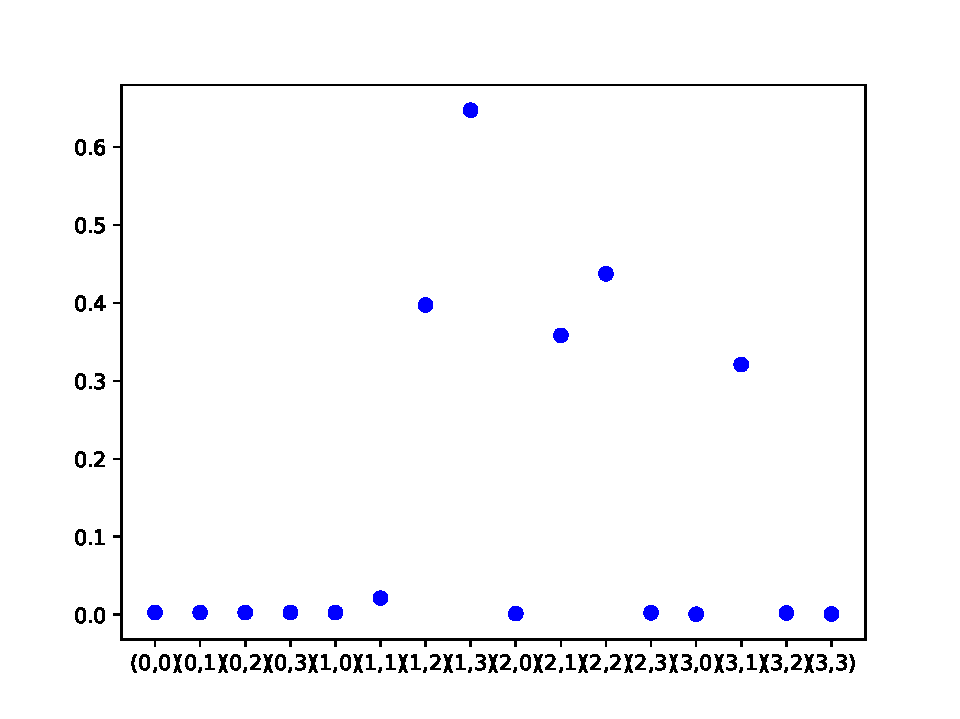
\includegraphics[width=\linewidth]{../Evolution/N=3,T=10.pdf}
  \caption{$T=10$}
\end{subfigure}%
\begin{subfigure}{.5\textwidth}
  \centering
  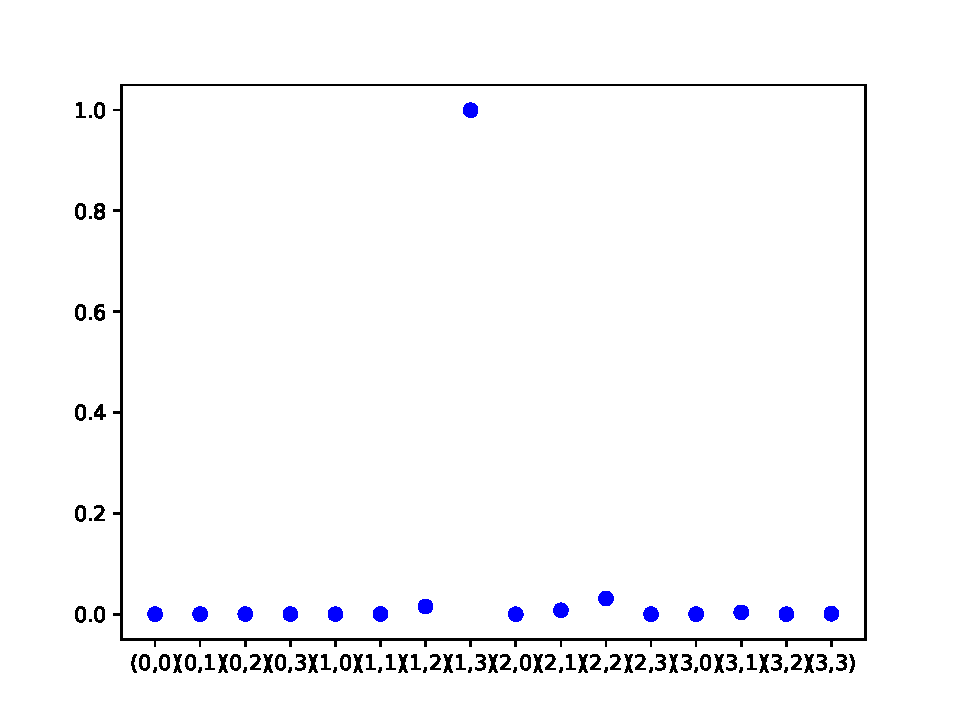
\includegraphics[width=\linewidth]{../Evolution/N=3,T=100.pdf}
  \caption{$T=100$}
\end{subfigure}\\
\begin{subfigure}{.5\textwidth}
  \centering
  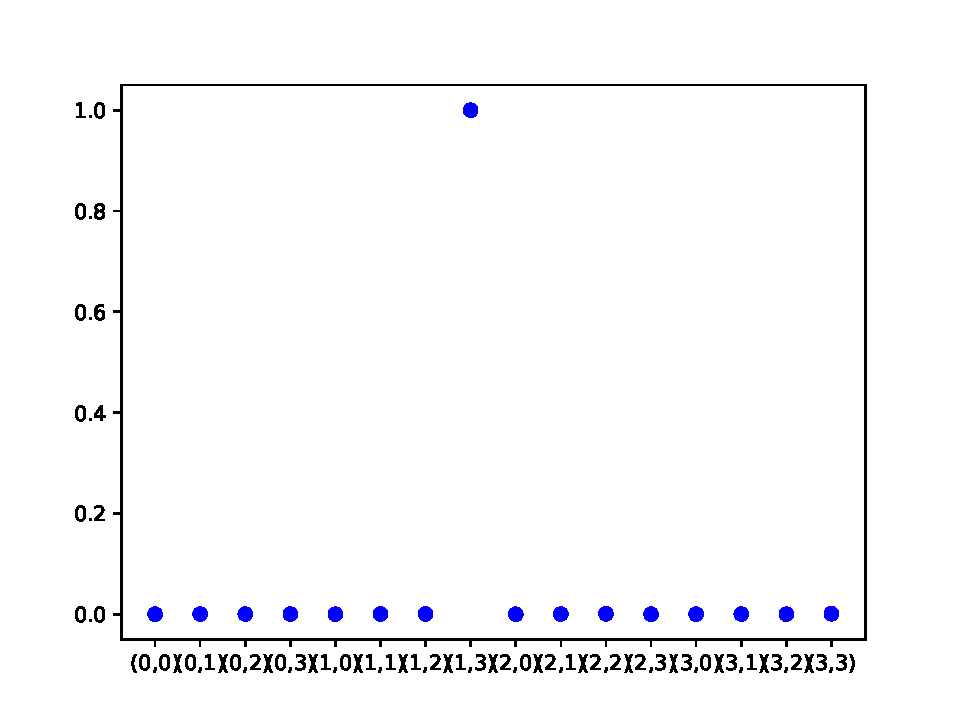
\includegraphics[width=\linewidth]{../Evolution/N=3,T=1000.pdf}
  \caption{$T=1000$}
\end{subfigure}%
\begin{subfigure}{.5\textwidth}
  \centering
  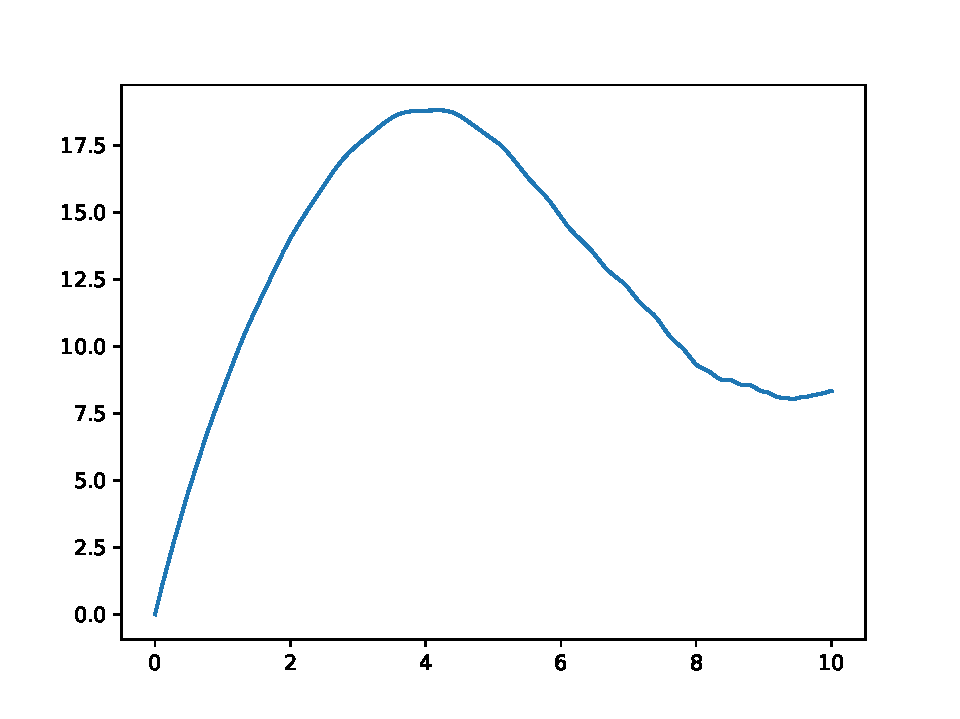
\includegraphics[width=\linewidth]{../Evolution/N=3,T=10_energies.pdf}
  \caption{Evolución de la energía para $T=10$}
\end{subfigure}\\
\begin{subfigure}{.5\textwidth}
  \centering
  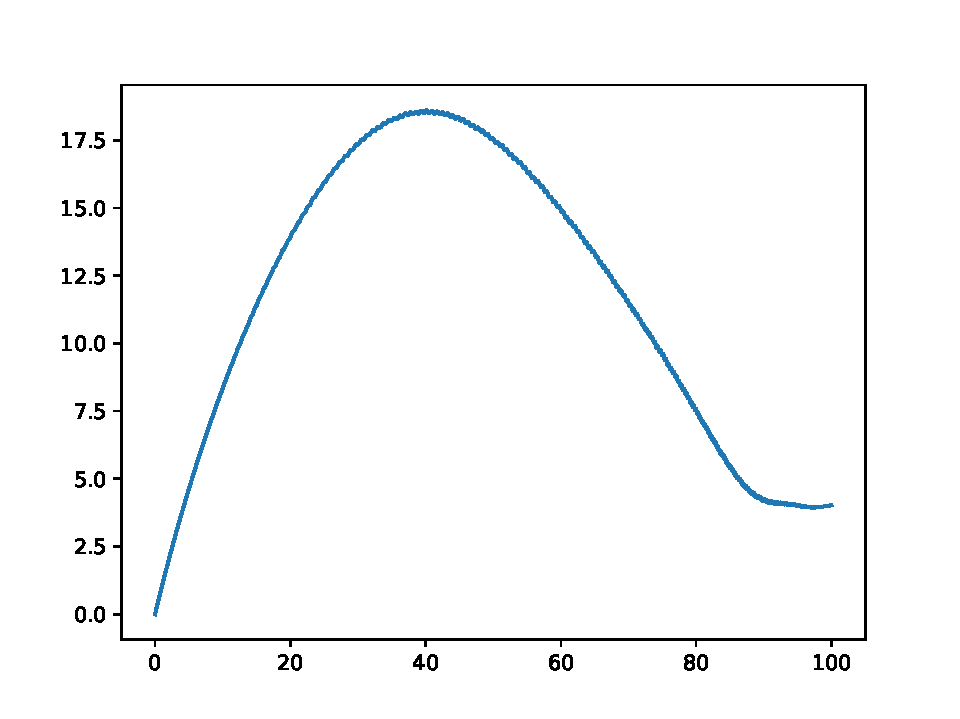
\includegraphics[width=\linewidth]{../Evolution/N=3,T=100_energies.pdf}
  \caption{Evolución de la energía para $T=100$}
\end{subfigure}%
\begin{subfigure}{.5\textwidth}
  \centering
  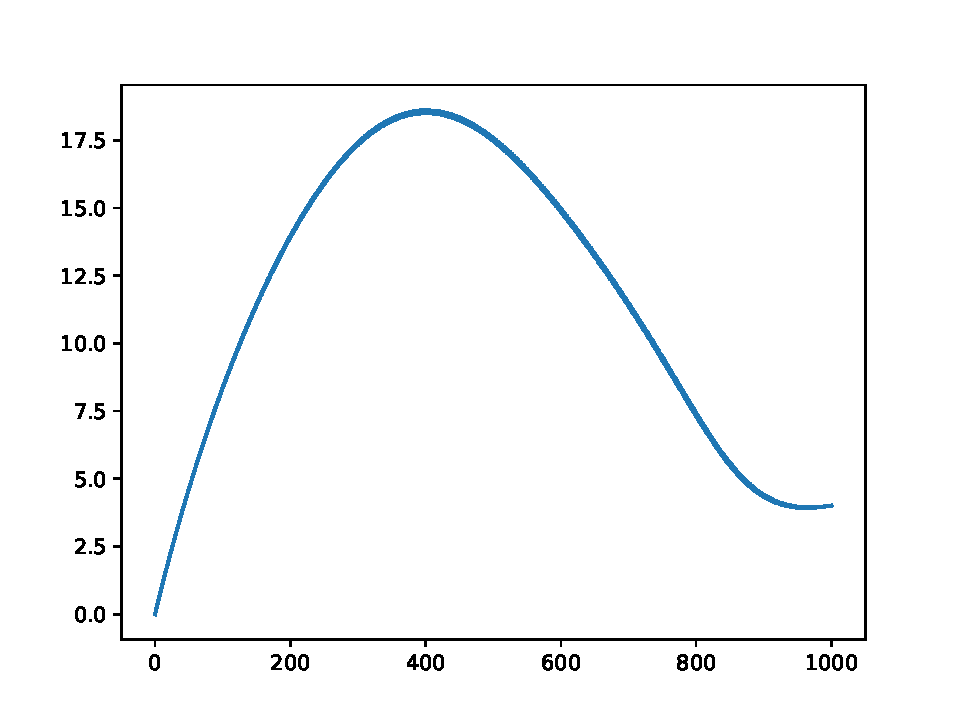
\includegraphics[width=\linewidth]{../Evolution/N=3,T=1000_energies.pdf}
  \caption{Evolución de la energía para $T=1\, 000$}
\end{subfigure}
\caption{Estado de superposición para cada qubit solución con cada índice $k$ numerado tal que $k\sim(k\ \mathbf{div}\ 2^n,k\ \mathbf{mod}\ 2^n)$ y valor de la energía para distintos rangos de integración en el caso $N=3$, $\Omega=10^{-3}$.}\label{FigRes}
\end{figure}
 

\section{Simulando la Evolución Adiabática con Circuitos}

\begin{equation}
U'_j(T)=e^{-i(T/r)\hat{H}'_r}\cdots e^{-i(T/r)\hat{H}'_1}
\end{equation}

\begin{equation}
U'_j:=e^{-iT/r(1-j/r)\hat{H}_0-iT/r\, j/r\hat{H}_f}
\end{equation}

\begin{yellowBox}
\begin{teo} [Teorema de Campbell-Baker-Hausdorff. \cite{bhatia2013matrix}\index{Teorema de Campbell-Baker-Hausdorff}]
Sean $A$ y $B$ matrices unitarias, entonces\footnotemark{} 
\begin{equation}
\norm{e^{A+B}-e^Ae^B}_2\in O(\norm{AB}_2)
\end{equation}
\end{teo}
\end{yellowBox}

\footnotetext{Se sigue de la fórmula de Campbell-Baker-Hausdorff en la que, usando el conmutador $[A,B]=AB-BA$, se tiene
\begin{equation}
e^Ae^B=e^{A+B+[A,B]/2+[X,[X,Y]]/12+\cdots}
\end{equation}
}

\begin{equation}
U''_j=e^{-iT/r(1-j/r)\hat{H}_0}e^{-iT/r\, j/r \hat{H}_f}
\end{equation}

\begin{equation}
H''_j=\mathbb{H}^{\otimes 2n}F_{0,j}\mathbb{H}^{\otimes 2n}F_{f,j}
\end{equation}

donde 

\begin{equation}
\begin{split}
F_{0,j}\ket{z} &= e^{-iT/r(1-j/r) h(z)}\ket{z}\\
F_{f,j}\ket{z} &= e^{-iT/r(j/r) f(z)}\ket{z}
\end{split}
\end{equation}


\begin{yellowBox}
\begin{teo} Sean $\hat{H}_0$ y $\hat{H}_f$ los hamiltonianos iniciales y finales para el cómputo adiabático y $f\in O(n^d)$, entonces la transformación unitaria $U(T)$ inducida por el hamiltoniano $\hat{H}(s)=\Big(1-\frac{t}{T}\Big)\hat{H}_0+\frac{t}{T}\hat{H}_f$ dependiente del tiempo puede aproximarse mediante $r$ puertas cuánticas consecutivas $U''_1,\cdots,U''_r$ con $r\in O(T^2n^{d+1})$. Además cada $U''_j$ tiene la forma $\mathbb{H}^{\otimes 2n}F_{0,j}\mathbb{H}^{\otimes 2n}F_{f,j}$ y puede implementarse eficientemente en tiempo $poly(nT)$.
\end{teo}
\end{yellowBox}

\section{Relacionando Ambos Métodos}
\subsection{Caracterización de la Complejidad}

\chapter{Conclusiones y Vías Futuras.}

%\bibliographystyle{plainurl}
%\bibliographystyle{acmlarge}
%\bibliographystyle{ACM-Reference-Format-Journals}

\begin{appendices}

%\section*{Resumen de los apéndices que se pueden encontrar en este trabajo} 

\chapter[Postulados de la Mecánica Cuántica]{Postulados de la Mecánica Cuántica\raisebox{.3\baselineskip}{\normalsize\footnotemark}}\label{Postulados}
\index{Postulados de la Física Cuántica}

\footnotetext{Recomendamos leer esta sección una vez se esté familiarizado con la introducción del capítulo \ref{chap:qubits}, pues en el caso contrario, la cantidad de información que aquí se presenta puede confundir al lector dado que usamos notación y conceptos que se introducen en dicho capítulo.}

Presentamos en esta sección una colección de postulados básicos de la mecánica cuántica. Dependiendo de la fuente que se consulte, estos postulados pueden variar desde cuatro hasta siete o más postulados. La formulación axiomática de la teoría fue formalizada de forma temprana por el matemático John Von Neuman \small{\cite{von2018mathematical}}, aunque sus postulados incluían ciertas referencias a la dinámica de los sistemas que no será relevante en este trabajo, por lo que nos limitaremos a tres de los cuatro postulados más fundamentales para la teoría de la computación expuestos en \small{\cite{nielsen2002quantum}} junto a una selección de tres más extraídos de \small{\cite{postus}}.

\begin{postu}[\textbf{Principio de superposición}]\index{Principio de superposición}\label{post:hilbert} Cualquier sistema físico se puede considerar como un vector en un espacio de Hilbert $\mathcal{H}$, el cual denotamos como \emph{espacio de estados}. El sistema queda descrito en su totalidad por este vector, que es unitario en el espacio de estados.
\end{postu}

Algunos textos no incluyen en su definición de estado la condición de que sea unitario, a cambio de establecer una relación de equivalencia $\sim$ bajo la cual dos estados son equivalentes si uno es múltiplo del otro por un escalar, y trabajan sobre el espacio cociente $\bigslant{\mathcal{H}}{\sim}$.

\begin{postu}[\textbf{Evolución temportal determinista}]\label{post:evol}La evolución de un sistema cuántico cerrado viene determinada por un operador lineal unitario. Usando el término <<hamiltoniano>>\index{Hamiltoniano} y la notación $\hat{H}$ para tal operador y la notación $\ket{\phi(t)}$ para el estado del sistema en el instante $t$, entonces la evolución temporal viene dada por la ecuación diferencial de Schrödinger\index{Ecuación de Schrödinger}

\begin{equation}
i\hbar\frac{\partial}{\partial t}\ket{\phi(t)}=\hat{H}\ket{\phi(t)}
\end{equation}

donde $\hbar$ es la conocida como constante de Planck normalizada\index{Constante de Planck $\hbar$} $\hbar=\frac{h}{2\pi}$, cuyo valor es aproximadamente $1.054571\cdot 10^{-34}$ julios por segundo. Si el hamiltoniano no es constante en el tiempo y queremos enfatizarlo podremos escribir

\begin{equation}
i\hbar\frac{\partial}{\partial t}\ket{\phi(t)}=\hat{H}(t)\ket{\phi(t)}
\end{equation}

\end{postu}

\begin{obs}
El lector puede haberse dado cuenta de que usamos la notación $\partial/\partial t$ para la derivada parcial en vez de la clásica  $d/dt$ para funciones de una sola variable. Esto simplemente lo hacemos por una consistencia notacional e histórica con la teoría más general, pues en la teoría cuántica más allá de la rama computacional un estado $\ket{\phi(t)}$ hace referencia a una entidad más general: una onda. Por esto podríamos ver el estado $\ket{\phi(t)}$ como una función $\phi(t,\vec{r})$ que asocia a cada punto $\vec{r}$ del espacio y cada instante $t$, un valor complejo, lo que justifica que usemos la notación multivariable y la derivada parcial. Sin embargo, como esta interpretación ondulatoria de los estados cuánticos no es necesaria para nuestro trabajo, usaremos en lo que respecta a las secciones en las que usemos la evolución de Schrödinger la notación $d/dt$.
\end{obs}

\begin{ejs}
El hamiltoniano para una partícula cuántica libre de masa $m$ no sujeta a fuerzas externas moviéndose en una dimensión viene definido por
\begin{equation}
\hat{H}=-\frac{\hbar^2}{2m}\frac{\partial^2}{\partial x^2}
\end{equation}

y si suponemos que la partícula está sujeta al campo potencial de una fuerza conservativa $V(x)$ el hamiltoniano será

\begin{equation}
\hat{H}=-\frac{\hbar^2}{2m}\frac{\partial^2}{\partial x^2}+V(x)
\end{equation}

que es la forma más común en la que podemos encontrarlo en la literatura.
\end{ejs}

\begin{postu}[\textbf{Sistemas compuestos}] \label{post:4}El espacio de estados de un sistema compuesto es el producto tensorial de los espacios correspondientes a cada uno de los estados componentes del sistema. 
\end{postu}

\begin{postu}[\textbf{Caracterización de las mediciones}] \label{post:5}Los únicos resultados posibles de una magnitud $A$ (que llamaremos <<observable>>) de un sistema cuántico son los autovalores del operador asociado $\hat{A}$.
\end{postu}

Podemos ver un ejemplo de este postulado como sigue: para una partícula libre podemos considerar su energía cinética $K$. Sea $\hat{K}$ el operador que dado un estado cuántico para la partícula encapsula su energía cinética, tal operador viene dado por

\begin{equation}
\hat{K}=-\frac{\hbar^2}{2m}\frac{\partial^2}{\partial x^2}
\end{equation}

que, como es sencillo comprobar, es lineal y unitario.

\begin{postu}[\textbf{Caracterización probabilista de la medición}] \label{post:6} Cuando se realiza una medida de un observable A sobre un estado $\ket{\phi}$, la probabilidad de obtener un autovalor\index{Autovalor} $a_n$ viene dada por la magnitud $|\bra{a_n}\ket{\phi}|^2$.
\end{postu}

Siguiendo el ejemplo anterior, si el operador $\hat{K}$ tiene autoestados\index{Autoestado} $\{\ket{k_i}\}_{i\in I}$ con autovalores $\{k_i\}_{i\in I}$, la partícula en el estado $\ket{\phi}$ solo podrá tomar valores de energía cinética $\{k_i\}_{i\in I}$. Cada uno de ellos con probabilidad $|\bra{k_i}\ket{\phi}|^2$.

\begin{postu}[\textbf{Reducción de un estado cuántico}] \label{post:7} Si la medición de un observable $A$ ha devuelto un autovalor $a_n$, el estado del sistema tras la medición será $\ket{a_n}$. 
\end{postu}

Y si al medir la energía cinética de la partícula hemos obtenido un autovalor para la energía cinética $k_i$ entonces el estado de la partícula será $\ket{k_i}$.

\chapter{Aspectos de la Computación Cuántica}

\section{Circuitos Universales}\label{sec.univ}

Tal y como en computación clásica las puertas NAND proporcionan una puerta universal que basta para construir cualquier circuito booleano (se puede demostrar que cualquier otra puerta lógica booleana se puede construir con un número finito de puertas NAND), en computación cuántica ocurre algo similar. Ya en la década de los años 90 se comenzó a estudiar \cite{1995PhRvA..52.3457B} qué conjuntos de puertas eran suficientes para construir cualquier circuito cuántico. De hecho se puede demostrar que hay un gran número de bases universales, algunas de ellas se muestran en \cite{brylinski2002universal}, nosotros aquí daremos un conjunto que consideramos el más importante pues está formado por tres (veremos posteriormente que tan solo dos) puertas cuánticas extremadamente comunes.\\

\begin{defin}[Conjunto universal] Un conjunto finito de puertas cuánticas se dice universal si cualquier operador unitario puede aproximarse con precisión arbitraria por un circuito cuántico finito que solamente contiene puertas del conjunto.
\end{defin} \index{Circuito universal}

La razón de que se defina la aproximación con un error arbitrario es que la cantidad de posibles puertas cuánticas unitarias es no numerable y la cantidad de circuitos finitos usando una puertas de un conjunto finito es numerable, así pues en general no podremos aproximar excepto por un error arbitrario\footnotemark{}.	\\

Para cuantificar el error aquí contemplado solamente se requiere una norma definida en el espacio de las matrices complejas que denotaremos $\mathcal{M}_{N\times N}(\mathbb{C})$, sin embargo la norma que definamos es irrelevante dado que en un espacio de dimensión finita todas las normas son equivalentes (\cite{kreyszig1978introductory}), y por tanto no difieren en más de una constante multiplicativa estrictamente positiva. Usando la norma infinito $\norm{\cdot}_\infty $ componente a componente, o como es más conocida, la norma \emph{entrywise}, que consiste en identificar $\mathcal{M}_{N\times N}(\mathbb{C})$ con $\mathbb{C}^{N^2}$  podemos escribir el siguiente teorema, publicado por primera vez en \cite{deutsch1989quantum}. \\

\footnotetext{Por esta misma razón ciertos textos como \cite{2004cs........9051T} distinguen entre \emph{conjuntos universale}s, los cuales podrían aproximar exactamente cualquier puerta cuántica pero que, necesariamente, serían infinitos y los \emph{conjuntos aproximadamente universales} que corresponderían a la definición que aquí se ha realizado.}

\begin{purpleBox}
\begin{teo}[$\{H, R_s, CCNOT\}$ es universal.]\label{teoUniv}
Para cada $D\geq 3$ y $\varepsilon > 0$ existe un $l\geq (D\log \frac{1}{\varepsilon})^3$ tal que se cumple lo siguiente:\\

Cada matriz unitaria $U\in\mathcal{M}_{D\times D}(\mathbb{C})$ puede ser aproximada por un producto de matrices unitarias $U_1,\cdots,U_l$ de forma que si $(i,j)$ son números menores o iguales que $D$ se satisface
\begin{equation}
\Big| U_{i,j}-(U_l\cdots U_1)_{i,j} \Big| < \varepsilon
\end{equation} 
y cada $U_r$ corresponde a aplicar la puerta Hadamard $H$, la puerta Toffoli o la puerta de desplazamiento de fase en, como máximo, tres qubits.
\end{teo}
\end{purpleBox}

De hecho, tal y como se demostró en el artículo \cite{2002quant.ph..5115S} y en \cite{2003quant.ph..1040A}, las puertas de Hadamard y Toffoli bastan. Esto es debido a la mencionada observación \ref{ObservacionEfectosObservables} por la cual podemos despreciar los desplazamientos de fase compleja común a los coeficientes de una superposición.\\

%\subsection{Computación probabilista vs computación cuántica.}

\begin{defin}Se dice que un circuito $C$ tiene tamaño $n$ con respecto a un conjunto $\mathcal{U}$ de puertas universales si $n$ puertas cuánticas de $\mathcal{U}$ son necesarias para implementar el circuito.
\end{defin} \index{Tamaño circuital}


\section{Principio de No Clonación}\label{NC}

Vemos en este punto una de las particularidades más llamativas e importantes de la computación cuántica: \textbf{la información no se puede duplicar}. El teorema que mostramos a continuación, universalmente cierto, implica la imposibilidad de clonar un estado cualquiera en un registro arbitrario. Este hecho es importante pues dado que se pudiese clonar un estado un número arbitrario de veces podríamos, con medios técnicos ilimitados, obtener una precisión arbitraria de un estado cuántico (excepto, por la observación \ref{ObservacionEfectosObservables}, desplazamientos de fase comunes) simplemente clonando el estado y realizando mediciones. De esta forma, podríamos establecer un muestreo probabilístico de los valores obtenidos en las mediciones y obtener de forma arbitrariamente precisa el estado original.\\

\begin{purpleBox}
\begin{teo}[Teorema de no clonación \cite{QuantumWhaley}] \index{Teorema de no clonación}
No existe ningún operador unitario $U$ en un espacio producto $H\times H$ de un espacio de Hilbert $H$ tal que para un estado normalizado cualquiera  $\ket{\phi}$ en $H$ se cumpla que
\begin{equation}
U(\ket{\phi}\ket{0})=e^{i\alpha(\phi,0)}\ket{\phi}\ket{\phi}
\end{equation}
\end{teo}
\end{purpleBox}

\begin{proof}
Procedemos por reducción al absurdo. Consideremos que existe una puerta $U$ como la mencionada, entonces se tiene que
\begin{equation}
\begin{split}
\bra{\phi}\ket{\psi}\bra{0}\ket{0}&=\bra{\phi}\bra{0}\ket{\psi}\ket{0}=\bra{\phi}\bra{0} U^\dag U\ket{\psi}\ket{0} \\
&=e^{-i(\alpha(\phi,0)-\alpha(\psi,0))}\bra{\phi}\bra{\phi}\text{Id}\ket{\psi}\ket{\psi}\\
&=e^{-i(\alpha(\phi,0)-\alpha(\psi,0))}\bra{\phi}\ket{\psi}^2
\end{split}
\end{equation}

Como $\ket{0}$ es un estado normalizado, $\bra{0}\ket{0}=1$ y por tanto $|\bra{\phi}\ket{\psi}|=|\bra{\phi}\ket{\psi}|^2$ (pues $|e^{-i(\alpha(\phi,0)-\alpha(\psi,0))}|=1$). Esto implica que $|\bra{\phi}\ket{\psi}|=0$ o bien $|\bra{\phi}\ket{\psi}|=1$. Así, la desigualdad de Cauchy–Bunyakovsky–Schwarz implica que $\phi=e^{i\beta}\psi$ o bien que $\phi$ y $\psi$ son ortogonales. Lo que, obviamente, no se da para cualquier $\ket{\phi}$ y $\ket{\psi}$ arbitrario, por lo que \textbf{un operador unitario $U$ no puede clonar de forma general un estado cuántico}.
\end{proof}

\begin{nota}
Una consecuencia interesante de la demostración anterior es que un computador cuántico \textbf{sí} puede clonar de forma general un registro clásico. Es decir si tenemos un estado $\ket{i}$ con $i\in{0,1}$, se puede realizar sin ningún tipo de problema la operación cuántica $\ket{i}\ket{0}\rightarrow\ket{i}\ket{i}$. De hecho usaremos este tipo de operaciones más adelante en este trabajo.
\end{nota}

Podemos mencionar que existe un análogo inverso al Teorema de la No Clonación llamado el Teorema de No Borrado\footnote{No deleting theorem.} que se puede enunciar como sigue

\begin{nota}[Teorema de No Borrado, \cite{2000Natur.404..164K}]\index{Teorema de no borrado} No existe ningún operador cuántico unitario $U$ tal que, en general, se tenga que

\begin{equation}
U(\ket{\phi}\ket{\phi}\ket{A})=\ket{\phi}\ket{0}\ket{A'}
\end{equation}
\end{nota}

\section{Teleportación Cuántica}\label{sdc}\index{Codificación superdensa}

\begin{center}
\red{Hay una inconsistencia narrativa en esta sección? Importa?}
\end{center}

Veamos en este punto, y usando como medio una situación hipotética, cómo podremos, en condiciones especiales, transmitir un qubit cuántico usando solamente una pequeña cantidad de información clásica.\\

Supongamos que dos astrounautas llamadas, sin mucha originalidad, Alicia y Belén se encuentran en puntos distintos del sistema solar. Una de ellas, digamos que Alicia, quiere enviar la información del estado de un qubit que ella tiene en posesión a Belén, pero con la restricción de que su agencia espacial solo permite el envío de información clásica, pues los sistemas de comunicación cuántica no están todavía suficientemente desarrollados. Lo primero que Alicia podría pensar es en intentar mandar la información del estado completamente de forma clásica pero en este punto se encuentra dos problemas fundamentales:
\begin{itemize}
\item Alicia no puede saber en qué estado se encuentra el qubit dado que, como hemos visto, solo puede efectuar una única medición y no puede acceder al contenido de la superposición del qubit.
\item Si pudiese, la situación no sería ciertamente mejor. Pues tendría que enviar a Belén una cantidad \emph{infinita} de información para poder transmitir un estado en un rango continuo con total precisión.
\end{itemize}

En este punto Alicia recuerda que en sus años de formación en La Tierra, ellas crearon un par EPR $\ket{\mathbf{\Phi}^+}$, quedándose cada una con uno de los qubits del par. Esperando que Belén aún tenga el suyo consigo, Alicia idea una forma de transmitirle información.\\

Imaginemos que el qubit que Alicia quiere transmitir es $\ket{\phi}$. La idea será la siguiente: Alicia interactuará con su qubit del par EPR común mediante un circuito cuántico que se puede visualizar en la figura \ref{teleportation}. La medición tras la aplicación del circuito devolverá a Alicia un valor en $\{00,01,10,11\}$. La principal sorpresa será que Belén, usando simplemente este valor medido (2 bits) puede recuperar completamente el estado $\ket{\phi}$.\footnote{Este hecho no contradice el principio de no clonación que hemos mostrado, puesto que en ningún momento se clona información. Debido a que el qubit original se destruye al medirlo, y esto ocurre antes de que el nuevo qubit se genere en la estación espacial de Belén, en ningún momento existen dos copias idénticas del estado $\ket{\varphi}$ simultáneas.}\\

Supongamos que queremos enviar (teleportar) el qubit en el estado arbitrario $\ket{\phi}=\alpha\ket{0}+\beta\ket{1}$. Si suponemos que los tres qubits forman un registro (Alicia obviamente no podrá interactuar con el qubit del par EPR de Belén, pero conceptualmente nada nos impide considerar el qubit de Belén como parte del sistema, siempre que no realicemos ninguna operación sobre él) y si llamamos $\ket{\varphi_0}=\ket{\varphi}\ket{\mathbf{\Phi}^+}$ al registro inicial, usando la definición explícita que conocemos del par EPR obtenemos

\begin{equation}
\ket{\varphi_0}=\frac{1}{\sqrt{2}}\Big(\alpha\ket{0}(\ket{00}+\ket{11})+\beta\ket{1}(\ket{00}+\ket{11})\Big)
\end{equation} 

Cuando Alicia aplica la puerta CNOT sobre sus dos qubits como se aprecia en la figura \ref{teleportation} el estado cambia a 

\begin{equation}
\ket{\varphi_1}=\frac{1}{\sqrt{2}}\Big(\alpha\ket{0}(\ket{00}+\ket{11})+\beta\ket{1}(\ket{10}+\ket{01})\Big)
\end{equation} 

Si aplicamos en este punto la puerta de Hadamard únicamente al primer qubit podemos obtener el estado 

\begin{equation}
\ket{\varphi_2}=\frac{1}{2}\Big(\alpha(\ket{0}+\ket{1})(\ket{00}+\ket{11})+\beta(\ket{0}-\ket{1})(\ket{10}+\ket{01})\Big)
\end{equation}

Además, reagrupando términos, podemos ver el estado anterior fácilmente como 


\begin{equation}\label{myEqTmp}
\ket{\varphi_2}=\frac{1}{2}\Big(\ket{00}(\alpha\ket{0}+\beta\ket{1})+\ket{01}(\alpha\ket{1}+\beta\ket{0})+\ket{10}(\alpha\ket{0}-\beta\ket{1})+\ket{00}(\alpha\ket{1}-\beta\ket{0}) \Big)
\end{equation}

Escribiendo el estado de tal forma podemos ver que si Alicia mide sus dos qubits y obtiene un valor de $\{00,01,10,11\}$ concreto entonces el estado del qubit de Belén queda unívocamente definido. Por ejemplo, si Alicia obtiene el valor $01$ al medir el qubit entonces por la ecuación \ref{myEqTmp} el valor del qubit de Belén debe ser $\alpha\ket{1}+\beta\ket{0}$. Así pues, Belén podría obtener el qubit original $\ket{\varphi}$ simplemente aplicando un operador a su registro. Por tanto toda la información que necesitamos transferir es 2 bits para transmitir un valor teóricamente infinito de información.\footnotemark{}\\

\footnotetext{Esta afirmación requeriría un estudio mucho más detallado sobre el significado del término <<información>>. Si asumimos la definición clásica de la información como disminución de la incertidumbre, habría que preguntarse entonces cuánta incertidumbre es capaz de producir un qubit asumiendo que tenemos restricciones de extracción de la información por el colapso por medición. Dejamos tal tema de estudio a los teóricos de la información cuántica.}

Supongamos que $\ket{\theta}$ es el estado del qubit de Belén tras la ejecución del circuito de Alicia y $M_1$ y $M_2$ los valores medidos y enviados a Belén, entonces el qubit original $\ket{\varphi}$ viene dado por

\begin{equation}
\ket{\varphi}=\begin{cases}
\ket{\theta}\qquad  &\text{ si } M_1=0,\ M_2=0 \\
X\ket{\theta}\qquad  &\text{ si } M_1=0,\ M_2=1 \\
Z\ket{\theta}\qquad  &\text{ si } M_1=1,\ M_2=0 \\
ZX\ket{\theta}\qquad  &\text{ si } M_1=1,\ M_2=1
\end{cases}
\end{equation}

Lo que podemos escribir más compactamente usando que la potencia nula de una matriz es la identidad como

\begin{equation}
\ket{\varphi}=Z^{M_1}X^{M_2}\ket{\theta}
\end{equation}

Este mecanismo de codificación del estado completo de un qubit completo en tan solo dos bits clásicos se conoce comúnmente como \emph{codificación superdensa} o, en inglés, \emph{superdense coding}. Aunque esta particularidad cuántica se conocía desde 1935, la comunidad científica era escéptica al hecho de que realmente fuese posible que un cambio en un sistema cuántico pudiese tener efectos instantáneos en otro independientemente de la distancia que los separase pues esto parecía violar las leyes de causalidad de la Relatividad General de Einstein transmitiendo información más rápido que la propia luz, lo cual el propio Einstein denominó como la <<acción fantasmal a distancia>>\footnote{Spooky action at a distance.} en un sentido claramente peyorativo, y dicha situación pasó a conocerse como la Paradoja Einstein-Podolsky-Rosen\footnote{Abreviadamente <<Paradoja EPR>>}. Análisis rigurosos posteriores propusieron que en realidad no había una violación del postulado de localidad de la Relatividad dado que se necesitaba el envío de los dos bits de forma clásica, de hecho, esto pasó a conocerse como el Teorema de la No Comunicación\footnote{No-communication Theorem. } (\cite{Peres:2002wx}, sección 2.E.). Fue entonces, en 1993 cuando en \cite{Bennett93teleportingan} se propuso la idea que hemos mencionado para la codificación superdensa abriendo una puerta a las comprobaciones experimentales de esta acción a distancia.\\

En 1998, investigadores del Caltech junto a institutos europeos consiguieron teleportar el primer estado de un fotón constituyendo así la teleportación como una realidad física. Durante todos los años siguientes se realizaron mayores experimentos, por ejemplo, se consiguió realizar una teleportación instantánea a 97km de distancia (\cite{2012Natur.488..185Y}) incluso teleportación mediante fibra óptica a 25km de distancia (\cite{2014NaPho...8..775B}). El récord a día de hoy lo ostenta un grupo de científicos chinos de diferentes universidades que consiguió teleportar en \cite{2017Natur.549...70R} el estado de un fotón a 1400km de distancia, desde el Tibet hasta un satélite en órbita.\\

\begin{figure}
\begin{center}
\includegraphics[scale=1.2,frame]{../Diagramas/CircuitTeleportation.pdf}
\end{center}
\caption{Circuito cuántico para la realización de la teleportación.}\label{teleportation}
\end{figure}

\chapter{Resultados de Aritmética Elemental}

\begin{defin}[Grupo]\index{Grupo}
Un \textbf{grupo} $(G,\cdot)$ es un conjunto $G$ junto a una operación interna $(\cdot):G\times G \rightarrow G$ asociativa, con neutro y con simétrico para cada elemento.
\end{defin}

\begin{defin}[Subgrupo]\index{Subgrupo} Un grupo $(H,\cdot_H)$ se dice un \textbf{subgrupo} de un grupo $(G,\cdot)$ si $H\subseteq G$ y $\cdot_H=\cdot|_H$, es decir, $\cdot_H$ es la operación heredada de $G$ aplicada sobre el subconjunto $H$.
\end{defin}

\begin{defin} \index{El grupo aditivo $\mathbb{Z}_m$}
Denotaremos como $\mathbb{Z}_m$ al conjunto de números enteros $1\leq i\leq m$.  Este conjunto será un grupo $(\mathbb{Z}_m, +)$ junto la operación $+$ suma módulo $m$.
\end{defin}

\begin{defin} \index{El grupo multiplicativo $\mathbb{Z}_m^*$} \label{apend:algebra}
Denotaremos como $\mathbb{Z}_m^*$ al conjunto de números enteros $1\leq i\leq m$ tal que $m$ es coprimo con $i$, es decir $mcd(i,m)=1$. Este conjunto será un grupo $(\mathbb{Z}_m^*, \cdot)$ junto la operación $\cdot$ producto módulo $m$.

Definiremos, para cada $r\in\mathbb{Z}_m$ el conjunto $r\mathbb{Z}_m^*\subseteq\mathbb{Z}_m $ como el conjunto de los elementos $rx$ con $x\in\mathbb{Z}_m^*$. Es sencillo comprobar que 
\begin{equation}
r\mathbb{Z}_m^*=\mathbb{Z}_m^*\quad \Leftrightarrow \quad r\in\mathbb{Z}_m^* \quad \Leftrightarrow \quad mcd(m,r)=1
\end{equation}

\end{defin}

\begin{defin}[Función $\phi$ de Euler]\index{Función $\phi$ de Euler}\label{Euler}
Definimos la función $\phi$ de Euler de un número $r$ como el número de elementos menores que el propio $r$ coprimos con él mismo. Es decir, $\phi(r)=|\mathbb{Z}_r^*|$.\\

De hecho la función de Euler tiene una forma explícita relativamente sencilla basada en la descomposición prima del propio $r$, aunque no la daremos por no ser relevante en el presente trabajo. 
\end{defin}

\begin{prop}\label{otromas} Si $G$ es un grupo conmutativo y $g=g_1\cdots g_n\in G$ entonces $o(g)\, =\, mcm(o(g_1),\cdots,o(g_n))$.
\end{prop}

\begin{defin}[Isomorfismo] \index{Isomorfismo de grupos} Una función $f:(G,\cdot_G)\rightarrow(G'.\cdot_{G'})$ se dice un \textbf{isomorfismo de grupos} si
\begin{itemize}
\item $f$ es biyectiva. ($f$ es suprayectiva e inyectiva).
\item $f(a\cdot_Gb)=f(a)\cdot_{G'}f(b)\ \forall\ a,b\in G $
\end{itemize}

\end{defin}

\begin{defin}[Orden] \index{Orden (grupo)}
Definimos el \textbf{orden de un elemento} $g\in G$ como el mínimo $n>0$ tal que $g^n=1$, donde $1$ es el elemento unidad de $G$. Análogamente definimos el \textbf{orden de un grupo} $G$ como su cardinalidad, es decir, el número de elementos distintos que contiene. A este número lo denotaremos $o(g)$.
\end{defin}

\begin{prop} \label{otroTeoremaNumeros} Sea $G$ un grupo y $g\in G$. Si $o(g)=r$ entonces la secuencia $\{1,g,g^2,\cdots,g^{r-1}\}$ no contiene ninguna repetición.
\end{prop}

\begin{teo}[Teorema Chino de los Restos]\index{Teorema Chino de los Restos}\label{teoChino}
Sean $I_1,\cdots,I_n$ ideales de un anillo $R$ tales que para todo $i\neq j$, $I_i+I_j=R$ entonces existe un isomorfismo
\begin{equation}
f:R/(I_1\cap\cdots\cap I_n)\rightarrow R/I_1\times\cdots\times R/I_n
\end{equation}
\end{teo}

\begin{corol}[Teorema Chino de los Restos, versión entera]\label{teoChinoEnt}
Sean $n_1,\cdots,n_k$ enteros coprimos dos a dos, entonces dados $k$ enteros $a_1,\cdots,a_k$ existe un entero $x$ que resuelve el sistema de congruencias
\begin{equation}
\systeme*{x \equiv a_1\ (\text{mod } n_1),x \equiv a_2\ (\text{mod } n_2),\vdots \hspace{2.07cm},x \equiv a_k\ (\text{mod } n_k)}
\end{equation}

\end{corol}

\begin{lema}\label{probPar}
Sea $n$ impar, al menos la mitad de los elementos de $(\mathbb{Z}/n\mathbb{Z})^*=\mathbb{Z}_n^*$ tienen orden par.
\end{lema}

\begin{proof}
Supongamos que tenemos un $x$ con orden impar $r$. Entonces
\begin{equation}
(-x)^r=(-1)^rx^r=-1
\end{equation}

Lo que implica que el orden de $-x$ es $2r$ que es par. Por lo tanto al menos la mitad de elementos en $\mathbb{Z}_n^*$ tienen orden par.
\end{proof}

\begin{teo}[Algoritmo de Euclides, \cite{shoup2009computational}] Sean $a,b$ pertenecientes a un dominio euclideo (en particular, a $\mathbb{Z}$) podemos obtener un máximo común divisor de $a$ y $b$ mediante el algoritmo\footnote{De hecho, se puede ver de nuevo que este algoritmo se ejecuta en tiempo polilogarítmico.} siguiente
\begin{megaalgorithm}
\caption{Algoritmo de Euclides}\label{euclidesAlg}\index{Algoritmo de Euclides}
\begin{algorithmic}[1]
\Procedure{mcd}{$a,b$: enteros}
\State $r_0 \gets a$
\State $r_1 \gets b$
\State $i \gets 1$
\While{\texttt{$r_i\neq 0$}}
\State $r_{i+1}\gets r_{i-1} \text{ mod } r_i$
\State $i \gets i+1$
\EndWhile
\Return $r_{i-1}$
\EndProcedure
\end{algorithmic}
\end{megaalgorithm}
\end{teo}

%\chapter{Complejidad clásica.}\label{sec:Cclasica}
%
%\begin{figure}[h]
%\begin{center}
%\includegraphics[scale=1.5]{../Diagramas/Turing.pdf}
%\end{center}
%\caption{Máquina clásica de Turing}
%\end{figure}
%
%\begin{greenBox}
%\begin{defin}[Máquina de Turing]\index{Máquina de Turing clásica}
%Una \textbf{Máquina de Turing} (abreviado TM) es una hepta-tupla ordenada $(\Sigma, \lambda, Q, q_i, A, F, \delta)$ donde,
%
%\begin{itemize}
%\item $\Sigma$ es un conjunto finito, llamado el \textbf{alfabeto} de símbolos.
%\item $Q$ es un conjunto finito, llamado el conjunto de \textbf{estados}.
%\item $\lambda\in \Sigma$ es un símbolo llamado \textbf{símbolo blanco}.
%\item $q_i\in Q$ es el \textbf{estado inicial}.
%\item $A\subset Q$ es el conjunto de \textbf{estados de aceptación}.
%\item $F\subset Q$ es el conjunto de \textbf{estados finales}.
%\item $\delta: \Sigma \times Q \rightarrow \Sigma \times Q \times \{L,R\}$ es la \textbf{función de transición}.
%\end{itemize}
%\end{defin}
%\end{greenBox}
%
%\begin{figure}[h]
%\begin{center}
%\includegraphics[scale=.5]{../Diagramas/Inclusion-crop.pdf}
%\end{center}
%\caption{Diagrama de inclusión de clases de complejidad}
%\end{figure}
%
%\begin{greenBox}
%\begin{defin}[La clase $\PP$ mediante TM]
%Un lenguaje $\mathcal{L}$ pertenece a $\PP$ si y solo si existe una TM clásica (determinista) $M$ tal que
%\begin{itemize}
%\item $M$ se ejecuta en tiempo polinómico para cualquier entrada.
%\item Para cada $x\in\mathcal{L}$, $M$ devuelve $1$.
%\item Para cada $x\not\in\mathcal{L}$, $M$ devuelve $0$.
%\end{itemize}
%\end{defin}
%\end{greenBox}
%
%\begin{greenBox}
%\begin{defin}[La clase $\PP$ mediante circuitos booleanos]
%Un lenguaje $\mathcal{L}$ pertenece a $\PP$ si y solo si existe una familia uniforme de tiempo polinómico\footnote{Una familia uniforme de tiempo polinómico es una familia tal que, dado un $n$, podemos obtener una descripción de $C_n$ con una MT en tiempo polinómico.} $\{C_n\}_{n\in\mathbb{N}}$ tal que
%\begin{itemize}
%\item Para cada $n$ natural, $C_n$ toma $n$ bits de entrada y su salida consiste en un solo bit.
%\item Para cada $x\in\mathcal{L}$, $C_{|x|}(x)=1$.
%\item Para cada $x\not\in\mathcal{L}$, $C_{|x|}(x)=0$.
%\end{itemize}
%\end{defin}
%\end{greenBox}
%
%\section{Las clases de la computación probabilista}
%\index{Máquina de Turing probabilista}
%
%\begin{greenBox}
%\begin{defin}[La clase de complejidad $\BPP$]\index{Clase $\BPP$}
%Sea $T:\mathbb{N}\rightarrow\mathbb{N}$ y $\mathcal{L}\subseteq\{0,1\}^*$, decimos que una máquina de Turing probabilista $M$ decide $\mathcal{L}$ en tiempo $T(n)$ con probabilidad mqyor que $2/3$ si para cada $x\in\{0,1\}^*$, $M$ para en $T(|x|)$ pasos independientemente de sus decisiones aleatorias y $\mathbf{Pr}[M(x)=L(x)]> 2/3$.\\
%
%Sea $\BPTIME(T(n))$ la clase de los lenguajes decidibles por máquinas de Turing probabilistas en tiempo $O(T(n))$. Definimos $\BPP=\bigcup_c\BPTIME(n^c)$.\index{Clase $\BPTIME(T(n))$}
%\end{defin}
%\end{greenBox}
%
%\begin{greenBox}
%\begin{defin}[La clase de complejidad $\mathbf{PP}$]\index{Clase $\mathbf{PP}$}
%Sea $T:\mathbb{N}\rightarrow\mathbb{N}$ y $\mathcal{L}\subseteq\{0,1\}^*$, decimos que una máquina de Turing probabilista $M$ decide $\mathcal{L}$ en tiempo $T(n)$ con probabilidad mayor que $1/2$ si para cada $x\in\{0,1\}^*$, $M$ para en $T(|x|)$ pasos independientemente de sus decisiones aleatorias y $\mathbf{Pr}[M(x)=L(x)]> 1/2$.\\ \index{Clase $\PPTIME(T(n))$}
%
%Sea\footnotemark[1] $\PPTIME(T(n))$ la clase de los lenguajes decidibles por máquinas de Turing probabilistas en tiempo $O(T(n))$. Definimos $\PP=\bigcup_c\PPTIME(n^c)$.
%\end{defin}
%\end{greenBox}
%\footnotetext[1]{La notación aquí presentada para la clase $\PPTIME$ no se ha tomado de ningún texto, ya que no hemos podido encontrar referencias. La definimos, por tanto, con ese nombre como un análogo a la definición $\BPP$. Además, tal notación arbitraria no tendrá repercusión en el resto del trabajo pues únicamente usaremos la clase $\mathbf{PP}$.}
%
%Lo siguiente es inmediato.
%
%\begin{greenBox}
%\begin{prop}
%$\BQP\subseteq\mathbf{PP}$
%\end{prop}
%\end{greenBox}
%
%\begin{proof}
%Tomemos un $\mathcal{L}$ en $\BQP$. Por definición existe un natural $a$ tal que $\mathcal{L}$ es decidible por una máquina de Turing probabilista con probabilidad mayor que $2/3$ en tiempo $O(n^a)$, lo que implica que $\mathcal{L}$ también es decidible por una máquina de Turing probabilista con probabilidad mayor que $1/2$ en tiempo $O(n^a)$ y por tanto $\mathcal{L}\in \mathbf{PP}$.
%\end{proof}
%
%
%\section{La clase \texorpdfstring{$\PSPACE$}{PSPACE}}
%\begin{greenBox}
%\begin{defin}[La clase de complejidad $\PSPACE$]
%Sea $s:\mathbb{N}\rightarrow\mathbb{N}$ y $\mathcal{L}\in\{0,1\}^*$, decimos que $\mathcal{L}\SPACE(s(n))$ si existe una constante $c$ y una máquina de Turing $M$ que decido $\mathcal{L}$ y que, en el cómputo, la cabeza lectora-escritora de $M$ usa como máximo $c\cdot s(n)$ celdas de la cinta para una entrada de tamaño $n$.\\
%
%Definimos $\PSPACE$ como $\bigcup_{a\geq 0}\SPACE(n^a)$. \index{Clase $\PSPACE$} \index{Clase $\SPACE(T(n))$}
%\end{defin}
%\end{greenBox}
%
%\section{Oráculos}
%
%\begin{greenBox}
%\begin{defin}[Máquina de Turing con oráculo]\index{Máquina de Turing con oráculo}
%Una \textbf{Máquina de Turing con oráculo} (abreviado OTM) es una deca-tupla ordenada $(\Sigma, \lambda, Q, q_i, A, \delta, q_q, q_a, y, n)$ donde,
%
%\begin{itemize}
%\item Los primeros seis elementos se corresponden con la definición para la máquina de Turing clásica.
%\item $q_q\in Q$ es un estado especial llamado \textbf{estado de query}.
%\item $q_a\in Q$ es un estado especial llamado \textbf{estado de post-query}.
%\item $y\in\Sigma$ es un estado especial llamado \textbf{estado <<sí>>}.
%\item $n\in\Sigma$ es un estado especial llamado \textbf{estado <<no>>}.
%\end{itemize}
%\end{defin}
%\end{greenBox}
%
%\section{La jerarquía polinómica.}
%
%\begin{greenBox} \index{Jerarquía polinómica} \index{Clases $\{\Sigma_i\PP\}_i$} \index{Clases $\{\Delta_i\PP\}_i$} \index{Clases $\{\Pi_i\PP\}_i$}
%\begin{defin} Definimos la \textbf{jerarquía polinómica} como las familias de clases $\{\Sigma_i\PP\}_i$, $\{\Delta_i\PP\}_i$, $\{\Pi_i\PP\}_i$ definidas recursivamente como sigue
%\begin{itemize}
%\item $\Delta_0\PP=\Sigma_0\PP=\Pi_0\PP=\PP$
%\item Para todo $i\geq0$
%\begin{itemize}
%\item $\Delta_{i+1}\PP=\PP^{\Sigma_i\PP}$
%\item $\Sigma_{i+1}\PP=\NP^{\Sigma_i\PP}$
%\item $\Pi_{i+1}\PP=\coNP^{\Sigma_i\PP}$
%\end{itemize}
%\end{itemize}
%
%Denotamos la unión $\bigcup_{i\geq0}\Sigma_i\PP$ como $\PH$, a la cual llamaremos \textbf{jerarquía polinómica acumulativa.} \index{Clase $\PH$} \index{Jerarquía polinómica acumulativa}
%
%\end{defin}
%\end{greenBox}
%
%\section{La clase \texorpdfstring{$\AC$}{AC} de complejidad circuital.}
%
%\begin{greenBox}
%\begin{defin}[Clase $\AC$] \index{Clase $\AC^i$} \index{Clase $\AC$}
%Diremos que un lenguaje $\mathcal{L}$ pertenece a la clase $\AC^i$ si es reconocido por por un circuito booleano con profundidad $O(\log^in)$ y un tamaño polinómico.\\
%
%Definimos la clase $\AC$ como
%
%\begin{equation}
%\AC=\bigcup_{i\geq 0}\AC^i
%\end{equation}
%\end{defin}
%\end{greenBox}
%
%\section{La clase \texorpdfstring{$\AM$}{AM}}

%\chapter{Exponenciación Modular con Circuitos}

\begin{equation}
\begin{split}
a^x \text{ mod }N=(a^{2^0} \text{ mod }N)^{x_0}\cdot (a^{2^1} \text{ mod }N)^{x_1} \cdots (a^{2^{2n-1}} \text{ mod }N)^{x_{2n-1}}
\end{split}
\end{equation}

donde $x=(x_{2n-1},\cdots,x_0)$.

\begin{equation}
CU_{a^{2^i}}
\end{equation}

\begin{equation}
CU_{a^{2^i}}\ket{c}\ket{y}=\ket{c}\ket{(a^{2^i})^cy\text{ mod }N}
\end{equation}

\begin{equation}
A_j=\prod_{k=1}^{j+1}\tilde{R}_k^{a_{j+1-k}}
\end{equation}

\begin{equation}
A_l^{(j)}=\prod_{k=1}^{l+1}R_k^{c_{l+1-k}^{(j)}}=\prod_{k=1}^{l+1}R_k^{a_{l+1-k-j}}=\begin{pmatrix}
1 & 0\\ 0 & \exp\Big(2\pi i\sum_{k=1}^{l+1}\frac{a_{l+1-k-j}}{2^k} \Big)
\end{pmatrix}
\end{equation}

\chapter{Complejidad cuántica.}\label{Comp1}


\section{Los modelos de computación de Turing}

\begin{defin}[Máquina de Turing]\index{Máquina de Turing clásica determinista}
Una \textbf{Máquina de Turing clásica determinista} (abreviado TM) es una hepta-tupla ordenada $(\Sigma, \lambda, Q, q_i, A, F, \delta)$ donde,

\begin{itemize}
\item $\Sigma$ es un conjunto finito, llamado el \textbf{alfabeto} de símbolos.
\item $Q$ es un conjunto finito, llamado el conjunto de \textbf{estados}.
\item $\lambda\in \Sigma$ es un símbolo llamado \textbf{símbolo blanco}.
\item $q_i\in Q$ es el \textbf{estado inicial}.
\item $A\subseteq Q$ es el conjunto de \textbf{estados de aceptación}.
\item $F\subseteq Q$ es el conjunto de \textbf{estados finales}.
\item $\delta: \Sigma \times Q \rightarrow \Sigma \times Q \times \{L,R\}$ es la \textbf{función de transición}.
\end{itemize}
\end{defin}

\begin{defin}[Máquina de Turing probabilista]\index{Máquina de Turing probabilista}
Una máquina de Turing probabilista, que denotaremos como PTM, es una versión ligeramente modificada de la TM clásica donde cambiamos los espacios de actuación de la función de transición, provocando así que la función no devuelva un comportamiento unívoco que la máquina deberá realizar sino una distribución de probabilidad sobre los posibles comportamientos. Será la PTM la encargada de elegir aleatoriamente, aunque siguiendo la distribución de probabilidad que defina la función de transición, qué comportamiento realizar en cada paso. Así pues, una PTM corresponderá a una hepta-tupla $(\Sigma, \lambda, Q, q_i, A, F, \delta)$ donde todos los componentes corresponden en nombre y significado con los definidos para la TM excepto la función $\delta$ que se define en el dominio de $Q\times \Sigma \times Q \times \Sigma\times \{L,R\}$ y con imagen en $[0,1]\subseteq \mathbb{R}^+$. Por tanto la probabilidad de, si nos encontramos en un estado $q_i$ habiendo leído el símbolo $\sigma_1$, pasar al estado $q_2$ moviéndonos en la dirección $D\in\{L,R\}$ y escribiendo el símbolo $\sigma_2$ en la cinta es

\begin{equation}
\delta(q_1,\sigma_1,q_2,\delta_2,D)
\end{equation}

Si la probabilidad de que la PTM pare en un estado de $F\cap A$ es $p$, entonces diremos que la PTM \emph{acepta} con probabilidad $p$.

\end{defin}


\section{La hipótesis de Church-Turing}

Durante la segunda mitad del siglo XX se ha escrito numerosa literatura acerca de las máquinas de computación. Una máquina de computación es, en su forma más fundamental, un dispositivo físico cuya evolución dinámica transforma un conjunto de estados de entrada a un conjunto de estados de salida, estados que supondremos etiquetados en algún conjunto contable, por ejemplo $\mathbb{N}$. Si consideramos una máquina de cómputo clásica determinista como, por ejemplo, una máquina de Turing clásica, podemos ver su funcionamiento como una función $f$ que transforma el estado de entrada al estado de salida de forma determinista y unívoca.\\

Podemos entonces definir la ``equivalencia computacional'' de dos máquinas de computación clásicas y deterministas mediante la igualdad de las funciones que implementan bajo un mismo conjunto de etiquetado. El principal problema surge al intentar definir la equivalencia computacional para máquinas de computación que no son deterministas. \\

Conocemos bien un ejemplo de estas máquinas: Los circuitos cuánticos. Una vez ejecutado el circuito con una entrada determinada, la salida (es decir, el resultado tras la medición) no es, en general, siempre el mismo\footnote{A pesar de que el estado del sistema antes de la medición sí sea determinista.}, dado que está sometido a una aleatoriedad. Por tanto la noción de equivalencia necesitará una generalización para este tipo de máquinas.\\

En las máquinas de computación no deterministas, la salida puede verse como una distribución de probabilidad de un estado definido por un observable (en los circuitos cuánticos, este observable será simplemente la medición que proyecta el estado sobre un estado de la base), así que etiquetaremos la salida de la máquina no determinista como un conjunto ordenado de pares $(O, r)$ donde $r$ es el resultado de la máquina al ser observada con el observable $O$. Tal dispositivo, dada una entrada, definirá una distribución de probabilidad sobre el conjunto de valores de salida. Consideraremos pues que dos máquinas de computación no deterministas serán computacionalmente equivalentes si existe una equivalencia entre los valores de salida de ambas máquinas de forma que una misma entrada define iguales distribuciones de probabilidad sobre los valores de salida relacionados.\\

Tal y como hemos visto, cada máquina de computación $\mathcal{M}$ computa una sola función $f$, aun así, no habría ningún problema en modificar el sistema de cómputo de $\mathcal{M}$ para obtener otra máquina $\mathcal{M}'$ que compute una función diferente. Para formalizar este cambio podemos considerar estas máquinas que computan una sola función como casos particulares de una máquina general $\mathcal{M}(\mathcal{P})$ que actúa sobre la entrada siguiendo las instrucciones codificadas en $\mathcal{P}$, a las que a veces nos referiremos como <<programa>>. Podemos definir entonces el conjunto $C(\mathcal{M})$ como el conjunto de funciones que $\mathcal{M}$ puede computar si se le suministra el programa $\mathcal{P}$ adecuado. Es fácil comprobar que es posible construir, dadas dos máquinas generales $\mathcal{M}$ y $\mathcal{M}'$ una máquina compuesta que compute $C(\mathcal{M})\cup C(\mathcal{M}')$.\\

Así pues, ¿por qué no proceder \textit{ad infinitum} y construir una máquina universal $\tilde{\mathcal{M}}$ que sea capaz de computar cualquier función posible? La realidad es que, físicamente, parece haber un momento en el que añadir más hardware, es decir, crear máquinas de computación más complejas, no permite computar nuevas funciones. De hecho, se puede demostrar que el cualquier para funciones etiquetadas en los números enteros $\mathbb{Z}$, $C(\mathcal{M})$ siempre está contenido en $C(\mathcal{T})$, donde $\mathcal{T}$ es la conocida como máquina de computación universal de Turing \cite{turing1937computable}, es decir, que cualquier $f:\mathbb{Z}\rightarrow\mathbb{Z}$ que sea computable por una máquina de computación universal $\mathcal{M}$ es computable por la máquina universal de Turing $\mathcal{T}$.\\

Este hecho llevó a Alonzo Church \cite{church1936unsolvable} y Alan Turing \cite{turing1937computable} independientemente a conjeturar la llamada hipótesis de Church-Turing, que, en palabras del propio Turing puede formularse como

\begin{hipot}[Hipótesis de Church-Turing] Cada función que puede ser vista de forma natural como ``computable'' puede computarse por una máquina de computación universal de Turing. 
\end{hipot}\index{Hipótesis de Church-Turing}

Esta afirmación, aunque comprensible, no está expresada de un modo formal matemáticamente aceptable. De hecho hay multitud de interpretaciones diferentes, como la expresada en el fantástico libro \cite{hofstadter1980godel} en el que se establece un interesante paralelismo entre las ``funciones que pueden ser vistas de forma natural como computables'' y los cálculos que puede realizar la mente humana.\\

El físico David Deutsch dio una reformulación física no ambigua en el artículo \cite{1985RSPSA.400...97D}, definiendo así el principio de Church-Turing como:

\begin{ppio}[Principio de Church-Turing]\label{CTH} Cada sistema físico finitamente realizable puede ser simulado perfectamente por una máquina de computación de forma finita.
\end{ppio}\index{Principio de Church-Turing}

Donde se define la ``simulación perfecta'' de un proceso físico de un sistema físico $\mathcal{S}$ por una máquina de computación $\mathcal{M}$ si existe un programa $\mathcal{P}(\mathcal{S})$ tal que $\mathcal{M}$ es computacionalmente equivalente a $\mathcal{S}$ bajo una elección apropiada para el etiquetado de sus entradas y salidas. El hecho de que la simulación sea ``de forma finita'' se puede formalizar como sigue. Si consideramos una máquina de computación como una secuencia de pasos cuya duración es estrictamente positiva acotada inferiormente por un valor $\varepsilon$, entonces diremos que la simulación es de forma finita si $(i)$ solo un subsistema finito está en movimiento durante un paso, $(ii)$ el movimiento solamente depende del estado de un subsistema finito, y $(iii)$ la regla que especifica el movimiento puede especificarse formalmente con un número finito de instrucciones. La máquina universal de Turing $\mathcal{T}$ cumple trivialmente estas tres condiciones, así como el computador cuántico universal\footnote{También conocido como máquina de Turing cuántica.} $\mathcal{Q}$ que veremos en la sección siguiente. \\

Así pues, la formulación como principio de la hipótesis de Church-Turing debería incluir cualquier sistema físico que fuese realizable experimentalmente y la máquina de computación debería ser finitamente especificable.\\

El problema que surge al pensar más profundamente en el principio \ref{CTH} es que un sistema físico general no es simulable por una máquina de Turing universal, dado que sus estados forman un continuo\footnote{Imaginemos como ejemplo un sistema físico simple, un péndulo. No es difícil comprobar que el péndulo puede tomar un número continuo (y por tanto infinito) de valores para la posición} y la máquina universal de Turing tan solo puede trabajar con valores en un conjunto numerable. Sin embargo no debemos darnos por vencidos, pues se puede demostrar que el computador cuántico universal $\mathcal{Q}$ puede simular cualquier proceso real (es decir, disipativo). Así pues, la teoría cuántica es perfectamente compatible con el principio de Church-Turing en su versión física, no así la computación clásica.

\section{El computador cuántico universal.}\index{Máquina de Turing cuántica}

Una máquina de Turing cuántica (o, abreviadamente, \emph{QTM}) es similar a una máquina de Turing probabilista a excepción de las siguientes diferencias:

\begin{enumerate}
\item Los coeficientes no son probabilidades sino números complejos que llamaremos <<amplitudes>>.

\item En cada paso, los cuadrados de los módulos de las amplitudes suman $1$.

\item Para cualquier entrada, la matriz de transición debe ser unitaria.
\end{enumerate}

Establecemos la condición de parada de una QTM como que cada una de sus bifurcaciones alcance un estado final. En tal caso la salida estará escrita en la cinta desde la posición inicial hasta el primer símbolo blanco. La probabilidad de que la salida sea una determinada configuración viene dada por el módulo al cuadrado de la amplitud correspondiente.\\


\begin{redBox}
\begin{defin}[Máquina de Turing cuántica]
Una \textbf{Máquina de Turing cuántica} es una hexa-tupla ordenada $(\Sigma, \lambda, Q, q_i, q_f, \delta)$ donde,

\begin{itemize}
\item $\Sigma$ es un conjunto finito, llamado el \textbf{alfabeto} de símbolos. Asumimos que $\Sigma=\{0,1,\lambda\}$
\item $Q$ es un conjunto finito, llamado el conjunto de \textbf{estados}.
\item $\lambda\in \Sigma$ es un símbolo llamado \textbf{símbolo blanco}.
\item $q_i\in Q$ es el \textbf{estado inicial}.
\item $A\subseteq Q$ es el conjunto de \textbf{estados de aceptación}.
\item $q_f$ es el \textbf{estado final}.
\item La \textbf{función de transición} es $\delta: \Sigma \times Q \rightarrow H $ donde $H$ es el espacio de Hilbert complejo generado por los vectores correspondientes a las ternas de $\Sigma \times Q \times \{L,R\}$.
\end{itemize}

y además, la matriz de transición es unitaria para cualquier entrada.
\end{defin}
\end{redBox}

\begin{defin}[Simulación]
Decimos que una QTM $Q$ simula un circuito cuántico $C$ para una entrada $I$ si $Q$, proporcionada la entrada $I$, resulta una distribución de probabilidad idéntica a la que proporciona $C$.
\end{defin} \index{Simulación circuital}

\section{Máquinas de Turing cuánticas y circuitos cuánticos.}

\begin{lema} Cada matriz de tamaño $2^k\times 2^k$ puede descomponerse en, como máximo, $2^{O(k)}$ puertas cuánticas de un solo qubit y puertas CNOT.
\end{lema}

\begin{proof}
Ver \cite{1995PhRvA..52.3457B}
\end{proof}

\begin{lema} Para cada matriz unitaria $U$ de tamaño $2^k\times 2^k$ existe una QTM que simula el circuito consistente en tan solo la puerta $U$.
\end{lema}

\begin{proof}
Como una matriz unitaria $U$ se puede ver como una función $f_U:H^{\otimes k}\rightarrow H^{\otimes k}$ definida en el espacio de Hilbert de estados de un registro de $k$ qubits, tal función puede implementarse con una QTM.
\end{proof}

\begin{redBox}
\begin{prop}
Para cada circuito cuántico de tamaño $n$ existe una máquina de Turing cuántica con complejidad $T(n)$ que simula tal circuito tal que $T(n)=O(n)$.
\end{prop}
\end{redBox}

\begin{proof}
Cada puerta cuántica de tamaño $2^k$ puede simularse en una QTM usando, como máximo, $2^{O(k)}$ pasos, así pues, si acotamos el tamaño máximo de las puertas cuánticas que usamos (es decir, de las puertas del conjunto universal que consideremos) como hicimos en \ref{},  a $2^m$, la simulación necesitará como máximo $2^{O(m)}n=O(n)$ pasos.\\
\end{proof}

\begin{redBox}
\begin{prop}\label{unaMas}
Para cada entero positivo $n$ y para cada QTM $M$ con complejidad $T$ existe un circuito con $poly(n,T)$ puertas cuánticas elementales que simula $M$ para cualquier entrada de tamaño $n$.
\end{prop}
\end{redBox}

\begin{proof}
Para cada uno de los $T$ pasos que realiza $M$ construiremos un circuito diferente. Como la QTM no puede recorrer más de $T$ celdas desde la posición inicial supondremos que la cinta es finita con tan solo $2T+1$ celdas. Así pues, para cada una de estas celdas añadimos $l=1+\lceil\log(|Q|+1) \rceil)+\lceil\log|\Sigma | \rceil$ conexiones al circuito, donde cada una de ellas se usa para lo siguiente:

\begin{itemize}
\item Usamos las $\lceil\log(|Q|+1) \rceil)$ conexiones para codificar el estado actual, donde suponemos que puede existir un nuevo estado (por ello se suma la constante $1$) que codificará que la máquina nunca ha alcanzado esa celda.

\item Usamos los $\lceil\log|\Sigma | \rceil$ bits para codificar el símbolo escrito en esa celda.

\item Por último utilizamos una conexión más para indicar si la cabeza lectora-escritora de la QTM está en esa celda concreta.
\end{itemize}

Así pues, para cada paso de la ejecución de la QTM, centrémonos en la celda sobre la que la cabeza está situada. Queremos definir una matriz unitaria que transforme los estados de las $3l$ conexiones según como lo haría la función de transición $\delta$. Lo escribimos formalmente como

\begin{equation}
\begin{split}
U\Big(\ket{n,a_l,0}\ket{q_1,a_1,1}\ket{n,a_r,0}\Big)&=\sum_{a',q'}\delta(q,a,q',a',L)\ket{q',a_l,1}\ket{n,a',0}\ket{n,a_r,0}\\
&+\delta(q,a,q',a',R)\ket{n,a_l,0}\ket{n,a',0}\ket{q',a_r,1}
\end{split}
\end{equation}

Pero podemos demostrar que los vectores  $U\Big(\ket{n,a_l,0}\ket{q_1,a_1,1}\ket{n,a_r,0}\Big)$ son mutuamente ortogonales entre sí:

\begin{equation}
\begin{split}
\bra{s,a_{l1},0}\bra{q_1,a_1,1}\bra{s,a_{r1},0}U^\dag U\ket{s,a_{l2},0}\ket{q_2,a_2,1}\ket{s,a_{r2},0}=\\
\Big(\sum_{a_1',q_1'}\Big\{\delta(q_1,a_1,q_1',a_1',L)\bra{q_1'a_{l1},1}\bra{s,a_1',0}\bra{s,a_{r1},0}+\\
\delta(q_1,a_1,q_1',a_1',R)\bra{s,a_{l1},0}\bra{s,a_1',0}\bra{q_1',a_{r1},1}\Big\}\Big)\\
\Big(\sum_{a_2',q_2'}\Big\{\delta(q_2,a_2,q_2',a_2',L)\bra{q_2'a_{l2},1}\bra{s,a_2',0}\bra{s,a_{r2},0}+\\
\delta(q_2,a_2,q_2',a_2',R)\bra{s,a_{l2},0}\bra{s,a_2',0}\bra{q_2',a_{r2},1}\Big\}\Big)=\\
\sum_{a_q',q_1',a_2',q_2'}\delta(q_1,a_1,q_1',a_1',L)\delta(q_2,a_2,q_2',a_2',L)\Big(\\
\bra{q_1'a_{l1},1}\bra{s,a_1',0}\bra{s,a_{r1},0}\ket{s,a_{r2},0}\ket{s,a_2',0}\ket{q_2'a_{l2},1}\Big)+\\
\delta(q_1,a_1,q_1',a_1',R)\delta(q_2,a_2,q_2',a_2',R)\Big(\\
\bra{s,a_{l1},0}\bra{s,a_1',0}\bra{q_1',a_{r1},1}\ket{q_2',a_{r2},1}\ket{s,a_2',0}\ket{s,a_{l2},0}\Big)=\\
\delta^{a_{l1}}_{a_{l2}}\delta^{a_{r1}}_{a_{r2}}\Big(\sum_{a_1',q_1'}\delta(q_1,a_1,q_1',a_1',L)\delta(q_2,a_2,q_2',a_2',L)+\delta(q_1,a_1,q_1',a_1',R)\delta(q_2,a_2,q_2',a_2',R)\Big)\\
=0
\end{split}
\end{equation}


Donde $\delta_m^n$ es la función delta de Kronecker y donde la última igualdad surge de la condición de las QTM de tener transiciones unitarias, ya que todas las filas distintas de la matriz de transición serán ortogonales. El resto de los vectores de la base pueden establecerse entonces de forma que $U$ sea una matriz ortogonal. Si añadimos al circuito una de estas puertas a cada terna de celdas adyacentes (no importa el orden porqueee...) este circuito simulará un paso de $M$. Para simular los $T$ pasos necesitaremos $T$ de estos circuitos.\\

Hemos usado $O(T\cdot (2T+1))$ matrices de tamaño $2^{3l}\times 2^{3l}$ y $2O(l(2T+1))$ conexiones. Por el teorema \ref{teoUniv} sabemos que tales matrices pueden realizarse con $2^{O(l)}$ puertas cuánticas elementales, por tanto hemos usado $T^22^{O(l)}$ puertas cuánticas elementales.\\

\end{proof}

\section{Definiciones de la clase \texorpdfstring{$\BQP$}{BQP}.}

\begin{redBox}
\begin{defin}[$\BQP$ mediante QTM.] \index{Clase $\BQP$}
Un lenguaje $\mathcal{L}$ está contenido en $\BQP$ si existe un polinomio $p(n)$ tal que $\mathcal{L}$ es aceptado por una máquina de Turing cuántica con complejidad temporal $p(n)$.
\end{defin}
\end{redBox}

Gracias a la proposición \ref{unaMas} podemos definir la clase $\BQP$ usando circuitos cuánticos como sigue\\

\begin{redBox}
\begin{defin}[$\BQP$ mediante circuitos.]
Un lenguaje $\mathcal{L}$ está contenido en $\BQP$ si existe una función $f(n)$ y polinomios $p(n)$, $q(n)$ tal que para cada $n$ la salida de $f(n)$ es un circuito C de anchura $n$ y tamaño $p(n)$ tal que C acepta el lenguaje $\mathcal{L}_n\equiv \{x\in\mathcal{L}\ |\  |x|=n\}$ y el tiempo de ejecución de $f(n)$ es, como máximo, $q(n)$.
\end{defin}
\end{redBox}

\section{Caracterización de \texorpdfstring{$\BQP$}{BQP}}

Un resultado importante que nos permitirá relacionar la complejidad cuántica con la clásica es el hecho de que cada circuito clásico (booleano) puede implementarse eficientemente dentro de un circuito cuántico. De hecho, demostraremos que el número de puertas necesarias en un circuito cuántico tiene exactamente el mismo orden que el número de puertas booleanas del circuito que implementa.\\

\begin{teo}\label{teoEquivCirc} Si $f:\{0,1\}^n\rightarrow\{0,1\}^m$ es computable por un circuito booleano de tamaño $S$, entonces existe una secuencia de $2S+m+n$ puertas cuánticas que computan la operación \footnote{De dónde sale el $n$!!}
\begin{equation}
\ket{x}\ket{0^{2m+S}} \rightarrow \ket{x}\ket{f(x)}\ket{0^{S+m}}
\end{equation}
\end{teo}

\begin{proof}
El registro que utilizaremos para el circuito cuántico será un registro compuesto por $n+2m+S$ qubits, en la sección correspondiente a los $n$ primeros qubits almacenaremos el valor de entrada sobre el que queremos computar $f$. Los $2m$ qubits a continuación los usaremos para almacenar el valor de la función ya computada y una copia\footnotemark{} de ella. Por último los $S$ qubits restantes son los conocidos como \emph{scratchpad}, es decir, unos qubits necesarios para mantener la reversibilidad del circuito.\\

\footnotetext{Blah blah \ref{NC}.}

La primera parte del circuito corresponderá al circuito booleano en el que reemplazamos cada puerta lógica clásica (AND, OR, NOT) por su análogo cuántico visto en la sección \ref{}, y en el que la entrada no son tan solos los $n$ qubits que corresponderían a la entrada de la función sino los $n+2m+S$ qubits que necesitaremos para el circuito.\\

Si la entrada al circuito es $\ket{x}\ket{0^{2m+S}}$ el resultado del cómputo será $\ket{x}\ket{f(x)0^m}\ket{z}$, que podremos realizar usando tan solo $S$ puertas cuánticas. Tras este cómputo copiamos el valor $f(x)$ a los $m$ registros siguientes, aún con el valor $0$, usando $m$ operaciones de la forma $\ket{bc}\rightarrow\ket{b(b\oplus c)}$. Si aplicamos en este punto una a una las inversas de las $S$ puertas cuánticas en sentido contrario, esta operación eliminará el registro $f(x)$ original así como los valores $\ket{z}$ del scratchpad, dejándolos en el valor $\ket{0}$ de nuevo, alcanzando así el estado del enunciado.
\end{proof}

Para los teoremas que siguen recomendamos revisar las definiciones de las clases de complejidad clásica de un texto como \cite{papadimitriou2003computational} o \cite{sipser2006introduction}.\\

\begin{corol} $\PP\subseteq \BQP$
\end{corol}


\begin{proof}

Sabemos que cada TM clásica $M$ con orden de complejidad $T(n)$ tiene un circuito booleano equivalente con $O(T(n)\log T(n))$ puertas lógicas. Por el teorema anterior existirá por tanto un circuito cuántico con $O(T(n)\log T(n) + n)$ puertas cuánticas que computará la misma función que $M$ lo que, usando la caracterización de $\BQP$ mediante circuitos cuánticos, prueba la afirmación.
\end{proof}

\begin{corol} $\BPP\subseteq \BQP$
\end{corol}

\begin{proof}
Ver \cite{arora2009computational}
\end{proof}

Podemos comprobar que al menos, la computación cuántica no es infinitamente más potente que la clásica mediante los siguientes dos resultados:

\begin{teo} $\BQP \subseteq \PSPACE$
\end{teo}

\begin{proof}
Ver \cite{arora2009computational}
\end{proof}

\begin{corol}
$\BQP \subseteq \mathbf{EXPTIME}$
\end{corol}
\begin{proof}
A pesar de que se sigue directamente de que $\PSPACE \subseteq \mathbf{EXPTIME}$, se puede consultar \cite{book:929225} para una demostración explícita.
\end{proof}


Sin embargo, la veracidad de las siguientes afirmaciones sigue todavía siendo un problema abierto en teoría de la computación
\begin{enumerate}
\item $\PP\myEq{?}\BQP$
\item $\BPP\myEq{?}\BQP$
\item $\NP\myEq{?}\BQP$
\item $\PH\myEq{?}\BQP$
\end{enumerate}

A pesar de que no exista una demostración todavía para las afirmaciones mencionadas, los teóricos de la computación creen tener una intuición sobre aquellas que serían falsas. La segunda de ellas, $\BPP\myEq{?}\BQP$, se cree falsa (\cite{book:929225}) por la razón de que no se ha encontrado ningún algoritmo probabilista capaz de factorizar en tiempo polinomial sobre el tamaño de la entrada. La primera sería, usando la conocida relación de inclusión $\PP\subseteq\BPP$, también falsa. Por otro lado no se cree que $\NP=\BQP$ dado que tal afirmación significaría que la computación cuántica es capaz de resolver cualquier problema $\NP$ en orden temporal lineal. Sin embargo, aún es posible que, contra la intuición de muchos científicos, alguna de estas afirmaciones resulte cierta provocando así profundos cambios sobre nuestra concepción de la potencia de los modelos de computación tanto clásica como cuántica.\\

Por otro lado, a pesar de que tales problemas estén a día de hoy aún sin resolver, se han encontrado oráculos $O$ y $\tilde{O}$ relativos a los cuales $\PP^O=\BQP^O$ (\cite{FORTNOW1999240}) y $\PH^{\tilde{O}}=\BQP^{\tilde{O}}$ (\cite{raz2018oracle}) tales que no colapsan la jerarquía, es decir, $\PP^O\neq \NP^O$ y $\PP^{\tilde{O}}\neq \NP^{\tilde{O}}$.

%\subsection{\texorpdfstring{Relación entre $\PP $ y $ \BQP$.}{P en BQP}}
%\section{\texorpdfstring{La jerarquía de clases}{La jerarquía de clases}}
%
%\begin{redBox}
%\begin{cuest} \textbf{¿}$\BQP \subseteq \NP$\textbf{?}
%\end{cuest}
%\end{redBox}
%

\begin{minipage}{\linewidth}
      \centering
      \begin{minipage}{0.45\linewidth}
          \begin{figure}[H]
			\begin{center}
				\includegraphics[scale=0.5]{../Diagramas/LOffice-crop.pdf}
			\end{center}
			\caption{Posible relación entre $\PP$, $\BQP$, $\NP$ y $\PSPACE$}
		\end{figure}
      \end{minipage}
      \hspace{0.05\linewidth}
      \begin{minipage}{0.45\linewidth}
          \begin{figure}[H]
			\begin{center}
				\includegraphics[scale=0.485]{../Diagramas/Inclusion-crop.pdf}
			\end{center}
			\caption{Jerarquía de inclusión conocida para la clase $\BQP$}
		\end{figure}
      \end{minipage}
  \end{minipage}

%
%\begin{redBox}
%\begin{prop} $\BQP\subseteq \mathbf{PP}$
%\end{prop}
%\end{redBox}
%
%\begin{equation}
%\PP^O=\BQP^O
%\end{equation}
%\section{Separación de \texorpdfstring{$\BQP$}{BQP} y \texorpdfstring{$\PH$}{PH} mediante oráculos.} \label{sec:BQPPH}
%
%\begin{figure}
%\begin{center}
%\includegraphics[scale=0.5]{../Diagramas/SeparOraculo-crop.pdf}
%\end{center}
%\caption{Separación entre $\BQP^O$ y $\PH^O$}
%\end{figure}
%
%\begin{redBox}
%\begin{defin}[Distinguibilidad de distribuciones de probabilidad]
%Sean $\mathcal{D}$ y $\mathcal{D}'$ dos distribuciones de probabilidad sobre un conjunto finito $F$. Diremos que un algoritmo $A$ distingue entre $\mathcal{D}$ y $\mathcal{D}'$ con ventaja $\varepsilon$ si
%
%\begin{equation}
%\varepsilon=\Big| \underset{x\sim \mathcal{D}}{\mathbf{Pr}}[A\text{ acepta }x]-\underset{x' \sim \mathcal{D}'}{\mathbf{Pr}}[A\text{ acepta }x'] \Big|
%\end{equation}
%
%\end{defin}
%\end{redBox}
%
%\subsubsection*{Distribuciones de probabilidad $\mathcal{G}$, $\mathcal{G}'$ y $\mathcal{D}$}
%Sea $n\in\mathbb{N}$ y $N=2^n$, definimos una distribución de probabilidad $\mathcal{G}$ en $\mathbb{R}^N\times \mathbb{R}^N$ tal que elegimos una muestra como sigue:
%
%\begin{itemize}
%\item Tomamos $N$ valores $x_1,\cdots,x_N$ aleatoriamente e independientemente según una distribución $\mathcal{N}(0,1)$.
%\item Calculamos el vector $y=H_N\cdot x$ conde $H_N$ es la función de Hadamard definida en \ref{}.
%\item El valor obtenido será $z=(x,y)$
%\end{itemize}
%
%Por el teorema \ref{}, $\mathcal{G}$ es una función normal multivariable con matriz de covarianza
%\begin{equation}
%\begin{pmatrix}
%I_N & H_N \\
%H_N & I_N
%\end{pmatrix}
%\end{equation}
%
%Además, por la proposición \ref{independencia}, como $x_1,\cdots,x_N$ son independientes, también lo serán $y_1,\cdots,y_N$.\\
%
%Sean $S,T$ subconjuntos de $\{1,\cdots,N\}$, para temas que serán relevantes más adelante en la demostración, nos gustaría analizar los momentos de la distribución $\mathcal{G}$ definidos como
%\begin{equation}
%\alpha_{(S,T)}\mathrel{\overset{\makebox[0pt]{\mbox{\normalfont\tiny def}}}{=}}\underset{(x,y)\sim\mathcal{G}}{\mathbf{E}}\Big[\prod_{i\in S}x_i\prod_{j\in T}y_j\Big]
%\end{equation}
%
%\begin{redBox}
%\begin{lema}
%Sean $S,T$ subconjuntos de $\{1,\cdots,N\}$, y además $i,\in S,\ j\in T$. Si denotamos $k_1=|S|$ y $k_2=|T|$ entonces
%\begin{itemize}
%\item $\alpha_{(\{i\},\{j\})}=N^{-1/2}\cdot(-1)^{<i,j>}$.
%\item $\alpha_{(S,T)}=0 \ \text{si } k_1\neq k_2$
%\item $|\alpha_{(S,T)}|\leq k!\cdot N^{-k/2}\ \text{si }k=k_1=k_2$
%\item $|\alpha_{(S,T)}|\leq 1\ \forall S,T$
%\end{itemize}
%\end{lema}
%\end{redBox}
%\begin{proof}
%\todo{Revisar. Son covarianzas!}
%$i)$ Este momento es simplemente un elemento de la matriz de covarianzas perteneciente al segundo o tercer cuadrante, es decir, a la parte correspondiente a la función de Hadamard, que toma esa forma por el lema \ref{}.\\
%
%$ii)$ Usando el teorema \ref{Isserlis} podemos escribir
%\begin{equation}
%\alpha_{(S,T)}=\sum\prod\mathbf{E}[Z_{i_r}Z_{i_l}]
%\end{equation}
%Donde los pares $(i_r,i_l)$ cubren todos los enteros pertenecientes a $S$ y $T$ tan solo una vez en cada sumando. Dado que $|S|\neq|T|$ (y suponemos sin pérdida de generalidad que $|S|>|T|$ ) alguno de esos pares, llamémosle $(i_a,i_b)$ debe de estar contenido en $S$, por lo que el término $\mathbf{E}[Z_{i_a}Z_{i_b}]$ será cero (pues es el producto de normales idénticas con media $0$), por lo que en concreto todo el producto será $0$ y por tanto, el sumatorio y el propio $\alpha_{(S,T)}$ serán $0$.\\
%
%$iii)$ Dado que cada sumando corresponde a una partición de los enteros en $S$ y $T$, existen ${2k}\choose{2}$ sumandos pues hay ${2k}\choose{2}$ formas de particionar los conjuntos en pares, pero podemos ver que tan solo existen $k!$ formas de elegir los pares de forma que cada uno de los pares $(i_a,i_b)$ pertenezcan a un conjunto distinto (a $S$ o a $T$) y el valor para estos pares, por el apartado $i)$ es $\pm N^{-1/2}$. Sumando el $k$-producto de estos valores (positivos siempre pues tomamos valores absolutos) para las ya comentadas $k!$ posibles elecciones se obtiene la afirmación.\\
%
%$iv)$ Se obtiene directamente de la famosa desigualdad de Cauchy–Bunyakovsky–Schwarz:
%\begin{equation}
% \alpha_{(S,N)}=\underset{(x,y)\sim\mathcal{G}}{\mathbf{E}}\Big[\prod_{i\in S}x_i\prod_{j\in T}y_j\Big]\leq
% \sqrt{\mathbf{E}\Big[\prod_{i\in S}x_i^2\Big]\mathbf{E}\Big[\prod_{j\in T}y_i^2\Big]}=
% \sqrt{\prod_{i\in S}\mathbf{E}\Big[x_i^2\Big]\prod_{j\in T}\mathbf{E}\Big[y_i^2\Big]}=1
%\end{equation}
%\end{proof}
%
%En este punto ya hemos estudiado las propiedades de la distribución $\mathcal{G}$. A partir de ella definiremos la distribución $\mathcal{G}'$.\\
%
%Sea $\varepsilon=\frac{1}{24\log N}$, definimos la distribución $\mathcal{G}'$ sobre $\mathbb{R}^2N$ de forma que devuelve los valores de $\mathcal{G}$ multiplicados por $\sqrt{\varepsilon}$. Bajo estas hipótesis, $\mathcal{G}'$ es una normal multivariable con matriz de covarianza
%
%\begin{equation}
%\varepsilon\begin{pmatrix}
%I_N & H_N \\
%H_N & I_N
%\end{pmatrix}
%\end{equation}
%
%Por último, partiendo de la distribución modificada $\mathcal{G}'$, definimos la distribución $\mathcal{D}$ como sigue:
%\begin{itemize}
%\item tomamos un valor $z\sim \mathcal{G}'$
%\item truncamos sus valores, $\mathbf{truncate}(z)=(\mathbf{truncate}(z_1),\cdots,\mathbf{truncate}(z_{2N}))$
%\item Independientemente para cada índice, tomamos el valor $z'_i=1$ con probabilidad $\frac{1+\mathbf{truncate}(z_i)}{2}$ y el valor $z'_i=1$ con probabilidad $\frac{1-\mathbf{truncate}(z_i)}{2}$.
%\item Devolvemos $z'$.
%\end{itemize}
%
%\begin{figure}
%\centering
%\begin{subfigure}{.5\textwidth}
%  \centering
%  \includegraphics[width=.8\linewidth]{../Diagramas/DistD18-crop.pdf}
%  \caption{}
%\end{subfigure}%
%\begin{subfigure}{.5\textwidth}
%  \centering
%  \includegraphics[width=.8\linewidth]{../Diagramas/DistD14-crop.pdf}
%  \caption{}
%\end{subfigure}
%\caption{(a) Gráfica con la función de densidad de $x_i\sim\mathcal{N}(0,\varepsilon)$ y el histograma para $N=2^{18}$ y (b) Gráfica para la distribución $\mathcal{G}'$ con $N=2^{14}$ recortada en el eje $y$ para mejor visualización.}
%\end{figure}
%
%\subsubsection*{Funciones multilineales en $\mathcal{D}$}
%
%En este punto nos gustaría probar que la distribución $\mathcal{D}$ que toma los valores discretos $\{-1,1\}$ y la distribución $\mathcal{G}'$ que toma valores continuos $[-1,1]$ tienen la misma esperanza. De hecho, generalizaremos este hecho y probaremos que cualquier para cualquier funcion multilineal $F:\mathbb{R}^{2N}\rightarrow\mathbb{R}$ entonces la esperanza de $F(\mathcal{D})$ y la de $F(\mathcal{G}')$ coinciden, es decir,
%
%\begin{equation} \label{eq1:multilineal}
%\underset{z'\sim\mathcal{D}}{\mathbf{E}}[F(z')]=\underset{z\sim\mathcal{G}'}{\mathbf{E}}[F(z)]
%\end{equation}
%
%Probaremos primero algo que puede parecer ligeramente intuitivo. Si consideramos la distribución $\mathcal{G}''$ consistente en truncar los valores fuera del rango $[-1,1]$ de la distribución $\mathcal{G}'$ tal y como se ha realizado en el primer paso de la definición de la distribución $\mathcal{D}$, queremos probar la versión <<preliminar>> de la ecuación \ref{eq1:multilineal}, que será que la esperanza de $F$ mediante $\mathcal{D}$ y mediante $\mathcal{G}''$ coincide, es decir
%
%\begin{equation} \label{eq2:multilineal}
%\underset{z'\sim\mathcal{D}}{\mathbf{E}}[F(z')]=\underset{z\sim\mathcal{G}''}{\mathbf{E}}[F(z)]
%\end{equation}
%
%Pero esto es fácilmente visible siguiendo el siguiente argumento: \\
%
%(...)\\
%
%Por tanto, habiendo probado la ecuación \ref{eq2:multilineal}, intentemos acotar la diferencia entre las esperanzas $\underset{z\sim\mathcal{G}''}{\mathbf{E}}[F(z)]$ y $\underset{z\sim\mathcal{G}'}{\mathbf{E}}[F(z)]$. Sin embargo, vemos que si el vector $z$ obtenido de $\mathcal{G}'$ tiene todos sus valores en el rango $[-1,1]$ entonces el efecto del truncado es nulo y por tanto, para todos esos valores, $\mathcal{G}'$ coincide con $\mathcal{G}''$. Veamos qué ocurre si $z$ no pertenece al rango $[-1,1]^{2N}$.\\
%
%El hecho de que la función $F$ sea multilineal nos permite acotar su valor absoluto $F$ para los valores fuera de rango, cuya cota vemos en el siguiente lema, que probaremos en el anexo, por no ser crucial para el tema que nos trata.
%
%\begin{lema}  \label{lem1:multilineal} Sea $F:\mathbb{R}^{2N} \rightarrow \mathbb{R}$ una función multilineal que lleva los valores $\{\pm 1\}^{2N}$ a $[-1,1]$ y sea $z\in\mathbb{R}^{2N}$ entonces
%\begin{equation}
%|F(x)|\leq \prod_{i=1}^{2N} \max(1,|z_i|)
%\end{equation}
%\end{lema}
%
%\begin{lema}\label{lem2:multilineal}
%\begin{equation}
%\underset{(x,y)\sim\mathcal{G}'}{\mathbf{E}}\Big[ \prod_{i=1}^N\max(1,|x_i|)\cdot\prod_{i=1}^N\max(1,|y_i|)\cdot \mathlarger{\mathlarger{\mathlarger{\chi}}}_{\{(x,y)\neq(\mathbf{truncate}(x,y))\}} \Big]
%\end{equation}
%\end{lema}
%
%\begin{lema} \label{lem3:multilineal} Sean $0\leq p,\ p_0$ tales que $p+p_0\leq 1$. Si $F:\mathbb{R}^{2N} \rightarrow \mathbb{R}$ es una función multilineal que lleva los valores $\{\pm 1\}^{2N}$ a $[-1,1]$. Si tomamos $z_0\in[-p_0,p_0]^{2N}$ entonces
%\begin{equation}
%\underset{z\sim\mathcal{G}'}{\mathbf{E}}[|F(\mathbf{truncate}(z_0+p\cdot z))-F(z_0+p\cdot z)|]\leq \frac{8}{N^2}
%\end{equation}
%\end{lema}
%
%
%
%\subsubsection*{Algoritmo cuántico para distinguir entre $\mathcal{D}$ y la distribución uniforme $U_{2N}$.}
%
%\begin{redBox}
%\begin{lema}
%Existe un algoritmo cuántico $Q$ que, dada una entrada $(x,y)\in\{\pm 1\}^{N}\times \{\pm 1\}^{N}$, $Q$ la acepta con probabilidad $\frac{1+\varphi(x,y)}{2}$ donde
%\begin{equation}
%\varphi(x,y):=\frac{1}{N}\sum_{i=1}^N\sum_{j=1}^N x_i\cdot H_{i,j}\cdot y_j
%\end{equation}
%\end{lema}
%\end{redBox}
%
%
%\begin{lema}
%$\underset{(x,y)\sim U_{2N}}{\mathbf{E}}[\varphi(x,y)]=0$
%\end{lema}
%
%\begin{proof}
%Para cada $i,j=1,\cdots,N$ tenemos que $\underset{(x,y)\sim U_{2N}}{\mathbf{E}}[x_iy_i]=0$ dado que la distribución uniforme tiene media cero. Por lo que, usando la linealidad de la esperanza matemática,
%
%\begin{equation}
%\begin{split}
%\underset{(x,y)\sim U_{2N}}{\mathbf{E}}[\varphi(x,y)]&=\underset{(x,y)\sim U_{2N}}{\mathbf{E}}[\frac{1}{N}\sum_{i=1}^N\sum_{j=1}^N x_i\cdot H_{i,j}\cdot y_j]\\
%&=\frac{1}{N}\sum_{i=1}^N\sum_{j=1}^N H_{i,j}\cdot\underset{(x_i,y_j)\sim U_{2}}{\mathbf{E}} [x_i\cdot y_j]
%\end{split}
%\end{equation}
%\end{proof}
%
%\begin{lema}
%$\underset{(x,y)\sim \mathcal{G}'}{\mathbf{E}}[\varphi(x,y)]=\varepsilon$
%\end{lema}
%
%\begin{proof}
%Usando que $\underset{(x,y)\sim \mathcal{G}'}{\mathbf{E}}[x_iy_j]=\varepsilon\cdot H_{i,j}$ ¿por qué? y usando la linealidad de la esperanza, podemos escribir
%\begin{equation}
%\begin{split}
%\underset{(x,y)\sim \mathcal{G}'}{\mathbf{E}}[\varphi(x,y)]&=\frac{1}{N}\sum_{i=1}^N\sum_{j=1}^N H_{i,j}\cdot\underset{(x,y)\sim \mathcal{G}'}{\mathbf{E}} [x_i\cdot y_j]\\
%&=\frac{1}{N}\sum_{i=1}^N\sum_{j=1}^N H_{i,j}^2 \varepsilon=\frac{N}{N}\varepsilon=\varepsilon
%\end{split}
%\end{equation}
%Ya que, como vimos en \ref{}, $H_N^2=Id_N$, por lo que $H_{i,j}^2$ será $1$ si $i=j$ y $0$ en otro caso.
%\end{proof}
%
%\begin{lema}
%$\underset{(x',y')\sim \mathcal{D}}{\mathbf{E}}[\varphi(x',y')]\geq \frac{\varepsilon}{2}$
%\end{lema}
%
%\begin{proof}
%Como $\varphi$ es multilineal, usando la ecuación \ref{eq2:multilineal} que vimos en la sección anterior, tenemos que
%\begin{equation}
%\begin{split}
%\underset{(x',y')\sim \mathcal{D}}{\mathbf{E}}[\varphi(x',y')]&=\underset{(x,y)\sim \mathcal{G}'}{\mathbf{E}}[\varphi(\mathbf{truncate}(x),\mathbf{truncate}(y))]\\
%&\geq \underset{(x,y)\sim \mathcal{G}'}{\mathbf{E}}[\varphi(x,y)]-\Big|\underset{(x,y)\sim \mathcal{G}'}{\mathbf{E}}[\varphi(\mathbf{truncate}(x),\mathbf{truncate}(y))-\varphi(x,y)]\Big|\\
%&\geq \varepsilon -\underset{(x,y)\sim \mathcal{G}'}{\mathbf{E}}[|\varphi(\mathbf{truncate}(x),\mathbf{truncate}(y))-\varphi(x,y)|]
%\end{split}
%\end{equation}
%
%Basta entonces demostrar que $\underset{(x,y)\sim \mathcal{G}'}{\mathbf{E}}[|\varphi(\mathbf{truncate}(x),\mathbf{truncate}(y))-\varphi(x,y)|]$ está acotada superiormente por $\frac{\varepsilon}{2}$.\\
%
%Como $\varphi(x,y)\in[-1,1]$ para cualquier entrada $(x,y)\in{\pm 1}^{2N}$ y además es multilineal podemos aplicar el lema \ref{lem3:multilineal} con $p_0=0$, $p_1=1$, $z_0=(\underbrace{0,0,\cdots,0}_{2N})$ obteniendo
%
%\begin{equation}
%\underset{(x,y)\sim \mathcal{G}'}{\mathbf{E}}[|\varphi(\mathbf{truncate}(x),\mathbf{truncate}(y))-\varphi(x,y)|]\leq \frac{8}{N^2}=\frac{\varepsilon}{2}
%\end{equation}
%
%\end{proof}
%
%\begin{redBox}
%\begin{prop} Existe un algoritmo cuántico $Q$ que realiza una sola query y que se ejecuta en tiempo $O(\log N)$ tal que
%\begin{equation}
%|\underset{z'\sim \mathcal{D}}{\mathbf{E}}[Q(z')]-\underset{u\sim U_{2N}}{\mathbf{E}}[Q(u)]|\geq \frac{\varepsilon}{2}
%\end{equation}
%\end{prop}
%\end{redBox}
%
%\subsubsection*{$D$ no es distinguible por circuitos booleanos acotados en profundidad.}
%
%Sea $A:\{\pm 1\}^{2N}\rightarrow\{\pm 1\}$ una función booleana, podemos considerar su extensión multilineal a todo $\mathbb{R}^{2N}$ definiendo  $A:\mathbb{R}^{2N}\rightarrow\mathbb{R}$ en $x\in\mathbb{R}^{2N}$ como
%
%\begin{equation}
%A(x)=\sum_{S\subseteq \{1,\cdots, 2N\}}\hat{A}(S)\prod_{i\in S}x_i
%\end{equation}
%
%Donde además podemos ver que $A(0)=\hat{A}(\emptyset)=\underset{x\sim U_{2N}}{\mathbf{E}}[A(x)]$
%
%\begin{lema} Sea $p\leq 1/2$ y $A:\{\pm 1\}^{2N}\rightarrow\{\pm 1\}$ un circuito booleano de tamaño acotado superiormente por $s$ y acotado superiormente en profundidad por $d$ tal que
%\begin{equation}
%\sqrt{\varepsilon}p\cdot (c\log s)^{d-1}\leq 1/2
%\end{equation}
%
%y sea $P\in[-p,p]^{2N}$. Entonces
%\begin{equation}
%\Big|\underset{z\sim \mathcal{G}'}{\mathbf{E}}[A(P \circ z)]-A(0) \Big|\leq 3\epsilon \cdot p^2\cdot(s\log s)^{2(d-1)}N^{-1/2}
%\end{equation}
%\end{lema}
%
%\begin{proof}
%Como $A(0)=\hat{A}(\emptyset)$, entonces
%\begin{equation}
%\begin{split}
%\Big|\underset{z\sim \mathcal{G}'}{\mathbf{E}}[A(P \circ z)]-A(0) \Big|&=\Big|\underset{z\sim \mathcal{G}'}{\mathbf{E}}\Big[\sum_{\emptyset\neq S\subseteq \{1,...,2N\}}\hat{A}(S)\prod_{i\in S}P_iz_i\Big]\Big|\\
%&=\Big|\hat{A}(S)\prod_{i\in S}P_i\underset{z\sim \mathcal{G}'}{\mathbf{E}}\Big[\prod_{i\in S}z_i\Big]\Big|\\
%&=\Big|\hat{A}(S)\prod_{i\in S}P_i\hat{\mathcal{G}'}(S)\Big|\\
%&\leq \sum_{\emptyset\neq S\subseteq \{1,...,2N\}} |\hat{A}(S)|p^{|S|}\sqrt{e}^{|S|}|\hat{\mathcal{G}}(S)|\\
%&\leq \sum_{k=1}^{2N}(\sqrt{\varepsilon}p)^k\Big(\max_{S:\, |S|=k}|\mathcal{G}(S)|\Big)\sum_{S\subseteq\{1,\cdots,2N\}, |S|=k}|\hat{A}(S)|\\
%&\leq \sum_{k=1}^{2N}(\sqrt{\varepsilon}p)^k\Big(\max_{S:\, |S|=k}|\mathcal{G}(S)|\Big)(c\log s)^{k(d-1)}\\
%&=\sum_{K=1}^{2N}q^k\Big(\max_{S:\, |S|=k}|\mathcal{G}(S)|\Big)
%\end{split}
%\end{equation}
%
%Donde hemos definido $q:=\sqrt{\varepsilon}p(c\log s)^{d-1}$.  Si $k$ es impar entonces del lema \ref{} se sigue directamente que $\max_{S:\, |S|=k}|\mathcal{G}(S)|=0$. Si $k$ es par, i.e. $k=2l$ y además $l\leq \lfloor n/2\rfloor$ por el mismo lema tenemos la cota superior $\max_{S:\, |S|=k}|\mathcal{G}(S)|\leq l!\cdot N^{-l/2}$. Si por último k es par pero $l\geq \lceil n/2 \rceil=\lfloor n/2 \rfloor +1$ entonces $\max_{S:\, |S|=k}|\mathcal{G}(S)|\leq 1$, estas observaciones convierten la ecuación anterior a la forma
%
%\begin{equation}
%\Big|\underset{z\sim \mathcal{G}'}{\mathbf{E}}[A(P \circ z)]-A(0) \Big|\leq \sum_{l=1}^{\lfloor n/2 \rfloor}q^{2l}\cdot l!\cdot N^{-l/2}+\sum_{l=\lfloor n/2 \rfloor +1}^Nq^{2l}
%\end{equation}
%
%Como además, por hipótesis, $q$ es menor que $1/2$ entonces ...
%
%\begin{equation}
%\Big|\underset{z\sim \mathcal{G}'}{\mathbf{E}}[A(P \circ z)]-A(0) \Big|\leq 2q^2N^{-1/2}+2q^{n+1}\leq 3q^2N^{-1/2}
%\end{equation}
%\end{proof}
%
%\begin{lema}Sea $p\leq 1/4$ y sea $A:\{\pm 1\}^{2N}\rightarrow\{\pm 1\}$ un circuito booleano de tamaño $s$ y profundidad $d$ tal que
%\begin{equation}
%\sqrt{\epsilon}p(c\log s)^{d-1}\leq 1/4
%\end{equation}
%Si tomamos un $z_0$ en $[-1/2,1/2]^{2N}$ entonces se cumple que
%\begin{equation}
%\Big|\underset{z\sim \mathcal{G}'}{\mathbf{E}}[A(z_0+p\cdot z)]-A(z_0)\Big|\leq 12\varepsilon\cdot p^2(c\log s)^{2(d-1)}N^{-1/2}
%\end{equation}
%\end{lema}
%
%\begin{proof}
%Dado $z_0$ podemos definir una distribución de probabilidad $\mathcal{R}_{z_0}$ sobre el conjunto $\{-1, 1, *\}$ como sigue:\\
%
%Para cada $1\leq i\leq 2N$ tomamos $\rho_i=sgn((z_0)_i)$ con probabilidad $|(z_0)_i$ y $\rho_i=*$ con probabilidad complementaria $1-|(z_0)_i|$\\
%
%Si definimos $P\in [-2p,2p]^{2N}$ como $P_i=p\cdot \frac{1}{1-|(z_0)_i|}$ y tomamos $\rho\sim \mathcal{R}_{z_0}$ entonces para cada vector $z\in \mathbb{R}^{2N}$ podemos definir un vector $\tilde{z}=\tilde{z}(z,\rho)\in\mathbb{R}^{2N}$ como
%
%\begin{equation}
%\tilde{z}_i=\begin{cases}
%\rho_i\qquad &\text{si } \rho_i\in\{\pm 1\}\\
%P_iz_i\qquad &\text{en otro caso}
%\end{cases}
%\end{equation}
%
%Lo que probaremos a continuación es que par aun $z$ fijo, $\tilde{z}$ es una variable aleatoria que depende de $\rho$. De hecho veremos que la distribución de la v.a. $\tilde{z}$ es una distribución producto y que además su esperanza es exactamente $z_0+p\cdot z$. En particular se cumplirá que cada coordenada de $\tilde{z}$ es independiente de las demás y que la esperanza de cada coordenada es
%
%\begin{equation}
%\underset{\rho\sim\mathcal{R}_{z_0}}{\mathbf{E}}[(z_0)_i]=|(z_0)_i|sgn((z_0)_i)+(1-|(z_0)_i|)\cdot P_iz_i=(z_0)_i+pz_i
%\end{equation}
%
%En este punto, como $A$ es multilineal y $\tilde{z}$ tiene una distribución producto, usando la caracterización de la ecuación \ref{} para $A$ podemos escribir
%
%\begin{equation}
%\underset{\rho\sim\mathcal{R}_{z_0}}{\mathbf{E}}[A(\tilde{z})]=A(z_0+p\cdot z)
%\end{equation}
%
%Tomando un $z\sim\mathcal{G}'$ obtenemos
%
%\begin{equation}
%\begin{split}
%\Big|\underset{z\sim \mathcal{G}'}{\mathbf{E}}[A(z_0+p\cdot z)]-A(z_0)\Big|&=
%\Big|\underset{z\sim \mathcal{G}'}{\mathbf{E}}\underset{\rho\sim\mathcal{R}_{z_0}}{\mathbf{E}} [A(\tilde{z}(z,\rho))-A(\tilde{z}(0,\rho))\Big|\\
%&\leq \underset{\rho\sim\mathcal{R}_{z_0}}{\mathbf{E}} \Big[\Big|\underset{z\sim \mathcal{G}'}{\mathbf{E}}[A(\tilde{z}(z,\rho))]-A(\tilde{z}(0,\rho))\Big|\Big]
%\end{split}
%\end{equation}
%
%Pero para un $\rho$ fijo se tiene que $A(\tilde{z}(z,\rho))=A_\rho (P\circ z)$, donde $A_\rho$ se obtiene de $A$ fijando todas las coordenadas que están fijas en $\rho$. Por tanto
%
%\begin{equation}
%\begin{split}
%\Big|\underset{z\sim \mathcal{G}'}{\mathbf{E}}[A(z_0+p\cdot z)]-A(z_0)\Big|\leq \underset{\rho\sim\mathcal{R}_{z_0}}{\mathbf{E}} \Big[\Big|\underset{z\sim \mathcal{G}'}{\mathbf{E}}[A_\rho(P\circ z)]-A_\rho(0)\Big|\Big]
%\end{split}
%\end{equation}
%
%Y, por último, aplicando el lema \ref{} obtenemos que para cada $\rho$ fijo se cumple que
%
%\begin{equation}
%\Big|\underset{z\sim \mathcal{G}'}{\mathbf{E}}[A_\rho(P\circ z)]-A_\rho(0)\Big|\leq 3\varepsilon(2p^2)(c\log s)^{2(d-1)}N^{-1/2}
%\end{equation}
%
%Donde hemos usado que $P\in[-2p, 2p]^{2N}$ y que $\sqrt{\epsilon}p(c\log s)^{d-1}\leq 1/4$.
%\end{proof}
%
%\begin{prop} Sea $A:\{\pm 1\}^{2N}\rightarrow \{\pm 1\}$ un circuito booleno de tamaño $s$ y profundidad $d$, entonces
%
%\begin{equation}
%\Big|\underset{z\sim \mathcal{D}}{\mathbf{E}}[A(z')]-A(0)\Big|\leq 32\varepsilon(c \log s)^{2(d-1)}N^{-1/2}
%\end{equation}
%\end{prop}
%
%\begin{proof}
%Asumamos en primer lugar SPG que 
%
%\begin{equation}
%\sqrt{\varepsilon}\cdot(c\log s)^{d-1}\leq \frac{1}{4}N^{1/4}
%\end{equation}
%\end{proof}
%
%
%\begin{redBox}
%\begin{corol} Sea $A:\{\pm 1\}^{2N}\rightarrow \{\pm 1\}$ un circuito booleno de tamaño $\exp(\log^{O(1)}(N))$ y profundidad $O(1)$, entonces
%
%\begin{equation}
%|\underset{z'\sim \mathcal{D}}{\mathbf{E}}[A(z')]-\underset{u\sim U_{2N}}{\mathbf{E}}[A(u)]|\leq \frac{polylog(N)}{\sqrt{N}}
%\end{equation}
%\end{corol}
%\end{redBox}
%
%
%\begin{redBox}
%\begin{teo}
%Existe una distribución de probabilidad $\mathcal{D}$ sobre el conjunto de valores $\{1,-1\}^{2N}$ tal que:
%\begin{itemize}
%\item Existe un algoritmo cuántico con orden de ejecucuón $O(\log N)$ que distingue entre $\mathcal{D}$ y la distribución uniforme con ventaja $\Omega\Big(\frac{1}{\log N}\Big)$.
%\item Ningún dircuito booleano de tamaño $quasipoly(N)$ y profundidad constante distingue entre $\mathcal{D}$ y la distribución constante con una ventaja mayor que $polylog(N)/\sqrt{N}$.
%\end{itemize}
%\end{teo}
%\end{redBox}
%
%
%\begin{redBox}
%\begin{corol} En el modelo de la caja negra, $ Promise\BQP\nsubseteq Promise\PH$
%\end{corol}
%\end{redBox}
%
%\begin{redBox}
%\begin{corol} Existe un oráculo $O$ relativo al cual $\BQP^O\nsubseteq \PH^O$
%\end{corol}
%\end{redBox}
%
%\begin{redBox}
%\begin{corol} $Promise\,\mathbf{BQLOGTIME}\nsubseteq Promise\AC^0$
%\end{corol}
%\end{redBox}
%
%\begin{proof}
%
%\end{proof}

%\section{\texorpdfstring{$\BQP$}{BQP} en Hipercomputación Relativista}
%\index{Computación relativista}
%\index{Hipercomputación}
%
%\begin{redBox} \index{Espaciotiempo de Malament-Hogarth}
%\begin{defin}[Espaciotiempo de Malament-Hogarth] Un espaciotiempo $(\mathcal{M},g_{\alpha\beta})$ se dice de \textbf{Malament-Hogarth} (usualmente abreviado MH) si existe una semicurva de género tiempo $\gamma_1\subseteq \mathcal{M}$ y un punto $p\in \mathcal{M}$ tal que
%\begin{equation}
%\int_{\gamma_1}d\tau=\infty,\ \text{ y además }\ \gamma_1\subseteq \mathcal{I}^-(p)
%\end{equation}
%\end{defin}
%\end{redBox}
%
%\begin{redBox}  \index{CTC} \index{Cúrva de género tiempo cerrada}
%\begin{defin}[Curva cerrada de género tiempo] Una \textbf{CTC} es una curva de género tiempo en un espaciotiempo $(\mathcal{M},g_{\alpha\beta})$ que interseca no trivialmente consigo misma.
%\end{defin}
%\end{redBox}
%
%\begin{redBox}  \index{CTC} \index{Cúrva de género tiempo cerrada}
%\begin{prop} Si un espaciotiempo $(\mathcal{M},g_{\alpha\beta})$ contiene una CTC entonces es MH.
%\end{prop}
%\end{redBox}
%
%\begin{redBox}
%\begin{teo} Bajo la hipótesis de existencia de CTCs, $\PSPACE=\BQP=\PP$
%\end{teo}
%\end{redBox}


%\chapter{Resultados auxiliares}

%\chapter{Resultados auxiliares}
%
%\index{Desigualdad de concentración}
%\begin{prop}[Desigualdad de concentración]\label{teo:concentracion} Sea $X\sim \mathcal{N}(\mu,\sigma^2)$ se cumple que
%\begin{equation}
%\mathbf{Pr}[|X-\mu|\geq x]\leq 2e^{-\frac{x^2}{2\sigma^2}} \ \forall x\in\mathbb{R}
%\end{equation}
%
%\end{prop}
%\begin{proof}
%Se puede consultar en \cite{StatisticsWainw}.
%\end{proof}
%
%
%\begin{corol}
%Sea $X$ una variable aleatoria con distribución $X\sim \mathcal{N}(0,1)$, para cada valor $x\in \mathbb{R}^+$ se cumple
%\begin{equation}
%\mathbf{Pr}\Big[ |X| \geq x \Big]\leq e^{-x^2/2}
%\end{equation}
%\end{corol}
%
%\index{Teorema de Isserlis}
%\begin{teo}[Teorema de Isserlis] \cite{2011arXiv1107.2309V}
%\end{teo}
%
%\begin{teo}[Teorema de Isserlis. Formulación alternativa.]  \label{Isserlis}
%Sea $Z_1,\cdots, Z_{2N}$ una distribución normal multivariable de media nula. Si tomamos $i_1,\cdots,i_{2k}$ enteros distintos en $\{1,2,\cdots,2N\}$ entonces tenemos
%\begin{equation}
%\mathbf{E}[Z_{i_1}\cdots Z_{i_{2k-1}}]=0
%\end{equation}
%y además
%\begin{equation}
%\mathbf{E}[Z_{i_1}\cdots Z_{i_{2k}}]=\sum\prod\mathbf{E}[Z_{i_r}Z_{i_l}]
%\end{equation}
%\end{teo}

%\section{Transformada de Fourier Cuántica}
%
%\begin{teo}La transformada de Fourier cuántica $F_N$ es unitaria.
%
%\end{teo}
%
%\begin{proof}
%\begin{equation}
%\begin{split}
%F_NF_N^\dag&=\frac{1}{N}\sum_{j=0}^{N-1}\sum_{k=0}^{N-1}\zeta^{-jk}\ket{k}\bra{j}\sum_{r=0}^{N-1}\sum_{s=0}^{N-1}\zeta^{rs}\ket{r}\bra{s}\\
%&=\frac{1}{N}\sum_{j=0}^{N-1}\sum_{k=0}^{N-1}\sum_{r=0}^{N-1}\sum_{s=0}^{N-1}\zeta^{rs-jk}\ket{k}\bra{j}\ket{r}\bra{s}\\
%\text{(Aplicando la ortonormalidad de la base)}\qquad\qquad &=\frac{1}{N}\sum_{j=0}^{N-1}\sum_{k=0}^{N-1}\sum_{r=0}^{N-1}\sum_{s=0}^{N-1}\zeta^{rs-jk}\delta_j^r\ket{k}\bra{s}\\
%&=\frac{1}{N}\sum_{k=0}^{N-1}\sum_{s=0}^{N-1}\Big(\sum_{r=0}^{N-1}\zeta^{r(s-k)} \Big)\ket{k}\bra{s}\\
%&=\sum_{k=0}^{N-1}\sum_{s=0}^{N-1}\delta_k^s\ket{k}\bra{s}\\
%&=\sum_{k=0}^{N-1}\ket{k}\bra{k}\\
%\text{(Aplicando de nuevo la ortonormalidad)}\qquad\qquad &=I
%\end{split}
%\end{equation}
%\end{proof}

\chapter{Computación Cuántica Adiabática}
\begin{center}
\red{\textbf{...SECCIÓN EN PROGRESO...}}
\end{center}


Sacado de \cite{doi:10.1143/JPSJ.5.435}

\begin{defin}
Diabatic process: Rapidly changing conditions prevent the system from adapting its configuration during the process, hence the spatial probability density remains unchanged. Typically there is no eigenstate of the final Hamiltonian with the same functional form as the initial state. The system ends in a linear combination of states that sum to reproduce the initial probability density.
\end{defin}
\begin{defin}
Adiabatic process: Gradually changing conditions allow the system to adapt its configuration, hence the probability density is modified by the process. If the system starts in an eigenstate of the initial Hamiltonian, it will end in the corresponding eigenstate of the final Hamiltonian.
\end{defin}

\todo{3-SAT}

\section{Evolución temporal de un sistema cuántico}

\section{Autovalores y autoestados}\index{Autovalor}\index{Autoestado}

\todo{$[H_0,H_P]\neq 0$} 
\section{El modelo de la AQC}

La \emph{computación cuántica adiabática}\index{Computación Adiabática} (AQC) es un modelo de computación cuántica radicalmente diferente al propuesto para la explicación del algoritmo de Shor basado en circuitos cuánticos. La diferencia consiste en que, mientras en el modelo basado en circuitos un cómputo puede evolucionar desde un estado a cualquier otro usando las puertas cuánticas adecuadas, en el modelo de la AQC un sistema cuántico se inicializa un sistema un estado base fácil de preparar correspondiente a un hamiltoniano adecuado $H_0$ y este evoluciona hasta el estado base de un hamiltoniano $H_P$ que codifica la solución del problema.\\

El \emph{teorema de la computación adiabática} garantiza que, si la evolución del sistema se realiza suficientemente lenta, entonces el estado en el que se encuentra el sistema tras la evolución es un estado base.\\

Este enfoque surgió en 1988 con el primer nombre de \emph{optimización cuántica estocástica}\index{Optimización cuántica estocástica} (\cite{APOLLONI1989233}) y poco después pasó a denominarse \emph{temple cuántico}\index{Temple cuántico.} por sus similitudes con el proceso del temple simulado. Para nuestro estudio usaremos la definición de la AQC dada en \cite{2004quant.ph..5098A}. Veamos ciertos términos que harán abordable la definición que presentaremos a continuación.\\

Diremos que un hamiltoniano $H$ es $k$-local\index{Hamiltoniano $k$-local} si es una matriz $H$ hermítica que puede escribirse como $H=\sum_{i=1}^rH_i$ donde $H_i$ actúa no trivialmente en, como máximo, $k$ partículas del sistema o, en nuestro contexto, en $k$ qubits del registro.\\ 


\begin{defin}\label{hola}Un \textbf{cómputo cuántico adiabático}\index{Cómputo cuántico adiabático} $k$-local queda definido por dos hamiltonianos $k$-locales $H_0$ y $H_P$ actuando en $n$ partículas. El estado base de $H_0$ se puede escribir como estado producto. La salida del cómputo es un estado $\varepsilon$-cercano en la norma $\ell_2$ al estado base de $H_P$. Con $s(t):[0,t_f]\rightarrow[0,1]$ la \emph{planificación} y con $t_f$ el primer instante tal que el estado final de la evolución con $H(s)=(1-s)H_0+sH_P$ para $t_f$ es $\varepsilon$-cercano en la norma $\ell_2$ al estado base de $H_P$.
\end{defin}

En \cite{2018RvMP...90a5002A} los siguientes comentarios se realizan para la definición que acabamos de dar:

\begin{enumerate}
\item En \cite{APOLLONI1989233} se impone una restricción de unicidad para el autoestado base del hamiltoniano final $H_P$ pero esta restricción no es necesaria puesto que, en principio, si asumimos el cómputo adiabático como un problema de optimización como hacemos en este trabajo, cualquier solución que minimice la función será válida, a pesar de que existan más de una.

\item En ciertos contextos es conveniente considerar un cómputo adiabático en un estado excitado y no tan solo en un estado base.

\item La evolución lineal del hamiltoniano de la definición \ref{hola} no es estrictamente necesaria, de hecho veremos que podemos considerar evoluciones más generales introduciendo un hamiltoniano intermedio que se anule en $s=0,1$.
\end{enumerate}

\subsection{Teoremas de la AQC}

En 1928, M. Born y V. Fock dieron en su artículo \textit{Beweis des adiabatensatzes} una caracterización del teorema cuántico en lenguaje natural como sigue\\

\begin{teo}[\cite{Born1928}]\index{Teorema cuántico adiabático.} Un sistema físico permanece en su estado propio instantáneo si la perturbación que actúa sobre él es lo bastante lenta y hay un salto energético entre su valor propio y el resto del espectro del hamiltoniano.
\end{teo}

\subsubsection*{Versiones aproximadas}

Sea  $\ket{\varepsilon_j(t)}$ ($j\in\{0,1,2,\cdots\}$ el autoestado de $H(t)$ con energía instantánea $\varepsilon_j(t)$ de forma que $\varepsilon_j\leq\varepsilon_{j+1}\ \forall j,t$, es decir, $H(t)\ket{\varepsilon_j(t)}=\varepsilon_j\ket{\varepsilon_j(t)}$ y $\ket{\varepsilon_0(t)}$ es el autoestado base de $H(t)$. Asumiemos que el estado inicial está preparado en uno de los autoestados $\ket{\varepsilon_j(0)}$.\\

La versión más simple del teorema cuántico adiabático aproximado fue dado en 1962 por Messiah (\cite{messiah1964quantum}) en el que se establecía que, dado un sistema en el autoestado inicial $\ket{\varepsilon_j(0)}$ se mantendrá en tal autoestado hasta el instante $t_f$ siempre que 

\begin{equation}
\max_{t\in[0,t_f]}\frac{|\bra{\varepsilon_i}\ket{\partial_t\varepsilon_j}|}{|\varepsilon_i-\varepsilon_j|}=\max_{t\in[0,t_f]}\frac{|\bra{\varepsilon_i}\partial_tH\ket{\varepsilon_j}|}{|\varepsilon_i-\varepsilon_j|^2} \ll 1\ \forall i\neq j
\end{equation}

Este teorema, aunque útil en la mayoría de ocasiones, ha sido ampliamente criticado dado que, en el caso en el que la evolución del hamiltoniano presente autovalores oscilantes. Por esta razón se dio en \cite{PhysRevLett.102.220401} una condición diferente usando el parámetro adimensional $s$

\begin{equation}
\max_{s\in[0,1]}\frac{|\bra{\varepsilon_i(s)}\partial_sH(s)\ket{\varepsilon_j(s)}|}{|\varepsilon_i(s)-\varepsilon_j(s)|^2} \ll t_f\ \forall i\neq j
\end{equation}

que podemos abreviar usando la notación

\begin{equation}
\Delta_{ij}(s)=\varepsilon_i(s)-\varepsilon_j(s)
\end{equation}

y si estamos trabajando, como normalmente haremos, con el estado base usaremos la notación $\Delta(s)=\Delta_{10}(s)$.\\

Esta última condición no da una acotación exacta sino aproximada, pero normalmente da un rango aproximado de valores para los cuales el algoritmo debería funcionar. Sin embargo existen otros teoremas más complicados que dan cotas exactas para $t_f$.\\

\subsubsection*{Versiones exactas}
El primer teorema cuántico adiabático exacto fue dado por Kato en 1950 en \cite{doi:10.1143/JPSJ.5.435} y sentó una forma de proceder que ha sido usado ampliamente en muchas versiones del teorema que surgieron posteriormente, muchas de ellas basadas en diferentes supuestos y en diferentes contextos, muchas de ellas basadas en la suposición de que el hamiltoniano pertenezca una clase especial de funciones derivables definida en \cite{gevrey1918nature} conocida como la clase de Gevrey. Sin embargo, presentaremos en esta sección una versión del teorema dada en \cite{2007JMP....48j2111J} donde la única condición sobre el hamiltoniano que se impone es la derivabilidad de $H(s)$.\\

Supondremos que el sistema está inicializado al estado base. Asumiremos también que el hamiltoniano $H(s)$ tiene un proyector $P(s)$ con autoenergía $\varepsilon_0(s)$ y con $\Delta>0$. Sea $P_{t_f}(s)=\ket{\phi_{t_f}(s)}\bra{\phi_{t_f}(s)}$ el proyector sobre el estado del sistema en $s$. Los teoremas cuánticos adiabáticos comúnmente dan cotas para $\norm{P_{t_f}(s)-P(s)}$.

\begin{teo}[\cite{2007JMP....48j2111J}] Supongamos que el espectro de autovalores de $H(s)$ restringido a la proyección $P(s)$ consiste en $m(s)$ autovalores separados por un \emph{incremento}\footnote{Gap.} $\Delta(s)$ y que $H(s)$ es dos veces continuamente derivable. Suponiendo que $H(s),\ \partial_tH(s)$ y $\partial^2_tH(s)$ son operadores acotados, entonces, para cada $s\in[0,1]$ se cumple

\begin{equation}
\norm{P_{t_f}(s)-P(s)}\leq \frac{m(0)\norm{\partial_tH(0)}}{t_f\Delta^2(0)}+\frac{m(s)\norm{\partial_tH(s)}}{t_f\Delta^2(s)}+\frac{1}{t_f}\int_0^2\Big(\frac{m\norm{\partial^2_tH}}{\Delta^2}+\frac{7m\sqrt{m}\norm{\partial_tH}^2}{\Delta^3}\Big)\,dx
\end{equation}

De hecho, ignorando por simplicidad la dependencia de $m$, este resultado muestra que es suficiente que

\begin{equation}
t_f\gg\max\Bigg\{\max_{s\in[0,1]} \frac{\norm{\partial^2_tH(s)}}{\Delta^2(s)},\max_{s\in[0,1]} \frac{\norm{\partial_tH(s)}^2}{\Delta^3(s)},\max_{s\in[0,1]} \frac{\norm{\partial_tH(s)}}{\Delta^2(s)}\Bigg\}
\end{equation}
\end{teo}

\subsection{Caracterización de la complejidad}

\chapter{Ejemplo de Ejecución del Algoritmo de Shor}

Factoricemos ahora el valor $n=21$ con el algoritmo de Shor a mano, para ilustrar el funcionamiento.\\

En primer lugar debemos encontrar el orden de un número aleatorio $a\in\{2,\cdots, 21-1\}$. Elegimos aleatoriamente el número $10$. Calculamos  $d=mcd(10,21)=1$. Al ser $10$ y $21$ coprimos no hemos hallado ningún factor común, en otro caso devolveríamos el máximo común divisor $d$ pues sería un factor no trivial de $21$.\\

En este punto nuestra tarea es encontrar el orden de $10$ en $\mathbb{Z}_{21}$, para lo cual usamos la transformada de Fourier cuántica.\\

Inicializamos los dos registros de $9$ qubits (pues $21^2\leq 2^9<2\cdot 21^2$) al valor $\ket{0}$ y realizamos la superposición uniforme de los estados del primer registro, ya sea usando la QFT o con la aplicación de puertas $H$. Tras lo que realizamos el cálculo cuántico de la exponenciación modular visto en el algoritmo \ref{euclid} y aplicamos la QFT al primer registro, obteniendo así una superposición de $262144=512^2$ estados cuánticos de los cuales solamente tienen, para los valores del primer registro, coeficientes no nulos los mostrados en la figura \ref{fig_probsQFT}. \\

\begin{figure}
\begin{center}
\includegraphics[scale=.35]{../Diagramas/n21a10ProbsQFT-crop.pdf}
\caption{Probabilidades de obtener un valor $z$ al medir el primer registro tras la QFT para $n=21$ y $a=10$.} \label{fig_probsQFT}
\end{center}
\end{figure}

\pagestyle{plain}
\begin{figure}[]
\centering
\scalebox{0.75}{\noindent\fbox{%
    \parbox{\textwidth}{%
\begin{alignat*}{12}
&P(\ket{ 0 }\ket{ 1 })&=0.028,\quad  &P(\ket{ 0 }\ket{ 10 })&=0.028,\quad  &P(\ket{ 0 }\ket{ 16 })&=0.028,\quad  &P(\ket{ 0 }\ket{ 13 })&=0.028,\quad  &P(\ket{ 0 }\ket{ 4 })&=0.028,\quad  &P(\ket{ 0 }\ket{ 19 })&=0.028,\quad  \\
&P(\ket{ 84 }\ket{ 1 })&=0.001,\quad  &P(\ket{ 84 }\ket{ 10 })&=0.001,\quad  &P(\ket{ 84 }\ket{ 16 })&=0.001,\quad  &P(\ket{ 84 }\ket{ 13 })&=0.001,\quad  &P(\ket{ 84 }\ket{ 4 })&=0.001,\quad  &P(\ket{ 84 }\ket{ 19 })&=0.001,\quad  \\
&P(\ket{ 85 }\ket{ 1 })&=0.019,\quad  &P(\ket{ 85 }\ket{ 10 })&=0.019,\quad  &P(\ket{ 85 }\ket{ 16 })&=0.019,\quad  &P(\ket{ 85 }\ket{ 13 })&=0.019,\quad  &P(\ket{ 85 }\ket{ 4 })&=0.019,\quad  &P(\ket{ 85 }\ket{ 19 })&=0.019,\quad  \\
&P(\ket{ 86 }\ket{ 1 })&=0.005,\quad  &P(\ket{ 86 }\ket{ 10 })&=0.005,\quad  &P(\ket{ 86 }\ket{ 16 })&=0.005,\quad  &P(\ket{ 86 }\ket{ 13 })&=0.005,\quad  &P(\ket{ 86 }\ket{ 4 })&=0.005,\quad  &P(\ket{ 86 }\ket{ 19 })&=0.005,\quad  \\
&P(\ket{ 170 }\ket{ 1 })&=0.005,\quad  &P(\ket{ 170 }\ket{ 10 })&=0.005,\quad  &P(\ket{ 170 }\ket{ 16 })&=0.005,\quad  &P(\ket{ 170 }\ket{ 13 })&=0.005,\quad  &P(\ket{ 170 }\ket{ 4 })&=0.005,\quad  &P(\ket{ 170 }\ket{ 19 })&=0.005,\quad  \\
&P(\ket{ 171 }\ket{ 1 })&=0.019,\quad  &P(\ket{ 171 }\ket{ 10 })&=0.019,\quad  &P(\ket{ 171 }\ket{ 16 })&=0.019,\quad  &P(\ket{ 171 }\ket{ 13 })&=0.019,\quad  &P(\ket{ 171 }\ket{ 4 })&=0.019,\quad  &P(\ket{ 171 }\ket{ 19 })&=0.019,\quad  \\
&P(\ket{ 172 }\ket{ 1 })&=0.001,\quad  &P(\ket{ 172 }\ket{ 10 })&=0.001,\quad  &P(\ket{ 172 }\ket{ 16 })&=0.001,\quad  &P(\ket{ 172 }\ket{ 13 })&=0.001,\quad  &P(\ket{ 172 }\ket{ 4 })&=0.001,\quad  &P(\ket{ 172 }\ket{ 19 })&=0.001,\quad  \\
&P(\ket{ 256 }\ket{ 1 })&=0.028,\quad  &P(\ket{ 256 }\ket{ 10 })&=0.028,\quad  &P(\ket{ 256 }\ket{ 16 })&=0.028,\quad  &P(\ket{ 256 }\ket{ 13 })&=0.028,\quad  &P(\ket{ 256 }\ket{ 4 })&=0.028,\quad  &P(\ket{ 256 }\ket{ 19 })&=0.028,\quad  \\
&P(\ket{ 340 }\ket{ 1 })&=0.001,\quad  &P(\ket{ 340 }\ket{ 10 })&=0.001,\quad  &P(\ket{ 340 }\ket{ 16 })&=0.001,\quad  &P(\ket{ 340 }\ket{ 13 })&=0.001,\quad  &P(\ket{ 340 }\ket{ 4 })&=0.001,\quad  &P(\ket{ 340 }\ket{ 19 })&=0.001,\quad  \\
&P(\ket{ 341 }\ket{ 1 })&=0.019,\quad  &P(\ket{ 341 }\ket{ 10 })&=0.019,\quad  &P(\ket{ 341 }\ket{ 16 })&=0.019,\quad  &P(\ket{ 341 }\ket{ 13 })&=0.019,\quad  &P(\ket{ 341 }\ket{ 4 })&=0.019,\quad  &P(\ket{ 341 }\ket{ 19 })&=0.019,\quad  \\
&P(\ket{ 342 }\ket{ 1 })&=0.005,\quad  &P(\ket{ 342 }\ket{ 10 })&=0.005,\quad  &P(\ket{ 342 }\ket{ 16 })&=0.005,\quad  &P(\ket{ 342 }\ket{ 13 })&=0.005,\quad  &P(\ket{ 342 }\ket{ 4 })&=0.005,\quad  &P(\ket{ 342 }\ket{ 19 })&=0.005,\quad  \\
&P(\ket{ 426 }\ket{ 1 })&=0.005,\quad  &P(\ket{ 426 }\ket{ 10 })&=0.005,\quad  &P(\ket{ 426 }\ket{ 16 })&=0.005,\quad  &P(\ket{ 426 }\ket{ 13 })&=0.005,\quad  &P(\ket{ 426 }\ket{ 4 })&=0.005,\quad  &P(\ket{ 426 }\ket{ 19 })&=0.005,\quad  \\
&P(\ket{ 427 }\ket{ 1 })&=0.019,\quad  &P(\ket{ 427 }\ket{ 10 })&=0.019,\quad  &P(\ket{ 427 }\ket{ 16 })&=0.019,\quad  &P(\ket{ 427 }\ket{ 13 })&=0.019,\quad  &P(\ket{ 427 }\ket{ 4 })&=0.019,\quad  &P(\ket{ 427 }\ket{ 19 })&=0.019,\quad  \\
&P(\ket{ 428 }\ket{ 1 })&=0.001,\quad  &P(\ket{ 428 }\ket{ 10 })&=0.001,\quad  &P(\ket{ 428 }\ket{ 16 })&=0.001,\quad  &P(\ket{ 428 }\ket{ 13 })&=0.001,\quad  &P(\ket{ 428 }\ket{ 4 })&=0.001,\quad  &P(\ket{ 428 }\ket{ 19 })&=0.001,\quad
\end{alignat*}
}%
}}
\caption{Probabilidades mayores que $10^{-3}$ de los estados de la superposicón para la QFT con $n=21$, $a=10$.}\label{fig:QFTExample}
\end{figure}

Podemos ver en la figura \ref{fig:QFTExample} la probabilidad de hallar cada valor concreto. Para el valor $z=427$ la probabilidad de que sea medido es $0.114$, que es uno de los valores más altos, como se puede visualizar también en la figura \ref{fig_probsQFT}. Supondremos que la medición sobre el primer registro cuántico nos devuelve el valor $427$.\\

Ahora pues, sabemos que nuestro objetivo es buscar los enteros $d$, $r$ con $r<n$ tal que
\begin{equation}
\Big| \frac{427}{512} - \frac{d}{r}\Big|\leq \frac{1}{1024}
\end{equation}

La expansión de $\frac{427}{512}$ en fracción continua es

\begin{equation}
0+\cfrac{1}{5+\cfrac{1}{42+\cfrac{1}{2}}}
\end{equation}

Sabemos, por las ecuaciones del lema \ref{eqFraccionesContinuas} que los valores de $p_n$ y $q_n$ serán

\begin{align}
p_0=a_0=0,\quad p_1=1,\quad p_2=5,\quad p_3=211,\quad p_4=427\\
q_0=1,\quad q_1=1,\quad q_2=6,\quad q_3=253,\quad q_4=512
\end{align}

Por lo que la fracción con numerador y denominador coprimos que mejor aproxima $\frac{427}{512}$ con un denominador menor que $21$ es $\frac{5}{6}$. Así pues hemos obtenido el orden de $10$ en $\mathbb{Z}_{21}$, $o(10)=6$.\\

Es fácil comprobar que $10^{6/2}\equiv 13\ (\text{mod }21)\not\equiv -1\ (\text{mod }21)$ por lo que podemos aplicar el lema \ref{shor:lema5} y asegurar que $12$ y $21$ tienen un factor común. De hecho se puede computar muy fácilmente calculando el máximo común divisor usando el algoritmo de Euclides y ver que $mcd(12,21)=3$. Por lo que el algoritmo ha encontrado el factor $3$ de $21$.  Como $21/3=7$ que es primo el test de primalidad lo detectaría y el algoritmo pararía con la lista de divisores $\{3,7\}$.


\end{appendices}

\bibliographystyle{alphaSpa}
%\bibliographystyle{abbrv}
%\bibliographystyle{acmspa}
{\footnotesize
\bibliography{bib.bib}
\newpage
\printindex
\newpage
\listoffigures
\renewcommand{\listalgorithmname}{Índice de algoritmos}
\listofalgorithms
\addcontentsline{toc}{chapter}{Índice de algoritmos}
\newpage}

\end{document}
